\documentclass[]{ctexbook}
\usepackage{lmodern}
\usepackage{amssymb,amsmath}
\usepackage{ifxetex,ifluatex}
\usepackage{fixltx2e} % provides \textsubscript
\ifnum 0\ifxetex 1\fi\ifluatex 1\fi=0 % if pdftex
  \usepackage[T1]{fontenc}
  \usepackage[utf8]{inputenc}
\else % if luatex or xelatex
  \ifxetex
    \usepackage{xltxtra,xunicode}
  \else
    \usepackage{fontspec}
  \fi
  \defaultfontfeatures{Ligatures=TeX,Scale=MatchLowercase}
\fi
% use upquote if available, for straight quotes in verbatim environments
\IfFileExists{upquote.sty}{\usepackage{upquote}}{}
% use microtype if available
\IfFileExists{microtype.sty}{%
\usepackage{microtype}
\UseMicrotypeSet[protrusion]{basicmath} % disable protrusion for tt fonts
}{}
\usepackage[a4paper,tmargin=2.5cm,bmargin=2.5cm,lmargin=3.5cm,rmargin=2.5cm]{geometry}
\usepackage[unicode=true]{hyperref}
\PassOptionsToPackage{usenames,dvipsnames}{color} % color is loaded by hyperref
\hypersetup{
            pdftitle={Python 编程},
            pdfauthor={杨志宏},
            colorlinks=true,
            linkcolor=Maroon,
            citecolor=Blue,
            urlcolor=Blue,
            breaklinks=true}
\urlstyle{same}  % don't use monospace font for urls
\usepackage{natbib}
\bibliographystyle{GBT7714-2005}
\usepackage{color}
\usepackage{fancyvrb}
\newcommand{\VerbBar}{|}
\newcommand{\VERB}{\Verb[commandchars=\\\{\}]}
\DefineVerbatimEnvironment{Highlighting}{Verbatim}{commandchars=\\\{\}}
% Add ',fontsize=\small' for more characters per line
\usepackage{framed}
\definecolor{shadecolor}{RGB}{248,248,248}
\newenvironment{Shaded}{\begin{snugshade}}{\end{snugshade}}
\newcommand{\AlertTok}[1]{\textcolor[rgb]{0.94,0.16,0.16}{#1}}
\newcommand{\AnnotationTok}[1]{\textcolor[rgb]{0.56,0.35,0.01}{\textbf{\textit{#1}}}}
\newcommand{\AttributeTok}[1]{\textcolor[rgb]{0.77,0.63,0.00}{#1}}
\newcommand{\BaseNTok}[1]{\textcolor[rgb]{0.00,0.00,0.81}{#1}}
\newcommand{\BuiltInTok}[1]{#1}
\newcommand{\CharTok}[1]{\textcolor[rgb]{0.31,0.60,0.02}{#1}}
\newcommand{\CommentTok}[1]{\textcolor[rgb]{0.56,0.35,0.01}{\textit{#1}}}
\newcommand{\CommentVarTok}[1]{\textcolor[rgb]{0.56,0.35,0.01}{\textbf{\textit{#1}}}}
\newcommand{\ConstantTok}[1]{\textcolor[rgb]{0.00,0.00,0.00}{#1}}
\newcommand{\ControlFlowTok}[1]{\textcolor[rgb]{0.13,0.29,0.53}{\textbf{#1}}}
\newcommand{\DataTypeTok}[1]{\textcolor[rgb]{0.13,0.29,0.53}{#1}}
\newcommand{\DecValTok}[1]{\textcolor[rgb]{0.00,0.00,0.81}{#1}}
\newcommand{\DocumentationTok}[1]{\textcolor[rgb]{0.56,0.35,0.01}{\textbf{\textit{#1}}}}
\newcommand{\ErrorTok}[1]{\textcolor[rgb]{0.64,0.00,0.00}{\textbf{#1}}}
\newcommand{\ExtensionTok}[1]{#1}
\newcommand{\FloatTok}[1]{\textcolor[rgb]{0.00,0.00,0.81}{#1}}
\newcommand{\FunctionTok}[1]{\textcolor[rgb]{0.00,0.00,0.00}{#1}}
\newcommand{\ImportTok}[1]{#1}
\newcommand{\InformationTok}[1]{\textcolor[rgb]{0.56,0.35,0.01}{\textbf{\textit{#1}}}}
\newcommand{\KeywordTok}[1]{\textcolor[rgb]{0.13,0.29,0.53}{\textbf{#1}}}
\newcommand{\NormalTok}[1]{#1}
\newcommand{\OperatorTok}[1]{\textcolor[rgb]{0.81,0.36,0.00}{\textbf{#1}}}
\newcommand{\OtherTok}[1]{\textcolor[rgb]{0.56,0.35,0.01}{#1}}
\newcommand{\PreprocessorTok}[1]{\textcolor[rgb]{0.56,0.35,0.01}{\textit{#1}}}
\newcommand{\RegionMarkerTok}[1]{#1}
\newcommand{\SpecialCharTok}[1]{\textcolor[rgb]{0.00,0.00,0.00}{#1}}
\newcommand{\SpecialStringTok}[1]{\textcolor[rgb]{0.31,0.60,0.02}{#1}}
\newcommand{\StringTok}[1]{\textcolor[rgb]{0.31,0.60,0.02}{#1}}
\newcommand{\VariableTok}[1]{\textcolor[rgb]{0.00,0.00,0.00}{#1}}
\newcommand{\VerbatimStringTok}[1]{\textcolor[rgb]{0.31,0.60,0.02}{#1}}
\newcommand{\WarningTok}[1]{\textcolor[rgb]{0.56,0.35,0.01}{\textbf{\textit{#1}}}}
\usepackage{longtable,booktabs}
% Fix footnotes in tables (requires footnote package)
\IfFileExists{footnote.sty}{\usepackage{footnote}\makesavenoteenv{long table}}{}
\usepackage{graphicx,grffile}
\makeatletter
\def\maxwidth{\ifdim\Gin@nat@width>\linewidth\linewidth\else\Gin@nat@width\fi}
\def\maxheight{\ifdim\Gin@nat@height>\textheight\textheight\else\Gin@nat@height\fi}
\makeatother
% Scale images if necessary, so that they will not overflow the page
% margins by default, and it is still possible to overwrite the defaults
% using explicit options in \includegraphics[width, height, ...]{}
\setkeys{Gin}{width=\maxwidth,height=\maxheight,keepaspectratio}
\IfFileExists{parskip.sty}{%
\usepackage{parskip}
}{% else
\setlength{\parindent}{0pt}
\setlength{\parskip}{6pt plus 2pt minus 1pt}
}
\setlength{\emergencystretch}{3em}  % prevent overfull lines
\providecommand{\tightlist}{%
  \setlength{\itemsep}{0pt}\setlength{\parskip}{0pt}}
\setcounter{secnumdepth}{5}
% Redefines (sub)paragraphs to behave more like sections
\ifx\paragraph\undefined\else
\let\oldparagraph\paragraph
\renewcommand{\paragraph}[1]{\oldparagraph{#1}\mbox{}}
\fi
\ifx\subparagraph\undefined\else
\let\oldsubparagraph\subparagraph
\renewcommand{\subparagraph}[1]{\oldsubparagraph{#1}\mbox{}}
\fi

% set default figure placement to htbp
\makeatletter
\def\fps@figure{htbp}
\makeatother

\usepackage{booktabs}
\usepackage{longtable}

\usepackage{framed,color}
\definecolor{shadecolor}{RGB}{248,248,248}

\renewcommand{\textfraction}{0.05}
\renewcommand{\topfraction}{0.8}
\renewcommand{\bottomfraction}{0.8}
\renewcommand{\floatpagefraction}{0.75}

\let\oldhref\href
\renewcommand{\href}[2]{#2\footnote{\url{#1}}}

\makeatletter
\newenvironment{kframe}{%
\medskip{}
\setlength{\fboxsep}{.8em}
 \def\at@end@of@kframe{}%
 \ifinner\ifhmode%
  \def\at@end@of@kframe{\end{minipage}}%
  \begin{minipage}{\columnwidth}%
 \fi\fi%
 \def\FrameCommand##1{\hskip\@totalleftmargin \hskip-\fboxsep
 \colorbox{shadecolor}{##1}\hskip-\fboxsep
     % There is no \\@totalrightmargin, so:
     \hskip-\linewidth \hskip-\@totalleftmargin \hskip\columnwidth}%
 \MakeFramed {\advance\hsize-\width
   \@totalleftmargin\z@ \linewidth\hsize
   \@setminipage}}%
 {\par\unskip\endMakeFramed%
 \at@end@of@kframe}
\makeatother

\makeatletter
\@ifundefined{Shaded}{
}{\renewenvironment{Shaded}{\begin{kframe}}{\end{kframe}}}
\@ifpackageloaded{fancyvrb}{%
  % https://github.com/CTeX-org/ctex-kit/issues/331
  \RecustomVerbatimEnvironment{Highlighting}{Verbatim}{commandchars=\\\{\},formatcom=\xeCJKVerbAddon}%
}{}
\makeatother

\usepackage{makeidx}
\makeindex

\urlstyle{tt}

\usepackage{amsthm}
\makeatletter
\def\thm@space@setup{%
  \thm@preskip=8pt plus 2pt minus 4pt
  \thm@postskip=\thm@preskip
}
\makeatother

\frontmatter

\title{Python 编程}
\author{杨志宏}
\date{修订于:2019-12-21}

\begin{document}
\maketitle


\thispagestyle{empty}

\begin{center}
献给可爱的同学们,是你们求(wú)知(jīng)若(dǎ)渴(cǎi)的眼神激(cì)励(jī)着我!
\end{center}

\setlength{\abovedisplayskip}{-5pt}
\setlength{\abovedisplayshortskip}{-5pt}

{
\setcounter{tocdepth}{2}
\tableofcontents
}
\listoftables
\listoffigures
\hypertarget{python-ux7b80ux4ecb}{%
\chapter*{Python 简介}\label{python-ux7b80ux4ecb}}


在这本电子书中,我们将学习 Python 的基础知识,最终达到抓取网络数据、分析数据的目的。

\begin{quote}
Life is short, you need Python。Bruce Eckel
\end{quote}

\hypertarget{python-ux53d1ux5c55ux5386ux53f2}{%
\section{Python 发展历史}\label{python-ux53d1ux5c55ux5386ux53f2}}

Python 的创始人为 Guido van Rossum。1989 年圣诞节期间,在阿姆斯特丹,Guido 为了打发圣诞节的无趣,决心开发一个新的脚本解释程序,做为 ABC 语言的一种继承。之所以选中 Python(大蟒蛇的意思)作为程序的名字,是因为他是一个叫 Monty Python 的喜剧团体的爱好者。ABC 是由 Guido 参加设计的一种教学语言。就 Guido 本人看来,ABC 这种语言非常优美和强大,是专门为非专业程序员设计的。但是 ABC 语言并没有成功,究其原因,Guido 认为是非开放造成的。Guido 决心在 Python 中避免这一错误。同时,他还想实现在 ABC 中闪现过但未曾实现的东西。

截至目前,Python 的版本为 3.7.4,2019 年 7 月 8 日发布。

\hypertarget{python-ux7279ux70b9}{%
\section{Python 特点}\label{python-ux7279ux70b9}}

\begin{enumerate}
\def\labelenumi{\arabic{enumi}.}
\tightlist
\item
  简单 Python 是一种代表简单主义思想的语言。阅读一个良好的 Python 程序就感觉像是在读英语一样。它使你能够专注于解决问题而不是去搞明白语言本身。
\item
  易学 Python 很容易上手,一方面是由于 Python 有完善的说明文档,另一方面网络中有大量的教程,学习资源可谓丰富。本书的写作就参考了诸多网络教程。\textbackslash cite\{pythonguru,2015\}
\item
  开源 开源意味着人们可以自由地发布这个软件的拷贝、阅读它的源代码、对它做改动、把它的一部分用于新的自由软件中。Python 有非常活跃的开源社区,来自世界各地的程序员不断完善着 Python,如今 Python 拥有功能强大且门类齐全的扩展库。它可以帮助处理各种工作,包括正则表达式、文档生成、单元测试、线程、数据库、网页浏览器、CGI、FTP、电子邮件、XML、XML-RPC、HTML、WAV 文件、密码系统、GUI(图形用户界面)、Tk 和其他与系统有关的操作。Python 语言及其众多的扩展库所构成的开发环境十分适合工程技术、科研人员处理实验数据、制作图表,甚至开发科学计算应用程序。
\item
  解释性 在计算机内部,Python 解释器把源代码转换成称为字节码的中间形式,然后再把它翻译成计算机使用的机器语言并运行。这使得使用 Python 更加简单。也使得 Python 程序更加易于移植。
\item
  可移植 Python 已经被移植在许多平台上(经过改动使它能够工作在不同平台上)。这些平台包括 Linux、Windows、FreeBSD、Macintosh、Solaris、OS/2、Amiga、AROS、AS/400、BeOS、OS/390、z/OS、Palm OS、QNX、VMS、Psion、Acom RISC OS、VxWorks、PlayStation、Sharp Zaurus、Windows CE、PocketPC、Symbian 以及 Google 基于 linux 开发的 android 平台。
\item
  面向对象 Python 既支持面向过程的编程也支持面向对象的编程。在``面向过程''的语言中,程序是由过程或仅仅是可重用代码的函数构建起来的。在``面向对象''的语言中,程序是由数据和功能组合而成的对象构建起来的。
\item
  可扩展 如果需要一段关键代码运行得更快或者希望某些算法不公开,可以部分程序用 C 或 C++编写,然后在 Python 程序中使用它们。
\item
  可嵌入 可以把 Python 嵌入 C/C++程序,从而向程序用户提供脚本功能。
\end{enumerate}

\hypertarget{ux4f7fux7528-python-ux7684ux77e5ux540dux9879ux76ee}{%
\section{使用 Python 的知名项目}\label{ux4f7fux7528-python-ux7684ux77e5ux540dux9879ux76ee}}

以下是使用 Python 作为主力开发语言的知名项目,其中有一些是用 python 进行开发,有一些在部分业务或功能上使用到了 python,还有的是支持 python 作为扩展脚本语言。

\begin{enumerate}
\def\labelenumi{\arabic{enumi}.}
\tightlist
\item
  Reddit 社交分享网站,最早用 Lisp 开发,在 2005 年转为 python。
\item
  Dropbox 文件分享服务。
\item
  豆瓣网 图书、唱片、电影等文化产品的资料数据库网站。
\item
  Django 鼓励快速开发的 Web 应用框架。
\item
  EVE 网络游戏 EVE 大量使用 Python 进行开发。
\item
  Fabric 用于管理成百上千台 Linux 主机的程序库。
\item
  Blender 以 C 与 Python 开发的开源 3D 绘图软件。
\item
  BitTorrent bt 下载软件客户端。
\item
  Ubuntu Software Center Ubuntu 9.10 版本后自带的图形化包管理器。
\item
  YUM 用于 RPM 兼容的 Linux 系统上的包管理器。
\item
  Civilization IV 游戏《文明 4》。
\item
  Battlefield 2 游戏《战地 2》。
\item
  Google 谷歌在很多项目中用 python 作为网络应用的后端,如 Google Groups、Gmail、Google Maps。
\item
  NASA 美国宇航局,从 1994 年起把 python 作为主要开发语言。
\item
  Industrial Light \& Magic 工业光魔,乔治·卢卡斯创立的电影特效公司。
\item
  Yahoo Groups 雅虎推出的群组交流平台。
\item
  YouTube 视频分享网站,在某些功能上使用到 python。
\item
  Cinema 4D 一套整合 3D 模型、动画与绘图的高级三维绘图软件,以其高速的运算和强大的渲染插件著称。
\item
  Autodesk Maya 3D 建模软件,支持 python 作为脚本语言。
\item
  gedit Linux 平台的文本编辑器。
\item
  GIMP Linux 平台的图像处理软件。
\item
  Minecraft: Pi Edition 游戏《Minecraft》的树莓派版本。
\item
  MySQL Workbench 可视化数据库管理工具。
\item
  Digg 社交新闻分享网站。
\item
  Mozilla 为支持和领导开源的 Mozilla 项目而设立的一个非营利组织。
\item
  Quora 社交问答网站。
\item
  Path 私密社交应用。
\item
  Pinterest 图片社交分享网站。
\item
  SlideShare 幻灯片存储、展示、分享的网站。
\item
  Yelp 美国商户点评网站。
\item
  Slide 社交游戏/应用开发公司,被谷歌收购。
\end{enumerate}

\hypertarget{ux5b66ux4e60ux8d44ux6e90}{%
\section{学习资源}\label{ux5b66ux4e60ux8d44ux6e90}}

\begin{enumerate}
\def\labelenumi{\arabic{enumi}.}
\tightlist
\item
  \href{https://bop.molun.net/}{简明 Python 教程}
\item
  \href{https://www.python.org/doc/}{官方文档}
\end{enumerate}

\hypertarget{ide}{%
\chapter{Python 开发环境搭建}\label{ide}}

\hypertarget{ux5728-windows-ux4e2dux5b89ux88c5-python-3}{%
\section{在 Windows 中安装 Python 3}\label{ux5728-windows-ux4e2dux5b89ux88c5-python-3}}

Python 支持多个平台,其中在 Mac、类 UNIX 平台中已默认安装,Windows 平台中的安装也非常简单,从官方网站下载安装包安装即可,注意安装完成后将 Python 所在目录添加到系统路径(PATH)中。

\hypertarget{ux5728-macos-ux4e2dux5b89ux88c5-python-3}{%
\section{在 MacOS 中安装 Python 3}\label{ux5728-macos-ux4e2dux5b89ux88c5-python-3}}

在目前的 MacOS 中,内置的 Python 版本为 2.7。如果要安装 Python3,步骤如下:

\hypertarget{ux5b89ux88c5-xcode}{%
\subsection{安装 Xcode}\label{ux5b89ux88c5-xcode}}

在终端中运行如下命令:

\begin{Shaded}
\begin{Highlighting}[]
\ExtensionTok{xcode-select}\NormalTok{ --install}
\end{Highlighting}
\end{Shaded}

\hypertarget{ux5b89ux88c5-homebrew}{%
\subsection{安装 Homebrew}\label{ux5b89ux88c5-homebrew}}

在终端中运行如下命令:

\begin{Shaded}
\begin{Highlighting}[]
\ExtensionTok{ruby}\NormalTok{ -e }\StringTok{"}\VariableTok{$(}\ExtensionTok{curl}\NormalTok{ -fsSL https://raw.githubusercontent.com/Homebrew/install/master/install}\VariableTok{)}\StringTok{"}
\end{Highlighting}
\end{Shaded}

Homebrew 安装完后,使用 vim 或者其他编辑器将如下内容添加到\texttt{\textasciitilde{}/.profile}文件中。

\begin{Shaded}
\begin{Highlighting}[]
\BuiltInTok{export} \VariableTok{PATH=}\NormalTok{/usr/local/bin:/usr/local/sbin:}\VariableTok{$PATH}
\end{Highlighting}
\end{Shaded}

\hypertarget{ux5b89ux88c5-python3}{%
\subsection{安装 Python3}\label{ux5b89ux88c5-python3}}

在终端中运行如下指令:

\begin{Shaded}
\begin{Highlighting}[]
\ExtensionTok{brew}\NormalTok{ install python3}
\end{Highlighting}
\end{Shaded}

\hypertarget{ux4f7fux7528-python3}{%
\subsection{使用 Python3}\label{ux4f7fux7528-python3}}

使用 Homebrew 安装 Python3 后,系统就有两个 Python 环境,如果要使用系统自带的 Python2
,则使用如下指令:

\begin{Shaded}
\begin{Highlighting}[]
\ExtensionTok{python}
\end{Highlighting}
\end{Shaded}

而如果要使用 Python3,则使用如下指令:

\begin{Shaded}
\begin{Highlighting}[]
\ExtensionTok{python3}
\end{Highlighting}
\end{Shaded}

\hypertarget{ux4f7fux7528-python-ux865aux62dfux73afux5883}{%
\section{使用 python 虚拟环境}\label{ux4f7fux7528-python-ux865aux62dfux73afux5883}}

\hypertarget{ux4e3aux4ec0ux4e48ux8981ux7528ux865aux62dfux73afux5883}{%
\subsection{为什么要用虚拟环境}\label{ux4e3aux4ec0ux4e48ux8981ux7528ux865aux62dfux73afux5883}}

虽然使用 python3 这样的工具,能够使用 python3 解释器,但在开发人员需要在不同的版本中安装扩展包时,或者在需要使用不同版本的某个解释器、扩展包时,如果只使用系统唯一的开发环境,就显得捉襟见肘。

\hypertarget{ux865aux62dfux73afux5883ux7684ux521bux5efaux4e0eux4f7fux7528}{%
\subsection{虚拟环境的创建与使用}\label{ux865aux62dfux73afux5883ux7684ux521bux5efaux4e0eux4f7fux7528}}

因此,Python 提供了创建虚拟环境的工具\texttt{venv},例如:

\begin{Shaded}
\begin{Highlighting}[]
\ExtensionTok{python3.7}\NormalTok{ -m venv python37}
\end{Highlighting}
\end{Shaded}

上面的命令将在当前目录中创建名为\texttt{python37}的目录,其中参数\texttt{-m}的作用是让后面的库以脚本的形式运行(-mod)。进入该目录后,再运行:

\begin{Shaded}
\begin{Highlighting}[]
\BuiltInTok{source}\NormalTok{ bin/activate}
\end{Highlighting}
\end{Shaded}

就会激活该虚拟环境,命令后会出现\texttt{(python37)}这样的提示符。

在该目录中运行\texttt{deactivate}则会退出虚拟环境。

\hypertarget{ux865aux62dfux73afux5883ux4e0eux7cfbux7edfux73afux5883ux7684ux533aux522b}{%
\subsection{虚拟环境与系统环境的区别}\label{ux865aux62dfux73afux5883ux4e0eux7cfbux7edfux73afux5883ux7684ux533aux522b}}

使用 venv 命令创建的虚拟环境是一个独立于系统 Python 目录的轻量级 Python 目录,虚拟环境目录和系统 Python 目录之间共享的是 Python 标准库,而每个虚拟目录各自拥有独立的 Python 扩展以及各自的 pip 包管理,如果系统有多个版本的 Python 主库,也可以基于其自身创建不同版本的 Python 虚拟环境。

在一个虚拟环境中,只能有一个版本的 Python。而在系统环境中,可以有多个版本的 Pyhton。

\hypertarget{ux7f16ux8f91ux5668}{%
\section{编辑器}\label{ux7f16ux8f91ux5668}}

虽然 Python 自带编辑器,但其不够方便,推荐使用轻量级的编辑器 Sublime Text 或者 Visual Studio Code。使用编辑器将文件保存成\texttt{.py}后缀,然后通过命令行调用即可执行。

如在编辑器中键入如下内容:

\begin{Shaded}
\begin{Highlighting}[]
\BuiltInTok{print}\NormalTok{(}\StringTok{"hello world"}\NormalTok{)}
\end{Highlighting}
\end{Shaded}

保存为\texttt{hello.py}(文件名不能与 Python 的各种函数、库名相同),注意设置文件编码方式为\texttt{UTF-8}。

启动终端,进入到脚本所在路径,执行:

\begin{Shaded}
\begin{Highlighting}[]
\ExtensionTok{python}\NormalTok{ hello.py}
\end{Highlighting}
\end{Shaded}

即可看到运行结果。

\hypertarget{visual-studio-code-ux4e2dux7684ux5fc5ux8981ux8bbeux7f6e}{%
\subsection{Visual Studio Code 中的必要设置}\label{visual-studio-code-ux4e2dux7684ux5fc5ux8981ux8bbeux7f6e}}

使用 Visual Studio Code 作为 Python 开发编辑器,最好进行如下操作:

\begin{enumerate}
\def\labelenumi{\arabic{enumi}.}
\tightlist
\item
  安装 Python 扩展。
\item
  安装语法提示插件。
\item
  选择解释器。当 Visual Studio Code 遇到 Python 虚拟环境的时候时常会无法找到正确的 Python 解释器和虚拟环境,导致调试无法进行。
  解决的方案是:选择 Visual Studio Code 的设置菜单,在工作目录(workspace)中,正确设置\texttt{python.pythonPath}的值,这样可以避免项目之间发生版本冲突。
\end{enumerate}

\hypertarget{part-ux6838ux5fc3ux8bedux6cd5}{%
\part{核心语法}\label{part-ux6838ux5fc3ux8bedux6cd5}}

\hypertarget{systax}{%
\chapter{核心语法}\label{systax}}

以下对Python的核心语法进行介绍。

\hypertarget{ux6ce8ux91ca}{%
\section{注释}\label{ux6ce8ux91ca}}

在 Python 中,使用\texttt{\#}标记注释。注释不会被 Python 解释器执行。注释是开发人员用来提醒自己或他人程序如何工作的重要手段,注释还会用在文档的写作中。

\begin{Shaded}
\begin{Highlighting}[]
\CommentTok{# -*- coding: utf-8 -*-}
\CommentTok{# 注释不会运行}
\BuiltInTok{print}\NormalTok{(}\StringTok{'hello world'}\NormalTok{)}
\end{Highlighting}
\end{Shaded}

上述代码将会打印出 \texttt{hello\ world} 字符串。

Python 之中暗含这样一种期望:Python 鼓励每一行使用一句独立语句从而使得代码更加可读。

所谓物理行(Physical Line)是你在编写程序时你所看到的内容。所谓逻辑行(Logical Line)是 Python 所看到的单个语句。Python 会假定每一物理行会对应一个逻辑行。有关逻辑行的一个例子是诸如 print(`hello world') 这样的一行语句,如果其本身是一行(正如你在编辑器里所看到的那样),那么它也对应着一行物理行。

\hypertarget{ux53d8ux91cf}{%
\section{变量}\label{ux53d8ux91cf}}

变量(Vaiable)实质上是对内存中地址的命名,在内存中存储着诸多对象,为了方便使用这些对象,便有了变量。把变量和函数的名称我们叫作标识符(Identifier)。

\hypertarget{ux53d8ux91cfux540dux79f0}{%
\subsection{变量名称}\label{ux53d8ux91cfux540dux79f0}}

在Python中,标识符必须遵守以下规则:

\begin{enumerate}
\def\labelenumi{\arabic{enumi}.}
\tightlist
\item
  所有标识符必须以字母或者下划线(\texttt{\_})开头,不能以数字开头。如 my\_var 就是一个有效的标识符,而 1digit 就不是。
\item
  标识符可以包含字母、数字和下划线。标识符不限长度。
\item
  标识符不能是关键字(所谓关键字,就是Python中已经使用并有特定含义的单词)。Python的关键字参见附录Python关键字。
\end{enumerate}

\hypertarget{ux53d8ux91cfux8d4bux503c}{%
\subsection{变量赋值}\label{ux53d8ux91cfux8d4bux503c}}

值(Value)是程序运行过程中的基本元素之一,例如1,3.14,``hello''等等都是值。在编程属于中,它们又被叫作字面量(literals)。字面量拥有不同的类型,如1是整型(int),3.14是浮点型(float),``hello''是字符串(string)。

在Python中,无需声明变量类型,解释器会根据变量的值自动判断变量类型。使用等于号为变量赋值,等于号也被认为赋值操作符(operator)。以下是变量声明的一些例子:

\begin{Shaded}
\begin{Highlighting}[]
\NormalTok{x }\OperatorTok{=} \DecValTok{100}                       \CommentTok{# x 是整型}
\NormalTok{pi }\OperatorTok{=} \FloatTok{3.14}                     \CommentTok{# pi 是浮点类型}
\NormalTok{empname }\OperatorTok{=} \StringTok{"python is great"}   \CommentTok{# empname 是字符串}
\NormalTok{a }\OperatorTok{=}\NormalTok{ b }\OperatorTok{=}\NormalTok{ c }\OperatorTok{=} \DecValTok{100}               \CommentTok{# 将100赋值给a、b、c}
\end{Highlighting}
\end{Shaded}

注意,变量x中并不储存100自身,它存储的是100(它是一个整型对象)的引用(reference)地址。

\hypertarget{ux540cux6b65ux8d4bux503c}{%
\subsection{同步赋值}\label{ux540cux6b65ux8d4bux503c}}

Python可以使用以下语法对多个变量同步赋值:

\begin{Shaded}
\begin{Highlighting}[]
\NormalTok{var1, var2, ..., varn }\OperatorTok{=}\NormalTok{ exp1, exp2, ..., expn}
\end{Highlighting}
\end{Shaded}

上述声明告诉Python,将表达式右边的值依次赋值给表达式左侧的变量。同步赋值在要交换两个变量的值时非常有用。例如:

\begin{Shaded}
\begin{Highlighting}[]
\NormalTok{x }\OperatorTok{=} \DecValTok{1}
\NormalTok{y }\OperatorTok{=} \DecValTok{2}

\NormalTok{y, x }\OperatorTok{=}\NormalTok{ x, y }\CommentTok{# 交换x、y的值}

\BuiltInTok{print}\NormalTok{(x)}
\DecValTok{2}
\BuiltInTok{print}\NormalTok{(y)}
\DecValTok{1}
\end{Highlighting}
\end{Shaded}

\hypertarget{ux6570ux5b57ux7c7bux578b}{%
\section{数字类型}\label{ux6570ux5b57ux7c7bux578b}}

Python 3 支持3种不同类型的数字类型。

\begin{enumerate}
\def\labelenumi{\arabic{enumi}.}
\tightlist
\item
  \texttt{int} 整型数字,比如\texttt{2015}。
\item
  \texttt{float} 浮点型数字,比如\texttt{3.14}。
\item
  \texttt{complex} 复数,比如\texttt{3+2j}。
\end{enumerate}

\hypertarget{ux67e5ux770bux53d8ux91cfux7c7bux578b}{%
\subsection{查看变量类型}\label{ux67e5ux770bux53d8ux91cfux7c7bux578b}}

Python 使用内置函数 \texttt{type()}来查看变量的类型。在Python中,内置了一些高效强大的对象类型,使得开发人员不用从零开始进行编程。实际上,Python中的每样东西都是对象。虽然Python中没有类型声明,但表达式的语法决定了创建和使用的对象的类型。一旦创建了一个对象,它就和操作集合绑定了,这就是所谓的动态类型和强类型语言。即Python自动根据表达式创建类型,一旦创建成功,只能对一个对象进行适合该类型的有效操作。

\begin{Shaded}
\begin{Highlighting}[]
\OperatorTok{>>>}\NormalTok{ x }\OperatorTok{=} \DecValTok{12}
\OperatorTok{>>>} \BuiltInTok{type}\NormalTok{(x)}
 \OperatorTok{<}\KeywordTok{class} \StringTok{'int'}\OperatorTok{>}
\end{Highlighting}
\end{Shaded}

\hypertarget{ux6574ux578b}{%
\subsection{整型}\label{ux6574ux578b}}

整型(int)字面量在Python中属于\texttt{int}类。

\begin{Shaded}
\begin{Highlighting}[]
\OperatorTok{>>>}\NormalTok{ i }\OperatorTok{=} \DecValTok{100}
\OperatorTok{>>>}\NormalTok{ i}
\DecValTok{100}
\end{Highlighting}
\end{Shaded}

数字可以进行各种运算,如:

\begin{Shaded}
\begin{Highlighting}[]
\DecValTok{123} \OperatorTok{+} \DecValTok{345}
\end{Highlighting}
\end{Shaded}

还可以使用数学模块进行更高级的运算,如产生随机数等等:

\begin{Shaded}
\begin{Highlighting}[]
\ImportTok{import}\NormalTok{ random}
\BuiltInTok{print}\NormalTok{(random.random())}
\end{Highlighting}
\end{Shaded}

\texttt{import}表示引入模块,\texttt{import\ random}就是引入随机数模块。

\hypertarget{ux6d6eux70b9ux7c7bux578b}{%
\subsection{浮点类型}\label{ux6d6eux70b9ux7c7bux578b}}

浮点数(float)是指有小数点的数字。

\begin{Shaded}
\begin{Highlighting}[]
\OperatorTok{>>>}\NormalTok{ f }\OperatorTok{=} \FloatTok{12.3}
\OperatorTok{>>>} \BuiltInTok{type}\NormalTok{(f)}
\OperatorTok{<}\KeywordTok{class} \StringTok{'float'}\OperatorTok{>}
\end{Highlighting}
\end{Shaded}

\hypertarget{ux590dux6570}{%
\subsection{复数}\label{ux590dux6570}}

复数(Complex number)由实数和虚数两部分构成,虚数用j表示。我们可以这样定义一个复数:

\begin{Shaded}
\begin{Highlighting}[]
\OperatorTok{>>>}\NormalTok{ x }\OperatorTok{=} \DecValTok{2}\OperatorTok{+}\NormalTok{3j}
\OperatorTok{>>>} \BuiltInTok{type}\NormalTok{(x)}
\OperatorTok{<}\KeywordTok{class} \StringTok{'complex'}\OperatorTok{>}
\end{Highlighting}
\end{Shaded}

\hypertarget{ux8fd0ux7b97ux7b26}{%
\section{运算符}\label{ux8fd0ux7b97ux7b26}}

Python有各种运算符,我们可以使用这些运算符完成计算。运算符见下表:

\begin{longtable}[]{@{}llll@{}}
\toprule
名称 & 含义 & 例子 & 运行结果\tabularnewline
\midrule
\endhead
+ & 加 & 3+1 & 4\tabularnewline
- & 减 & 40-2 & 38\tabularnewline
\(*\) & 乘 & 3*2 & 6\tabularnewline
/ & 除 & 6/3 & 2\tabularnewline
// & 取整除 & 3//2 & 1\tabularnewline
** & 幂 & 2**3 & 8\tabularnewline
\% & 求余数 & 7\%2 & 1\tabularnewline
\bottomrule
\end{longtable}

\hypertarget{ux8fd0ux7b97ux7b26ux7684ux4f18ux5148ux7ea7ux522b}{%
\subsection{运算符的优先级别}\label{ux8fd0ux7b97ux7b26ux7684ux4f18ux5148ux7ea7ux522b}}

Python按照运算符的有限级别计算表达式的值,比如:

\begin{Shaded}
\begin{Highlighting}[]
\OperatorTok{>>>} \DecValTok{3} \OperatorTok{*} \DecValTok{4} \OperatorTok{+} \DecValTok{1}
\end{Highlighting}
\end{Shaded}

在上面的表达式中,应该先进行加运算还是乘运算?为了搞清楚这个问题,我们需要明白Python中运算符的优先级别,表\ref{tab:运算符的优先级别}显示了运算符的优先级别,依次从高到底排列如下:

\begin{longtable}[]{@{}ll@{}}
\toprule
运算符 & 描述\tabularnewline
\midrule
\endhead
`expression,\ldots{}' & 字符串转换\tabularnewline
\{key:datum,\ldots\} & 字典显示\tabularnewline
\{{[}expression,\ldots{]}\} & 列表显示\tabularnewline
() & 分组\tabularnewline
f(args\ldots) & 函数调用\tabularnewline
x{[}index:index{]} & 列表切分\tabularnewline
x{[}index{]} & 元素下标\tabularnewline
x.attr & 调用对象属性\tabularnewline
\(**\) & 指数运算\tabularnewline
\{\^{}x\} & 按位取反\tabularnewline
+x,-x & 正负号\tabularnewline
\(*\),/,\% & 乘、除、取余数\tabularnewline
+,- & 加,减\tabularnewline
\textless\textless,\textgreater\textgreater{} & 逐位左移,逐位右移\tabularnewline
\& & 逐位求和\tabularnewline
\^{} & 逐位异或\tabularnewline
\textbar{} & 逐位或\tabularnewline
\textless,\textless=,\textgreater,\textgreater=,\textless\textgreater,!=,== & 比较\tabularnewline
is,not is & 同一性测试\tabularnewline
in,not in & 成员资格判断\tabularnewline
not x & 布尔``非''\tabularnewline
and & 布尔``并''\tabularnewline
or & 布尔``或''\tabularnewline
lambda & Lamada表达式\tabularnewline
\bottomrule
\end{longtable}

在上表中我们可以看到,乘法运算的级别高于加法,因此,先进行乘法运算,再进行加法运算,最后的计算结果为13。

\begin{Shaded}
\begin{Highlighting}[]
\OperatorTok{>>>} \DecValTok{3} \OperatorTok{*} \DecValTok{4} \OperatorTok{+} \DecValTok{1}
\OperatorTok{>>>} \DecValTok{13}
\end{Highlighting}
\end{Shaded}

让我们再看下面的例子,以便演示优先顺序的另一个问题:

\begin{Shaded}
\begin{Highlighting}[]
\OperatorTok{>>>} \DecValTok{3} \OperatorTok{+} \DecValTok{4} \OperatorTok{-} \DecValTok{2}
\end{Highlighting}
\end{Shaded}

上述表达式到底先进行加法运算还是减法呢?因为在运算符的优先级别表中我们看到加减运算的优先级别相同。当优先级别相同时,表达式从左向右计算,也就是说,上述的例子将先进行加法运算,再进行减法运算。

\begin{Shaded}
\begin{Highlighting}[]
\OperatorTok{>>>} \DecValTok{3} \OperatorTok{+} \DecValTok{4} \OperatorTok{-} \DecValTok{2}
\OperatorTok{>>>} \DecValTok{5}
\end{Highlighting}
\end{Shaded}

同级别运算符从左到右运算,这条规则有个例外,那就是赋值运算( = ),赋值运算是从右向左计算的。例如:

\begin{Shaded}
\begin{Highlighting}[]
\NormalTok{a }\OperatorTok{=}\NormalTok{ b }\OperatorTok{=}\NormalTok{ c}
\end{Highlighting}
\end{Shaded}

先将c的值,赋给b,再将b的值赋给a。

\hypertarget{ux589eux5f3aux8d4bux503cux8fd0ux7b97ux7b26}{%
\subsection{增强赋值运算符}\label{ux589eux5f3aux8d4bux503cux8fd0ux7b97ux7b26}}

增强赋值运算符能简化赋值声明语句,例如:

\begin{Shaded}
\begin{Highlighting}[]
\OperatorTok{>>>}\NormalTok{ count }\OperatorTok{=} \DecValTok{1}
\OperatorTok{>>>}\NormalTok{ count }\OperatorTok{=}\NormalTok{ count }\OperatorTok{+} \DecValTok{1}
\OperatorTok{>>>}\NormalTok{ count}
\DecValTok{2}
\end{Highlighting}
\end{Shaded}

使用增强赋值运算符,我们可以将上述代码变为:

\begin{Shaded}
\begin{Highlighting}[]
\OperatorTok{>>>}\NormalTok{ count }\OperatorTok{=} \DecValTok{1}
\OperatorTok{>>>}\NormalTok{ count }\OperatorTok{+=} \DecValTok{1}
\OperatorTok{>>>}\NormalTok{ count}
\DecValTok{2}
\end{Highlighting}
\end{Shaded}

类似的增强赋值运算符,除了\texttt{+=}外,还有\texttt{-=},\texttt{\%=},\texttt{/=} 等等。

\hypertarget{ux5e8fux5217}{%
\section{序列}\label{ux5e8fux5217}}

序列(Sequence)是一个包含其他对象的有序集合,序列中的元素包含了一个从左到右的顺序,可以根据元素所在的位置进行存储和读取。Python中内建了6种序列,分别是列表、元组、字符串、unicode字符串、buffer对象和xrange对象。

序列作为Python的数据结构,有一些操作是通用的,如:索引、分片、加、乘以及检查某个成员是否属于序列的成员(成员资格),另外,还有一些计算长度、找到最大元素等等的内建函数。

\hypertarget{ux7d22ux5f15}{%
\subsection{索引}\label{ux7d22ux5f15}}

序列中的所有元素都有编号,从0开始,可以按照编号来访问序列中的元素,这个标号就是索引(indexing)。

\begin{Shaded}
\begin{Highlighting}[]
\NormalTok{se }\OperatorTok{=} \StringTok{'Hello'}
\BuiltInTok{print}\NormalTok{(se[}\DecValTok{0}\NormalTok{])}
\BuiltInTok{print}\NormalTok{(se[}\OperatorTok{-}\DecValTok{1}\NormalTok{])}
\end{Highlighting}
\end{Shaded}

se{[}0{]}表示序列se中的第一个元素,se{[}-1{]}表示序列中的最后一个元素。

\hypertarget{ux5206ux7247}{%
\subsection{分片}\label{ux5206ux7247}}

分片(Slicing)操作指的是访问序列中一定范围之内的元素。分片通过冒号相隔的两个索引来实现,第一个索引是需要提取部分的第1个元素的编号,而第二个索引是分片之后剩下部分的第1个元素的编号,第二个索引不包含在分片之中:

\begin{Shaded}
\begin{Highlighting}[]
\NormalTok{se }\OperatorTok{=} \StringTok{'Hello Pythoner!'}
\StringTok{print(se[0:5])}
\end{Highlighting}
\end{Shaded}

上述代码将打印出`Hello'字符串。但有时,我们需要获取序列的后面几个元素,同时,序列的大小是未知的,我们可以这样写:

\begin{Shaded}
\begin{Highlighting}[]
\NormalTok{se }\OperatorTok{=} \StringTok{'Hello Pythoner!'}
\StringTok{print(se[-9:])}
\end{Highlighting}
\end{Shaded}

se{[}-9:{]}中空了第2个索引,表示一直到最后一个元素。上述代码将打印出`Pythoner!'字符串。

进行分片时,分片的开始和结束点需要指定。而另外一个参数步长(step length)通常默认为1,当有必要时,可是指定切片的步长,如每隔1个元素就取出元素:

\begin{Shaded}
\begin{Highlighting}[]
\NormalTok{numbers }\OperatorTok{=}\NormalTok{ [}\DecValTok{1}\NormalTok{, }\DecValTok{2}\NormalTok{, }\DecValTok{3}\NormalTok{, }\DecValTok{4}\NormalTok{, }\DecValTok{5}\NormalTok{, }\DecValTok{6}\NormalTok{, }\DecValTok{7}\NormalTok{, }\DecValTok{8}\NormalTok{, }\DecValTok{9}\NormalTok{, }\DecValTok{10}\NormalTok{]}
\BuiltInTok{print}\NormalTok{(numbers[}\DecValTok{0}\NormalTok{:}\DecValTok{10}\NormalTok{:}\DecValTok{2}\NormalTok{])}
\BuiltInTok{print}\NormalTok{(numbers[}\DecValTok{1}\NormalTok{::}\DecValTok{2}\NormalTok{])}
\end{Highlighting}
\end{Shaded}

上述代码将打印出`{[}1, 3, 5, 7, 9{]}'和`{[}2, 4, 6, 8, 10{]}',其中的步长都是2。
当然步长也可以设置为负值,这样分片会从后往前进行。

\hypertarget{ux5e8fux5217ux76f8ux52a0}{%
\subsection{序列相加}\label{ux5e8fux5217ux76f8ux52a0}}

可以通过加号能对两个相同类型的序列进行连接运算,如字符串:

\begin{Shaded}
\begin{Highlighting}[]
\NormalTok{hello }\OperatorTok{=} \StringTok{'你好'}
\NormalTok{name }\OperatorTok{=} \StringTok{'yangjh'}
\BuiltInTok{print}\NormalTok{(hello }\OperatorTok{+}\NormalTok{ name)}
\end{Highlighting}
\end{Shaded}

上述代码将打印出`你好yangjh'字符串。

\hypertarget{ux5e8fux5217ux76f8ux4e58}{%
\subsection{序列相乘}\label{ux5e8fux5217ux76f8ux4e58}}

序列乘以数字,表示将原有序列重复若干次:

\begin{Shaded}
\begin{Highlighting}[]
\NormalTok{hello }\OperatorTok{=} \StringTok{'你好'}
\BuiltInTok{print}\NormalTok{(hello }\OperatorTok{*} \DecValTok{3}\NormalTok{)}
\end{Highlighting}
\end{Shaded}

上述代码将打印出`你好你好你好'字符串。

空列表可以使用`{[}{]}'来表示,但是,如果想创建有10个空元素组成的列表,就需要使用None,None是Python内建的一个值,表示什么都没有,因此,要创建含有10个空元素的列表,就可以这样:

\begin{Shaded}
\begin{Highlighting}[]
\BuiltInTok{print}\NormalTok{([}\VariableTok{None}\NormalTok{] }\OperatorTok{*} \DecValTok{10}\NormalTok{)}
\end{Highlighting}
\end{Shaded}

\hypertarget{ux6210ux5458ux8d44ux683c}{%
\subsection{成员资格}\label{ux6210ux5458ux8d44ux683c}}

使用in运算符,可以检查某个元素是否存在与指定的序列中。如果元素存在于序列中,则返回True,否则返回False。

\begin{Shaded}
\begin{Highlighting}[]
\BuiltInTok{print}\NormalTok{(}\StringTok{'张三'} \KeywordTok{in}\NormalTok{ [}\StringTok{'张三'}\NormalTok{, }\StringTok{'李四'}\NormalTok{, }\StringTok{'王二'}\NormalTok{])}
\end{Highlighting}
\end{Shaded}

上述代码将打印出布尔值True。

\hypertarget{ux957fux5ea6ux6700ux5c0fux503cux6700ux5927ux503c}{%
\subsection{长度、最小值、最大值}\label{ux957fux5ea6ux6700ux5c0fux503cux6700ux5927ux503c}}

dir()函数可以输出对象的内置方法。如:dir(`str')就可以打印出所有字符串对象的内置方法。

内建函数len()可以返回序列的大小,如:

\begin{Shaded}
\begin{Highlighting}[]
\NormalTok{numbers }\OperatorTok{=}\NormalTok{ [}\DecValTok{1}\NormalTok{, }\DecValTok{2}\NormalTok{, }\DecValTok{3}\NormalTok{, }\DecValTok{4}\NormalTok{, }\DecValTok{5}\NormalTok{, }\DecValTok{6}\NormalTok{, }\DecValTok{7}\NormalTok{, }\DecValTok{8}\NormalTok{, }\DecValTok{9}\NormalTok{, }\DecValTok{10}\NormalTok{]}
\BuiltInTok{print}\NormalTok{(}\BuiltInTok{len}\NormalTok{(numbers))}
\BuiltInTok{print}\NormalTok{(}\BuiltInTok{max}\NormalTok{(numbers))}
\BuiltInTok{print}\NormalTok{(}\BuiltInTok{min}\NormalTok{(numbers))}
\end{Highlighting}
\end{Shaded}

上述代码将打印出\texttt{numbers}序列的长度\texttt{10}和最大值以及最小值。

\hypertarget{ux5b57ux7b26ux4e32}{%
\section{字符串}\label{ux5b57ux7b26ux4e32}}

Python 中的字符串(Strings)是用单引号或双引号标记的一系列连续字符(characters),换句话说,字符串是由单个字符组成的序列(list)。即便只有一个字符,也是字符串,Python 中没有字符数据类型。记住单引号括起的字符串和双引号括起的字符串是一样的,它们不存在任何区别。

\hypertarget{ux521bux5efaux5b57ux7b26ux4e32}{%
\subsection{创建字符串}\label{ux521bux5efaux5b57ux7b26ux4e32}}

\begin{Shaded}
\begin{Highlighting}[]
\OperatorTok{>>>}\NormalTok{ name }\OperatorTok{=} \StringTok{"tom"}
\OperatorTok{>>>}\NormalTok{ mychar }\OperatorTok{=} \StringTok{'a'}
\end{Highlighting}
\end{Shaded}

我们还可以使用下面的语法创建字符串:

\begin{Shaded}
\begin{Highlighting}[]
\OperatorTok{>>>}\NormalTok{ name1 }\OperatorTok{=} \BuiltInTok{str}\NormalTok{() }\CommentTok{# 创建一个空字符串}
\OperatorTok{>>>}\NormalTok{ name2 }\OperatorTok{=} \BuiltInTok{str}\NormalTok{(}\StringTok{"newstring"}\NormalTok{) }\CommentTok{# 创建一个内容为 newstring 的字符串}
\end{Highlighting}
\end{Shaded}

\hypertarget{ux5b57ux7b26ux4e32ux7684ux4e0dux53efux53d8ux6027}{%
\subsection{字符串的不可变性}\label{ux5b57ux7b26ux4e32ux7684ux4e0dux53efux53d8ux6027}}

在 Python 中,每一个对象都可以分为不可变性或者可变性。在核心类型中,数字、字符串和元组是不可变的。

字符串在 Python 中一旦创建就不能就地改变,例如不能通过对其某一位置进行赋值而改变字符串。下面的语句就会出现如下语法错误:``TypeError: `str' object does not support item assignment''。

\begin{Shaded}
\begin{Highlighting}[]
\NormalTok{s }\OperatorTok{=} \StringTok{'string'}
\BuiltInTok{print}\NormalTok{(}\BuiltInTok{len}\NormalTok{(s))}
\BuiltInTok{print}\NormalTok{(s[}\DecValTok{0}\NormalTok{])                 }\CommentTok{# 输出序列的第一个元素}
\NormalTok{s[}\DecValTok{0}\NormalTok{] }\OperatorTok{=} \StringTok{'another s'}          \CommentTok{# 试图修改字符串的内容}
\BuiltInTok{print}\NormalTok{(s)}
\end{Highlighting}
\end{Shaded}

关于不可变性,我们再看一个例子:

\begin{Shaded}
\begin{Highlighting}[]
\OperatorTok{>>>}\NormalTok{ str1 }\OperatorTok{=} \StringTok{"welcome"}
\OperatorTok{>>>}\NormalTok{ str2 }\OperatorTok{=} \StringTok{"welcome"}
\end{Highlighting}
\end{Shaded}

上述代码中,str1 和 str2 都指向存储在内存中某个地方的字符串对象``welcome''。我们可以通过 id() 函数来测试 str1 和 str2 是否真的指向同一个对象。

\texttt{id()} 函数可以得到对象在内存中的存储地址。

如下:

\begin{Shaded}
\begin{Highlighting}[]
\OperatorTok{>>>}\NormalTok{ str1 }\OperatorTok{=} \StringTok{'welcome'}
\OperatorTok{>>>}\NormalTok{ str2 }\OperatorTok{=} \StringTok{'welcome'}
\OperatorTok{>>>} \BuiltInTok{id}\NormalTok{(str1)}
\DecValTok{35462112}
\OperatorTok{>>>} \BuiltInTok{id}\NormalTok{(str2)}
\DecValTok{35462112}
\end{Highlighting}
\end{Shaded}

我们可以看到,str1 和 str2 都指向同一个内存地址,因此,他们都指向同样的对象``welcome''。下面让我们再编辑 str1 的内容看看:

\begin{Shaded}
\begin{Highlighting}[]
\OperatorTok{>>>}\NormalTok{ str1 }\OperatorTok{+=} \StringTok{" yangjh"}
\OperatorTok{>>>}\NormalTok{ str1}
\CommentTok{'welcome yangjh'}
\OperatorTok{>>>} \BuiltInTok{id}\NormalTok{(str1)}
\DecValTok{35487600}
\end{Highlighting}
\end{Shaded}

我们可以看到,现在变量 str1 指向了一个完全不同的内容地址,这也说明,我们对 str1 的内容操作实际上是新建了一个新的字符串对象。

\hypertarget{ux5b57ux7b26ux4e32ux64cdux4f5c}{%
\subsection{字符串操作}\label{ux5b57ux7b26ux4e32ux64cdux4f5c}}

字符串索引开始于 0,因此,我们可以这样获取字符串的第一个字符:

\begin{Shaded}
\begin{Highlighting}[]
\OperatorTok{>>>}\NormalTok{ name }\OperatorTok{=} \StringTok{'yangjh'}
\OperatorTok{>>>}\NormalTok{ name[}\DecValTok{0}\NormalTok{]}
\CommentTok{'y'}
\end{Highlighting}
\end{Shaded}

在对字符串操作时,还可以从后往前取元素:

\begin{Shaded}
\begin{Highlighting}[]
\OperatorTok{>>>}\NormalTok{ name[}\OperatorTok{-}\DecValTok{1}\NormalTok{]}
\CommentTok{'h'}
\end{Highlighting}
\end{Shaded}

运算符``+''用来连接字符串,运算符``*''用来重复字符串,例如:

\begin{Shaded}
\begin{Highlighting}[]
\OperatorTok{>>>}\NormalTok{ s }\OperatorTok{=} \StringTok{"tom and "} \OperatorTok{+} \StringTok{"jerry"}
\OperatorTok{>>>} \BuiltInTok{print}\NormalTok{(s)}
\NormalTok{tom }\KeywordTok{and}\NormalTok{ jerry}
\OperatorTok{>>>}\NormalTok{ s }\OperatorTok{=} \StringTok{"love "} \OperatorTok{*} \DecValTok{3}
\OperatorTok{>>>} \BuiltInTok{print}\NormalTok{(s)}
\NormalTok{love love love}
\end{Highlighting}
\end{Shaded}

\hypertarget{ux5b57ux7b26ux4e32ux5206ux7247}{%
\subsection{字符串分片}\label{ux5b57ux7b26ux4e32ux5206ux7247}}

我们还可以通过``{[}{]}''操作符来获取原始字符串的子集,这就是所谓的分片。语法规则如下:

\begin{Shaded}
\begin{Highlighting}[]
\NormalTok{s[start:end]}
\end{Highlighting}
\end{Shaded}

切分操作将返回字符串的部分内容,起始于 index,结束于 end-1。例如:

\begin{Shaded}
\begin{Highlighting}[]
\OperatorTok{>>>}\NormalTok{ s }\OperatorTok{=} \StringTok{'yangjh'}
\OperatorTok{>>>}\NormalTok{ s[}\DecValTok{1}\NormalTok{:}\DecValTok{3}\NormalTok{]}
\CommentTok{'an'}
\OperatorTok{>>>}\NormalTok{ s }\OperatorTok{=} \StringTok{"Welcome"}
\OperatorTok{>>>}\NormalTok{ s[ : }\DecValTok{6}\NormalTok{]}
\CommentTok{'Welcom'}
\OperatorTok{>>>}\NormalTok{ s[}\DecValTok{4}\NormalTok{ : ]}
\CommentTok{'ome'}
\OperatorTok{>>>}\NormalTok{ s[}\DecValTok{1}\NormalTok{ : }\DecValTok{-1}\NormalTok{]}
\CommentTok{'elcom'}
\end{Highlighting}
\end{Shaded}

注意:开始索引和结束索引都是可选的,如果忽略,开始索引就是 0,而结束索引就是字符串的最后一个字符对应的索引值。

\hypertarget{in-ux548c-not-in-ux64cdux4f5cux7b26}{%
\subsection{in 和 not in 操作符}\label{in-ux548c-not-in-ux64cdux4f5cux7b26}}

我们可以使用 in 和 not in 操作符检查一个字符串是否存在于另一个字符串,in 和 not in 就是所谓的成员资格操作符(membership operator)。

\begin{Shaded}
\begin{Highlighting}[]
\OperatorTok{>>>}\NormalTok{ s1 }\OperatorTok{=} \StringTok{"Welcome"}
\OperatorTok{>>>} \StringTok{"come"} \KeywordTok{in}\NormalTok{ s1}
\VariableTok{True}
\OperatorTok{>>>} \StringTok{"come"} \KeywordTok{not} \KeywordTok{in}\NormalTok{ s1}
\VariableTok{False}
\end{Highlighting}
\end{Shaded}

\hypertarget{string-ux5bf9ux8c61ux7684ux65b9ux6cd5}{%
\subsection{String 对象的方法}\label{string-ux5bf9ux8c61ux7684ux65b9ux6cd5}}

下表是三个常用的字符串方法:

\begin{longtable}[]{@{}ll@{}}
\toprule
方法名称 & 功能描述\tabularnewline
\midrule
\endhead
len() & 返回字符串长度\tabularnewline
max() & 返回字符串中 ASCII 编码值最大的字符\tabularnewline
min() & 返回字符串中 ASCII 编码值最小的字符\tabularnewline
\bottomrule
\end{longtable}

\begin{Shaded}
\begin{Highlighting}[]
\OperatorTok{>>>} \BuiltInTok{len}\NormalTok{(}\StringTok{"hello"}\NormalTok{)}
\DecValTok{5}
\OperatorTok{>>>} \BuiltInTok{max}\NormalTok{(}\StringTok{"abc"}\NormalTok{)}
\CommentTok{'c'}
\OperatorTok{>>>} \BuiltInTok{min}\NormalTok{(}\StringTok{"abc"}\NormalTok{)}
\CommentTok{'a'}
\end{Highlighting}
\end{Shaded}

\hypertarget{ux6bd4ux8f83ux5b57ux7b26ux4e32}{%
\subsection{比较字符串}\label{ux6bd4ux8f83ux5b57ux7b26ux4e32}}

我们可以使用 ( \textgreater{} , \textless{} , \textless= , \textless= , == , != ) 比较两个字符串。Python 比较字符串是按照编纂字典的方式进行的,也就是使用 \href{http://tool.oschina.net/commons?type=4}{ASCII 编码值}\footnote{美国信息交换标准码 (American Standard Code for Information Interchange) 是由美国国家标准学会 (American National Standard Institute,ANSI) 制定的单字节字符编码方案,供不同计算机在相互通信时用作共同遵守的西文字符编码标准,它已被国际标准化组织(ISO)定为国际标准,称为 ISO646 标准。比较字符。}

假设 str1 的值为``Jane'',str2 的值为``Jake'',首先比较这两个字符串的第一个字符``J'',如果相等,就继续比较第二个字符(a 和 a),因为相同,所以继续比较第三个字符(n 和 k),因为 n 的 ASCII 编码值大于 k,因此 str1 大于 str2。更多例子参见下面的代码:

\begin{Shaded}
\begin{Highlighting}[]
\OperatorTok{>>>} \StringTok{"tim"} \OperatorTok{==} \StringTok{"tie"}
\VariableTok{False}
\OperatorTok{>>>} \StringTok{"free"} \OperatorTok{!=} \StringTok{"freedom"}
\VariableTok{True}
\OperatorTok{>>>} \StringTok{"arrow"} \OperatorTok{>} \StringTok{"aron"}
\VariableTok{True}
\OperatorTok{>>>} \StringTok{"green"} \OperatorTok{>=} \StringTok{"glow"}
\VariableTok{True}
\OperatorTok{>>>} \StringTok{"green"} \OperatorTok{<} \StringTok{"glow"}
\VariableTok{False}
\OperatorTok{>>>} \StringTok{"green"} \OperatorTok{<=} \StringTok{"glow"}
\VariableTok{False}
\OperatorTok{>>>} \StringTok{"ab"} \OperatorTok{<=} \StringTok{"abc"}
\VariableTok{True}
\end{Highlighting}
\end{Shaded}

\hypertarget{ux904dux5386ux5b57ux7b26ux4e32}{%
\subsection{遍历字符串}\label{ux904dux5386ux5b57ux7b26ux4e32}}

字符串是序列,因此也可以使用循环遍历成员。

\begin{Shaded}
\begin{Highlighting}[]
\OperatorTok{>>>}\NormalTok{ s }\OperatorTok{=} \StringTok{"yangjh"}
\OperatorTok{>>>} \ControlFlowTok{for}\NormalTok{ i }\KeywordTok{in}\NormalTok{ s:}
\NormalTok{...     }\BuiltInTok{print}\NormalTok{(i, end}\OperatorTok{=}\StringTok{""}\NormalTok{)}
\NormalTok{...}
\NormalTok{yangjh}
\end{Highlighting}
\end{Shaded}

改变 print() 函数的输出格式

print() 函数在默认状态下,会另起一行打印字符串,我们可以使用第二个参数修改结束标记。如
print(``my string'', end="") 就表示打印字符串,但不另起一行。

\hypertarget{ux5b57ux7b26ux4e32ux5185ux5bb9ux68c0ux9a8c}{%
\subsection{字符串内容检验}\label{ux5b57ux7b26ux4e32ux5185ux5bb9ux68c0ux9a8c}}

Python 字符串类内置了丰富的方法,使用这些方法(见表、ref\{tab: 字符串内容检验\}),我们可以检查字符串内容的类型。

\begin{longtable}[]{@{}ll@{}}
\toprule
方法名称 & 方法说明\tabularnewline
\midrule
\endhead
isalnum() & 如果 str 包含字符都是字母或数字则返回 True\tabularnewline
isalpha() & 如果 string 包含字符都是字母则返回 True\tabularnewline
isdigit() & 如果 string 包含字符都是数字则返回 True\tabularnewline
isidentifier() & 判断字符串是否是合格的标识名\tabularnewline
islower() & 判断字符串中是否都是小写字母\tabularnewline
isupper() & 判断字符串中是否都是大写字母\tabularnewline
isspace() & 判断字符串是否由空格组成\tabularnewline
\bottomrule
\end{longtable}

这些判断方法的实例如下:

\begin{Shaded}
\begin{Highlighting}[]
\OperatorTok{>>>}\NormalTok{ s }\OperatorTok{=} \StringTok{"welcome to python"}
\OperatorTok{>>>}\NormalTok{ s.isalnum()}
\VariableTok{False}
\OperatorTok{>>>} \StringTok{"Welcome"}\NormalTok{.isalpha()}
\VariableTok{True}
\OperatorTok{>>>} \StringTok{"2012"}\NormalTok{.isdigit()}
\VariableTok{True}
\OperatorTok{>>>} \StringTok{"first Number"}\NormalTok{.isidentifier()}
\VariableTok{False}
\OperatorTok{>>>}\NormalTok{ s.islower()}
\VariableTok{True}
\OperatorTok{>>>} \StringTok{"WELCOME"}\NormalTok{.isupper()}
\VariableTok{True}
\OperatorTok{>>>} \StringTok{"  }\CharTok{\textbackslash{}t}\StringTok{"}\NormalTok{.isspace()}
\VariableTok{True}
\end{Highlighting}
\end{Shaded}

\hypertarget{ux5728ux5b57ux7b26ux4e32ux5185ux67e5ux627eux548cux66ffux6362}{%
\subsection{在字符串内查找和替换}\label{ux5728ux5b57ux7b26ux4e32ux5185ux67e5ux627eux548cux66ffux6362}}

除了一般的序列操作,字符串还有独有的一些方法。如查找和替换:

\begin{Shaded}
\begin{Highlighting}[]
\BuiltInTok{print}\NormalTok{(s.find(}\StringTok{'in'}\NormalTok{))}
\BuiltInTok{print}\NormalTok{(s.replace(}\StringTok{'g'}\NormalTok{, }\StringTok{'gs'}\NormalTok{))  }\CommentTok{# 虽然显示字符串已被替换,但实际上是一个新的字符串。}
\end{Highlighting}
\end{Shaded}

相关的方法见下表:

\begin{longtable}[]{@{}ll@{}}
\toprule
方法名称 & 方法说明\tabularnewline
\midrule
\endhead
endswith(s1: str): bool & 如果字符串以指定的字符串结尾,则返回真\tabularnewline
startswith(s1: str): bool & 如果字符串以指定的字符串开始,则返回真\tabularnewline
count(substring): int & 返回子字符串在字符串中出现的次数\tabularnewline
find(s1): int & 返回子字符串在字符串中第一次出现的索引,如果没有,则返回-1\tabularnewline
rfind(s1): int & 返回子字符串在字符串中最后一次出现的索引,如果没有,则返回-1\tabularnewline
\bottomrule
\end{longtable}

示例如下:

\begin{Shaded}
\begin{Highlighting}[]
\OperatorTok{>>>}\NormalTok{ s }\OperatorTok{=} \StringTok{"welcome to python"}
\OperatorTok{>>>}\NormalTok{ s.endswith(}\StringTok{"thon"}\NormalTok{)}
\VariableTok{True}
\OperatorTok{>>>}\NormalTok{ s.startswith(}\StringTok{"good"}\NormalTok{)}
\VariableTok{False}
\OperatorTok{>>>}\NormalTok{ s.find(}\StringTok{"come"}\NormalTok{)}
\DecValTok{3}
\OperatorTok{>>>}\NormalTok{ s.find(}\StringTok{"become"}\NormalTok{)}
\DecValTok{-1}
\OperatorTok{>>>}\NormalTok{ s.rfind(}\StringTok{"o"}\NormalTok{)}
\DecValTok{15}
\OperatorTok{>>>}\NormalTok{ s.count(}\StringTok{"o"}\NormalTok{)}
\DecValTok{3}
\end{Highlighting}
\end{Shaded}

\hypertarget{ux5217ux8868}{%
\section{列表}\label{ux5217ux8868}}

Python的列表(list)对象是最常用的序列(Sequence)。与字符串是不可变序列不同,列表是可变的。可通过对偏移量进行修改和读取。

\hypertarget{ux5217ux8868ux8d4bux503c}{%
\subsection{列表赋值}\label{ux5217ux8868ux8d4bux503c}}

列表可通过索引对其对应的元素进行赋值,从而改变列表的内容,如:

\begin{Shaded}
\begin{Highlighting}[]
\OperatorTok{>>>}\NormalTok{ a }\OperatorTok{=}\NormalTok{ [}\DecValTok{2}\NormalTok{, }\DecValTok{2}\NormalTok{, }\DecValTok{2}\NormalTok{]}
\OperatorTok{>>>}\NormalTok{ a[}\DecValTok{1}\NormalTok{] }\OperatorTok{=} \DecValTok{1}
\OperatorTok{>>>} \BuiltInTok{print}\NormalTok{(a)}
\NormalTok{[}\DecValTok{2}\NormalTok{, }\DecValTok{1}\NormalTok{, }\DecValTok{2}\NormalTok{]}
\end{Highlighting}
\end{Shaded}

通过上述代码的运行,我们可以看到列表确实是可以改变的。

\hypertarget{ux5220ux9664ux5143ux7d20}{%
\subsection{删除元素}\label{ux5220ux9664ux5143ux7d20}}

使用del语句可以删除列表中的元素,如:

\begin{Shaded}
\begin{Highlighting}[]
\OperatorTok{>>>}\NormalTok{ a }\OperatorTok{=}\NormalTok{ [}\DecValTok{2}\NormalTok{, }\DecValTok{2}\NormalTok{, }\DecValTok{2}\NormalTok{]}
\OperatorTok{>>>} \KeywordTok{del}\NormalTok{ a[}\DecValTok{1}\NormalTok{]}
\OperatorTok{>>>} \BuiltInTok{print}\NormalTok{(a)}
\NormalTok{[}\DecValTok{2}\NormalTok{, }\DecValTok{2}\NormalTok{]}
\end{Highlighting}
\end{Shaded}

\hypertarget{ux5206ux7247ux8d4bux503c}{%
\subsection{分片赋值}\label{ux5206ux7247ux8d4bux503c}}

分片赋值可以一次为多个元素赋值,并且不用考虑原列表的长度是否和新的列表长度一直,如:

\begin{Shaded}
\begin{Highlighting}[]
\OperatorTok{>>>}\NormalTok{ name }\OperatorTok{=} \BuiltInTok{list}\NormalTok{(}\StringTok{'Python'}\NormalTok{)}
\OperatorTok{>>>} \BuiltInTok{print}\NormalTok{(name)}
\NormalTok{[}\StringTok{'P'}\NormalTok{, }\StringTok{'y'}\NormalTok{, }\StringTok{'t'}\NormalTok{, }\StringTok{'h'}\NormalTok{, }\StringTok{'o'}\NormalTok{, }\StringTok{'n'}\NormalTok{]}
\OperatorTok{>>>}\NormalTok{ name[}\DecValTok{2}\NormalTok{:] }\OperatorTok{=} \BuiltInTok{list}\NormalTok{(}\StringTok{'data'}\NormalTok{)}
\OperatorTok{>>>} \BuiltInTok{print}\NormalTok{(name)}
\NormalTok{[}\StringTok{'P'}\NormalTok{, }\StringTok{'y'}\NormalTok{, }\StringTok{'d'}\NormalTok{, }\StringTok{'a'}\NormalTok{, }\StringTok{'t'}\NormalTok{, }\StringTok{'a'}\NormalTok{]}
\end{Highlighting}
\end{Shaded}

上述代码中的list函数是Python内置函数,其作用是将字符串转换为列表。
运行结果显示,通过分片赋值,将原有列表{[}`P', `y', `t', `h', `o', `n'{]},修改为{[}`P', `y', `d', `a', `t', `a'{]}。

分片赋值还可以用来插入元素,如:

\begin{Shaded}
\begin{Highlighting}[]
\OperatorTok{>>>}\NormalTok{ name }\OperatorTok{=} \BuiltInTok{list}\NormalTok{(}\StringTok{'Python'}\NormalTok{)}
\OperatorTok{>>>}\NormalTok{ name[}\DecValTok{1}\NormalTok{:}\DecValTok{1}\NormalTok{] }\OperatorTok{=} \BuiltInTok{list}\NormalTok{(}\StringTok{'--'}\NormalTok{)}
\OperatorTok{>>>} \BuiltInTok{print}\NormalTok{(name)}
\NormalTok{[}\StringTok{'P'}\NormalTok{, }\StringTok{'-'}\NormalTok{, }\StringTok{'-'}\NormalTok{, }\StringTok{'y'}\NormalTok{, }\StringTok{'t'}\NormalTok{, }\StringTok{'h'}\NormalTok{, }\StringTok{'o'}\NormalTok{, }\StringTok{'n'}\NormalTok{]}
\end{Highlighting}
\end{Shaded}

结果显示将原有列表{[}`P', `y', `t', `h', `o', `n'{]},修改为{[}`P', `-', `-', `y', `d', `a', `t', `a'{]}。

\hypertarget{ux5217ux8868ux5bf9ux8c61ux5e38ux7528ux5185ux7f6eux65b9ux6cd5}{%
\subsection{列表对象常用内置方法}\label{ux5217ux8868ux5bf9ux8c61ux5e38ux7528ux5185ux7f6eux65b9ux6cd5}}

\hypertarget{ux8ffdux52a0ux5217ux8868ux5143ux7d20}{%
\subsubsection{追加列表元素}\label{ux8ffdux52a0ux5217ux8868ux5143ux7d20}}

。列表提供了在列表尾部追加新对象的方法append。

\begin{Shaded}
\begin{Highlighting}[]
\OperatorTok{>>>}\NormalTok{ code }\OperatorTok{=}\NormalTok{ [}\DecValTok{1}\NormalTok{, }\DecValTok{2}\NormalTok{, }\DecValTok{3}\NormalTok{]}
\OperatorTok{>>>}\NormalTok{ code.append(}\DecValTok{4}\NormalTok{)}
\OperatorTok{>>>} \BuiltInTok{print}\NormalTok{(code)}
\NormalTok{[}\DecValTok{1}\NormalTok{, }\DecValTok{2}\NormalTok{, }\DecValTok{3}\NormalTok{, }\DecValTok{4}\NormalTok{]}
\end{Highlighting}
\end{Shaded}

\hypertarget{ux8ba1ux6570}{%
\subsubsection{计数}\label{ux8ba1ux6570}}

count方法统计指定元素在列表中出现的次数,如:

\begin{Shaded}
\begin{Highlighting}[]
\OperatorTok{>>>}\NormalTok{ code }\OperatorTok{=}\NormalTok{ [}\StringTok{'to'}\NormalTok{, }\StringTok{'be'}\NormalTok{, }\StringTok{'or'}\NormalTok{, }\StringTok{'not'}\NormalTok{, }\StringTok{'to'}\NormalTok{, }\StringTok{'be'}\NormalTok{]}
\OperatorTok{>>>} \BuiltInTok{print}\NormalTok{(code.count(}\StringTok{'to'}\NormalTok{))}
\DecValTok{2}
\end{Highlighting}
\end{Shaded}

以上代码将统计出列表中`to'元素出现的次数,结果为2。

\hypertarget{ux5408ux5e76ux5217ux8868}{%
\subsubsection{合并列表}\label{ux5408ux5e76ux5217ux8868}}

extend方法在列表的末尾一次性追加另一个序列中的多个值,如:

\begin{Shaded}
\begin{Highlighting}[]
\NormalTok{a }\OperatorTok{=}\NormalTok{ [}\DecValTok{1}\NormalTok{, }\DecValTok{2}\NormalTok{, }\DecValTok{3}\NormalTok{]}
\NormalTok{b }\OperatorTok{=}\NormalTok{ [}\DecValTok{4}\NormalTok{, }\DecValTok{5}\NormalTok{, }\DecValTok{6}\NormalTok{]}
\NormalTok{a.extend(b)}
\BuiltInTok{print}\NormalTok{(a)}
\end{Highlighting}
\end{Shaded}

以上代码将把b列表追加到a列表中,打印出的a列表的值为{[}1, 2, 3, 4, 5, 6{]}。和序列加运算不同,extend方法将改变原有列表的内容,而加运算却不会。例如:

\begin{Shaded}
\begin{Highlighting}[]
\NormalTok{b }\OperatorTok{=}\NormalTok{ [}\DecValTok{4}\NormalTok{, }\DecValTok{5}\NormalTok{, }\DecValTok{6}\NormalTok{]}
\NormalTok{b }\OperatorTok{+}\NormalTok{ [}\DecValTok{7}\NormalTok{, }\DecValTok{8}\NormalTok{, }\DecValTok{9}\NormalTok{]}
\BuiltInTok{print}\NormalTok{(b)}
\end{Highlighting}
\end{Shaded}

上述代码结果显示为{[}4, 5, 6{]},b列表的内容并没有改变。

\hypertarget{ux5143ux7d20ux7d22ux5f15}{%
\subsubsection{元素索引}\label{ux5143ux7d20ux7d22ux5f15}}

index方法用于从列表中找出指定值第一次匹配的索引值。例如:

\begin{Shaded}
\begin{Highlighting}[]
\NormalTok{a }\OperatorTok{=}\NormalTok{ [}\DecValTok{1}\NormalTok{, }\DecValTok{2}\NormalTok{, }\DecValTok{3}\NormalTok{, }\DecValTok{3}\NormalTok{, }\DecValTok{2}\NormalTok{, }\DecValTok{1}\NormalTok{]}
\BuiltInTok{print}\NormalTok{(a.index(}\DecValTok{1}\NormalTok{))}
\end{Highlighting}
\end{Shaded}

以上代码运行结果为0,即第一个1出现的索引为0。

\hypertarget{ux63d2ux5165ux5143ux7d20}{%
\subsubsection{插入元素}\label{ux63d2ux5165ux5143ux7d20}}

insert方法用于将对象插入到列表中,例如:

\begin{Shaded}
\begin{Highlighting}[]
\NormalTok{a }\OperatorTok{=}\NormalTok{ [}\DecValTok{1}\NormalTok{, }\DecValTok{2}\NormalTok{, }\DecValTok{3}\NormalTok{]}
\NormalTok{a.insert(}\DecValTok{2}\NormalTok{, }\FloatTok{2.5}\NormalTok{)}
\BuiltInTok{print}\NormalTok{(a)}
\end{Highlighting}
\end{Shaded}

运行结果为{[}1, 2, 2.5, 3{]},insert方法的两个参数值很好理解,第一个参数为在哪个元素后插入,表示位置,第二个参数为插入的内容。

\hypertarget{pop}{%
\subsubsection{pop}\label{pop}}

pop方法会移除列表中的一个元素,默认为最后一个,和append方法刚好相反,并且返回该元素的值。例如:

\begin{Shaded}
\begin{Highlighting}[]
\NormalTok{a }\OperatorTok{=}\NormalTok{ [}\DecValTok{1}\NormalTok{, }\DecValTok{2}\NormalTok{, }\DecValTok{3}\NormalTok{]}
\BuiltInTok{print}\NormalTok{(a.pop())}
\BuiltInTok{print}\NormalTok{(a)}
\end{Highlighting}
\end{Shaded}

运行结果为3和{[}1, 2{]},当然,pop方法也可以指定移除某个索引的元素。

\hypertarget{remove}{%
\subsubsection{remove}\label{remove}}

remove方法用于移除列表中某个值的第一个匹配项:

\begin{Shaded}
\begin{Highlighting}[]
\NormalTok{code }\OperatorTok{=}\NormalTok{ [}\StringTok{'to'}\NormalTok{, }\StringTok{'be'}\NormalTok{, }\StringTok{'or'}\NormalTok{, }\StringTok{'not'}\NormalTok{, }\StringTok{'to'}\NormalTok{, }\StringTok{'be'}\NormalTok{]}
\BuiltInTok{print}\NormalTok{(code.remove(}\StringTok{'or'}\NormalTok{))}
\BuiltInTok{print}\NormalTok{(code)}
\end{Highlighting}
\end{Shaded}

运行结果为None和{[}`to', `be', `not', `to', `be'{]}。这说明remove方法并不返回匹配到的内容。

\hypertarget{reverse}{%
\subsubsection{reverse}\label{reverse}}

reverse方法将倒序排列列表元素:

\begin{Shaded}
\begin{Highlighting}[]
\NormalTok{a }\OperatorTok{=}\NormalTok{ [}\DecValTok{1}\NormalTok{, }\DecValTok{2}\NormalTok{, }\DecValTok{3}\NormalTok{]}
\NormalTok{a.reverse()}
\BuiltInTok{print}\NormalTok{(a)}
\end{Highlighting}
\end{Shaded}

运行结果为{[}3, 2, 1{]}。

\hypertarget{sort}{%
\subsubsection{sort}\label{sort}}

sort方法用于对列表排序,如:

\begin{Shaded}
\begin{Highlighting}[]
\NormalTok{a }\OperatorTok{=}\NormalTok{ [}\DecValTok{1}\NormalTok{, }\DecValTok{3}\NormalTok{, }\DecValTok{4}\NormalTok{, }\DecValTok{8}\NormalTok{, }\DecValTok{6}\NormalTok{, }\DecValTok{2}\NormalTok{]}
\NormalTok{a.sort()}
\BuiltInTok{print}\NormalTok{(a)}
\end{Highlighting}
\end{Shaded}

运行结果为:{[}1, 2, 3, 4, 6, 8{]}。需要注意的是,sort方法没有返回值,并且改变列表的内容,如果你不但要排序,而且还要保持原有数据的内容,解决的方法之一是将原有内容赋值到另外一个变量中保存。

\hypertarget{ux5b57ux5178}{%
\section{字典}\label{ux5b57ux5178}}

字典(Dictionary)是Python中的一种数据类型,用来存储键(key)值(value)对。字典数据能够使用键名快速取回、添加、删除、编辑值。字典和其他语言中的数组(array)或者哈希表(hash)非常相似。字典是可变(mutable)序列。

\hypertarget{ux521bux5efaux5b57ux5178}{%
\subsection{创建字典}\label{ux521bux5efaux5b57ux5178}}

使用花括弧 \texttt{\{\}}就可创建字典。字典中的每一个项目都由键名、冒号\texttt{:}和值组成,多个项目之间用逗号\texttt{,}分割。让我们看一个实例:

\begin{Shaded}
\begin{Highlighting}[]
\NormalTok{friends }\OperatorTok{=}\NormalTok{ \{}
\StringTok{'tom'}\NormalTok{   : }\StringTok{'66666666'}\NormalTok{,}
\StringTok{'jerry'}\NormalTok{ : }\StringTok{'88888888'}
\NormalTok{\}}
\end{Highlighting}
\end{Shaded}

上面的变量friends是一个含有两个项目的字典。需要注意的一点是,键名必须是可哈希类型,而值可以是任意类型。字典中的键名必须是唯一的。

\hypertarget{ux83b7ux53d6ux4feeux6539ux548cux6dfbux52a0ux5b57ux5178ux5143ux7d20}{%
\subsection{获取、修改和添加字典元素}\label{ux83b7ux53d6ux4feeux6539ux548cux6dfbux52a0ux5b57ux5178ux5143ux7d20}}

获取字典中的项目,使用如下语法:

\begin{Shaded}
\begin{Highlighting}[]
\NormalTok{dictionary_name[}\StringTok{'key'}\NormalTok{]}
\end{Highlighting}
\end{Shaded}

例如:

\begin{Shaded}
\begin{Highlighting}[]
\OperatorTok{>>>}\NormalTok{ friends[}\StringTok{'tom'}\NormalTok{]}
\CommentTok{'66666666'}
\end{Highlighting}
\end{Shaded}

如果字典中存在指定的键名,则返回对应的值,否则抛出键名异常。

添加和编辑项目,使用如下语法:

\begin{Shaded}
\begin{Highlighting}[]
\NormalTok{dictionary_name[}\StringTok{'newkey'}\NormalTok{] }\OperatorTok{=} \StringTok{'newvalue'}
\end{Highlighting}
\end{Shaded}

例如:

\begin{Shaded}
\begin{Highlighting}[]
\OperatorTok{>>>}\NormalTok{ friends[}\StringTok{'bob'}\NormalTok{] }\OperatorTok{=} \StringTok{'99999999'}
\OperatorTok{>>>}\NormalTok{ friends}
\NormalTok{\{}\StringTok{'jerry'}\NormalTok{: }\StringTok{'88888888'}\NormalTok{, }\StringTok{'bob'}\NormalTok{: }\StringTok{'99999999'}\NormalTok{, }\StringTok{'tom'}\NormalTok{: }\StringTok{'66666666'}\NormalTok{\}}
\end{Highlighting}
\end{Shaded}

删除字典中的项目使用如下语法:

\begin{Shaded}
\begin{Highlighting}[]
\KeywordTok{del}\NormalTok{ dictionary_name[}\StringTok{'key'}\NormalTok{]}
\end{Highlighting}
\end{Shaded}

例如:

\begin{Shaded}
\begin{Highlighting}[]
\OperatorTok{>>>}  \KeywordTok{del}\NormalTok{ friends[}\StringTok{'bob'}\NormalTok{]}
\OperatorTok{>>>}\NormalTok{  friends}
\NormalTok{\{}\StringTok{'tom'}\NormalTok{: }\StringTok{'66666666'}\NormalTok{, }\StringTok{'jerry'}\NormalTok{: }\StringTok{'88888888'}\NormalTok{\}}
\end{Highlighting}
\end{Shaded}

\hypertarget{ux904dux5386ux5b57ux5178}{%
\subsection{遍历字典}\label{ux904dux5386ux5b57ux5178}}

我们可以使用循环遍历字典中的所有项目。

\begin{Shaded}
\begin{Highlighting}[]
\OperatorTok{>>>}\NormalTok{ friends }\OperatorTok{=}\NormalTok{ \{}
     \StringTok{'tom'}\NormalTok{   : }\StringTok{'66666666'}\NormalTok{,}
     \StringTok{'jerry'}\NormalTok{: }\StringTok{'88888888'}
\NormalTok{ \}}
\OperatorTok{>>>} \ControlFlowTok{for}\NormalTok{ key }\KeywordTok{in}\NormalTok{ friends:}
     \BuiltInTok{print}\NormalTok{(key, }\StringTok{":"}\NormalTok{, friends[key])}

\NormalTok{tom : }\DecValTok{66666666}
\NormalTok{jerry : }\DecValTok{88888888}
\end{Highlighting}
\end{Shaded}

\hypertarget{ux5b57ux5178ux6bd4ux8f83}{%
\subsubsection{字典比较}\label{ux5b57ux5178ux6bd4ux8f83}}

使用 \texttt{==} 和 \texttt{!=} 操作符判断字典是否包含相同的项目。

\begin{Shaded}
\begin{Highlighting}[]
\OperatorTok{>>>}\NormalTok{ d1 }\OperatorTok{=}\NormalTok{ \{}\StringTok{"mike"}\NormalTok{:}\DecValTok{41}\NormalTok{, }\StringTok{"bob"}\NormalTok{:}\DecValTok{3}\NormalTok{\}}
\OperatorTok{>>>}\NormalTok{ d2 }\OperatorTok{=}\NormalTok{ \{}\StringTok{"bob"}\NormalTok{:}\DecValTok{3}\NormalTok{, }\StringTok{"mike"}\NormalTok{:}\DecValTok{41}\NormalTok{\}}
\OperatorTok{>>>}\NormalTok{ d1 }\OperatorTok{==}\NormalTok{ d2}
\VariableTok{True}
\OperatorTok{>>>}\NormalTok{ d1 }\OperatorTok{!=}\NormalTok{ d2}
\VariableTok{False}
\OperatorTok{>>>}
\end{Highlighting}
\end{Shaded}

不能使用其它的关系操作符(\texttt{\textless{}} , \texttt{\textgreater{}} , \texttt{\textgreater{}=} , \texttt{\textless{}=} )比较字典类型变量。

\hypertarget{ux5b57ux5178ux5e38ux7528ux65b9ux6cd5}{%
\subsection{字典常用方法}\label{ux5b57ux5178ux5e38ux7528ux65b9ux6cd5}}

Python提供了多个内置的方法,用来操作字典,常用方法见下表:

\begin{longtable}[]{@{}ll@{}}
\toprule
方法名 & 方法用途\tabularnewline
\midrule
\endhead
popitem() & 返回并移除字典中的任意项目\tabularnewline
clear() & 删除字典中的所有项目\tabularnewline
keys() & 以元组的形式获得字典的键名\tabularnewline
values() & 以元组的形式获得字典的值\tabularnewline
get(key) & 获得指定键名对应的值\tabularnewline
pop(key) & 移除指定键名的项目\tabularnewline
\bottomrule
\end{longtable}

\begin{Shaded}
\begin{Highlighting}[]
\OperatorTok{>>>}\NormalTok{ friends }\OperatorTok{=}\NormalTok{ \{}\StringTok{'tom'}\NormalTok{: }\StringTok{'111-222-333'}\NormalTok{, }\StringTok{'bob'}\NormalTok{: }\StringTok{'888-999-666'}\NormalTok{, }\StringTok{'jerry'}\NormalTok{: }\StringTok{'666-33-111'}\NormalTok{\}}

\OperatorTok{>>>}\NormalTok{ friends.popitem()}
\NormalTok{(}\StringTok{'tom'}\NormalTok{, }\StringTok{'111-222-333'}\NormalTok{)}

\OperatorTok{>>>}\NormalTok{ friends.clear()}

\OperatorTok{>>>}\NormalTok{  friends}
\NormalTok{\{\}}

\OperatorTok{>>>}\NormalTok{ friends }\OperatorTok{=}\NormalTok{ \{}\StringTok{'tom'}\NormalTok{: }\StringTok{'111-222-333'}\NormalTok{, }\StringTok{'bob'}\NormalTok{: }\StringTok{'888-999-666'}\NormalTok{, }\StringTok{'jerry'}\NormalTok{: }\StringTok{'666-33-111'}\NormalTok{\}}

\OperatorTok{>>>}\NormalTok{ friends.keys()}
\NormalTok{dict_keys([}\StringTok{'tom'}\NormalTok{, }\StringTok{'bob'}\NormalTok{, }\StringTok{'jerry'}\NormalTok{])}

\OperatorTok{>>>}\NormalTok{ friends.values()}
\NormalTok{dict_values([}\StringTok{'111-222-333'}\NormalTok{, }\StringTok{'888-999-666'}\NormalTok{, }\StringTok{'666-33-111'}\NormalTok{])}

\OperatorTok{>>>}\NormalTok{ friends.get(}\StringTok{'tom'}\NormalTok{)}
\CommentTok{'111-222-333'}

\OperatorTok{>>>}\NormalTok{ friends.get(}\StringTok{'mike'}\NormalTok{, }\StringTok{'Not Exists'}\NormalTok{)}
\CommentTok{'Not Exists'}

\OperatorTok{>>>}\NormalTok{ friends.pop(}\StringTok{'bob'}\NormalTok{)}
\CommentTok{'888-999-666'}

\OperatorTok{>>>}\NormalTok{ friends}
\NormalTok{\{}\StringTok{'tom'}\NormalTok{: }\StringTok{'111-222-333'}\NormalTok{, }\StringTok{'jerry'}\NormalTok{: }\StringTok{'666-33-111'}\NormalTok{\}}
\end{Highlighting}
\end{Shaded}

\hypertarget{ux5b57ux5178ux7684ux6392ux5e8f}{%
\subsection{字典的排序}\label{ux5b57ux5178ux7684ux6392ux5e8f}}

字典的排序,可以使用sorted()函数,语法如下:

\begin{Shaded}
\begin{Highlighting}[]
\BuiltInTok{sorted}\NormalTok{(iterable,key,reverse)}
\end{Highlighting}
\end{Shaded}

\begin{enumerate}
\def\labelenumi{\arabic{enumi}.}
\tightlist
\item
  \texttt{iterable}表示可以迭代的对象,例如可以是\texttt{dict.items()}、\texttt{dict.keys()}等;
\item
  \texttt{key}是一个函数,用来选取参与比较的元素;
\item
  \texttt{reverse}则是用来指定排序是倒序还是顺序,reverse=true则是倒序,reverse=false时则是顺序,默认时reverse=false。
\end{enumerate}

\hypertarget{sortedux51fdux6570ux6309keyux503cux5bf9ux5b57ux5178ux6392ux5e8f}{%
\subsubsection{sorted函数按key值对字典排序}\label{sortedux51fdux6570ux6309keyux503cux5bf9ux5b57ux5178ux6392ux5e8f}}

直接使用\texttt{sorted(d.keys())}就能按key值对字典排序,这里是按照顺序对\texttt{key}值排序的,如果想按照倒序排序的话,则只要将\texttt{reverse}置为\texttt{true}即可。

\begin{Shaded}
\begin{Highlighting}[]
\OperatorTok{>>>}\NormalTok{ dd }\OperatorTok{=}\NormalTok{ \{}\StringTok{'borisakunin'}\NormalTok{: }\DecValTok{4691}\NormalTok{, }\StringTok{'doctor_liza'}\NormalTok{: }\DecValTok{3046}\NormalTok{, }\StringTok{'tareeva'}\NormalTok{: }\DecValTok{2970}\NormalTok{, }\StringTok{'cheger'}\NormalTok{: }\DecValTok{2887}\NormalTok{, }\StringTok{'karial'}\NormalTok{: }\DecValTok{2717}\NormalTok{, }\StringTok{'snorapp'}\NormalTok{: }\DecValTok{2707}\NormalTok{, }\StringTok{'masha_koroleva'}\NormalTok{: }\DecValTok{2683}\NormalTok{, }\StringTok{'elladkin'}\NormalTok{: }\DecValTok{2616}\NormalTok{, }\StringTok{'samoleg'}\NormalTok{: }\DecValTok{2597}\NormalTok{\}}
\OperatorTok{>>>} \BuiltInTok{sorted}\NormalTok{(dd.keys())}
\NormalTok{[}\StringTok{'borisakunin'}\NormalTok{, }\StringTok{'cheger'}\NormalTok{, }\StringTok{'doctor_liza'}\NormalTok{, }\StringTok{'elladkin'}\NormalTok{, }\StringTok{'karial'}\NormalTok{, }\StringTok{'masha_koroleva'}\NormalTok{, }\StringTok{'samoleg'}\NormalTok{, }\StringTok{'snorapp'}\NormalTok{, }\StringTok{'tareeva'}\NormalTok{]}
\OperatorTok{>>>} \BuiltInTok{sorted}\NormalTok{(dd.keys(),reverse}\OperatorTok{=}\VariableTok{True}\NormalTok{)}
\NormalTok{[}\StringTok{'tareeva'}\NormalTok{, }\StringTok{'snorapp'}\NormalTok{, }\StringTok{'samoleg'}\NormalTok{, }\StringTok{'masha_koroleva'}\NormalTok{, }\StringTok{'karial'}\NormalTok{, }\StringTok{'elladkin'}\NormalTok{, }\StringTok{'doctor_liza'}\NormalTok{, }\StringTok{'cheger'}\NormalTok{, }\StringTok{'borisakunin'}\NormalTok{]}
\end{Highlighting}
\end{Shaded}

\hypertarget{sortedux51fdux6570ux6309valueux503cux5bf9ux5b57ux5178ux6392ux5e8f}{%
\subsubsection{sorted函数按value值对字典排序}\label{sortedux51fdux6570ux6309valueux503cux5bf9ux5b57ux5178ux6392ux5e8f}}

要对字典的value排序则需要用到key参数,常使用lambda表达式的方法,如下:

\begin{Shaded}
\begin{Highlighting}[]
\OperatorTok{>>>} \BuiltInTok{sorted}\NormalTok{(dd.items(),key}\OperatorTok{=}\KeywordTok{lambda}\NormalTok{ item:item[}\DecValTok{1}\NormalTok{])}
\NormalTok{[(}\StringTok{'samoleg'}\NormalTok{, }\DecValTok{2597}\NormalTok{), (}\StringTok{'elladkin'}\NormalTok{, }\DecValTok{2616}\NormalTok{), (}\StringTok{'masha_koroleva'}\NormalTok{, }\DecValTok{2683}\NormalTok{), (}\StringTok{'snorapp'}\NormalTok{, }\DecValTok{2707}\NormalTok{), (}\StringTok{'karial'}\NormalTok{, }\DecValTok{2717}\NormalTok{), (}\StringTok{'cheger'}\NormalTok{, }\DecValTok{2887}\NormalTok{), (}\StringTok{'tareeva'}\NormalTok{, }\DecValTok{2970}\NormalTok{), (}\StringTok{'doctor_liza'}\NormalTok{, }\DecValTok{3046}\NormalTok{), (}\StringTok{'borisakunin'}\NormalTok{, }\DecValTok{4691}\NormalTok{)]}

\OperatorTok{>>>} \BuiltInTok{sorted}\NormalTok{(dd.items(),key}\OperatorTok{=}\KeywordTok{lambda}\NormalTok{ item:item[}\DecValTok{1}\NormalTok{],reverse}\OperatorTok{=}\VariableTok{True}\NormalTok{)}
\NormalTok{[(}\StringTok{'borisakunin'}\NormalTok{, }\DecValTok{4691}\NormalTok{), (}\StringTok{'doctor_liza'}\NormalTok{, }\DecValTok{3046}\NormalTok{), (}\StringTok{'tareeva'}\NormalTok{, }\DecValTok{2970}\NormalTok{), (}\StringTok{'cheger'}\NormalTok{, }\DecValTok{2887}\NormalTok{), (}\StringTok{'karial'}\NormalTok{, }\DecValTok{2717}\NormalTok{), (}\StringTok{'snorapp'}\NormalTok{, }\DecValTok{2707}\NormalTok{), (}\StringTok{'masha_koroleva'}\NormalTok{, }\DecValTok{2683}\NormalTok{), (}\StringTok{'elladkin'}\NormalTok{, }\DecValTok{2616}\NormalTok{), (}\StringTok{'samoleg'}\NormalTok{, }\DecValTok{2597}\NormalTok{)]}
\end{Highlighting}
\end{Shaded}

这里的\texttt{dd.items()}实际上是将\texttt{dd}转换为可迭代对象,\texttt{items()}方法将字典的元素转化为了元组,而这里\texttt{key}参数对应的\texttt{lambda}表达式的意思则是选取元组中的第二个元素作为比较对象,如果写作\texttt{key=lambda\ item:item{[}0{]}}的话则是选取第一个元素作为比较对象,也就是\texttt{key}值作为比较对象。

注意排序函数\texttt{sorted()}返回值是一个\texttt{list},而原字典中的名值对被转换为了\texttt{list}中的元组。

\hypertarget{ux5143ux7ec4}{%
\section{元组}\label{ux5143ux7ec4}}

在Python中,元组(Tuple)和列表非常相似,与列表不同的是,元组一旦创立,就不可改变,也就是说,元组是不可变的。

\hypertarget{ux521bux5efaux5143ux7ec4}{%
\subsection{创建元组}\label{ux521bux5efaux5143ux7ec4}}

\begin{Shaded}
\begin{Highlighting}[]
\OperatorTok{>>>}\NormalTok{ t1 }\OperatorTok{=}\NormalTok{ ()                 }\CommentTok{# 创建一个空元组}
\OperatorTok{>>>}\NormalTok{ t2 }\OperatorTok{=}\NormalTok{ (}\DecValTok{11}\NormalTok{,}\DecValTok{22}\NormalTok{,}\DecValTok{33}\NormalTok{)         }\CommentTok{# 创建一个包含三个元素的元组}
\OperatorTok{>>>}\NormalTok{ t3 }\OperatorTok{=} \BuiltInTok{tuple}\NormalTok{([}\DecValTok{1}\NormalTok{,}\DecValTok{2}\NormalTok{,}\DecValTok{3}\NormalTok{,}\DecValTok{4}\NormalTok{])   }\CommentTok{# 使用列表创建元组}
\OperatorTok{>>>}\NormalTok{ t4 }\OperatorTok{=} \BuiltInTok{tuple}\NormalTok{(}\StringTok{"abc"}\NormalTok{)       }\CommentTok{# 使用字符串创建元组}
\end{Highlighting}
\end{Shaded}

\hypertarget{ux5143ux7ec4ux76f8ux5173ux65b9ux6cd5}{%
\subsection{元组相关方法}\label{ux5143ux7ec4ux76f8ux5173ux65b9ux6cd5}}

元组也是序列,因此序列能使用的方法,如max , min , len , sum方法元组也能使用。

\begin{Shaded}
\begin{Highlighting}[]
\OperatorTok{>>>}\NormalTok{ t1 }\OperatorTok{=}\NormalTok{ (}\DecValTok{1}\NormalTok{, }\DecValTok{12}\NormalTok{, }\DecValTok{55}\NormalTok{, }\DecValTok{12}\NormalTok{, }\DecValTok{81}\NormalTok{)}
\OperatorTok{>>>} \BuiltInTok{min}\NormalTok{(t1)}
\DecValTok{1}
\OperatorTok{>>>} \BuiltInTok{max}\NormalTok{(t1)}
\DecValTok{81}
\OperatorTok{>>>} \BuiltInTok{sum}\NormalTok{(t1)}
\DecValTok{161}
\OperatorTok{>>>} \BuiltInTok{len}\NormalTok{(t1)}
\DecValTok{5}
\end{Highlighting}
\end{Shaded}

\hypertarget{ux63a7ux5236ux58f0ux660e}{%
\section{控制声明}\label{ux63a7ux5236ux58f0ux660e}}

在程序中,常常要根据一些条件执行相应的命令。

\hypertarget{ux5206ux652fux5224ux65ad}{%
\subsection{分支判断}\label{ux5206ux652fux5224ux65ad}}

Python 使用\texttt{if-else}进行控制声明。语法如下:

\begin{Shaded}
\begin{Highlighting}[]
\ControlFlowTok{if}\NormalTok{ boolean}\OperatorTok{-}\NormalTok{expression:}
   \CommentTok{#statements}
\ControlFlowTok{else}\NormalTok{:}
   \CommentTok{#statements}
\end{Highlighting}
\end{Shaded}

在每一个 if 程序块中,必须使用相同数量的缩进,否则会产生语法错误。这是 Python 和其他语言非常不同的一点。

现在我们看一个例子:

\begin{Shaded}
\begin{Highlighting}[]
\NormalTok{i }\OperatorTok{=} \DecValTok{11}
\ControlFlowTok{if}\NormalTok{ i }\OperatorTok{%} \DecValTok{2} \OperatorTok{==} \DecValTok{0}\NormalTok{:}
    \BuiltInTok{print}\NormalTok{(}\StringTok{"偶数"}\NormalTok{)}
\ControlFlowTok{else}\NormalTok{:}
    \BuiltInTok{print}\NormalTok{(}\StringTok{"奇数"}\NormalTok{)}
\end{Highlighting}
\end{Shaded}

运行结果将根据 i 的值发生变化。

如果需要判断多个条件,我们就可以使用 if-elif-else 控制声明,例如:

\begin{Shaded}
\begin{Highlighting}[]
\NormalTok{today }\OperatorTok{=} \StringTok{"monday"}

\ControlFlowTok{if}\NormalTok{ today }\OperatorTok{==} \StringTok{"monday"}\NormalTok{:}
   \BuiltInTok{print}\NormalTok{(}\StringTok{"this is monday"}\NormalTok{)}
\ControlFlowTok{elif}\NormalTok{ today }\OperatorTok{==} \StringTok{"tuesday"}\NormalTok{:}
   \BuiltInTok{print}\NormalTok{(}\StringTok{"this is tuesday"}\NormalTok{)}
\ControlFlowTok{elif}\NormalTok{ today }\OperatorTok{==} \StringTok{"wednesday"}\NormalTok{:}
   \BuiltInTok{print}\NormalTok{(}\StringTok{"this is wednesday"}\NormalTok{)}
\ControlFlowTok{elif}\NormalTok{ today }\OperatorTok{==} \StringTok{"thursday"}\NormalTok{:}
   \BuiltInTok{print}\NormalTok{(}\StringTok{"this is thursday"}\NormalTok{)}
\ControlFlowTok{elif}\NormalTok{ today }\OperatorTok{==} \StringTok{"friday"}\NormalTok{:}
   \BuiltInTok{print}\NormalTok{(}\StringTok{"this is friday"}\NormalTok{)}
\ControlFlowTok{elif}\NormalTok{ today }\OperatorTok{==} \StringTok{"saturday"}\NormalTok{:}
   \BuiltInTok{print}\NormalTok{(}\StringTok{"this is saturday"}\NormalTok{)}
\ControlFlowTok{elif}\NormalTok{ today }\OperatorTok{==} \StringTok{"sunday"}\NormalTok{:}
   \BuiltInTok{print}\NormalTok{(}\StringTok{"this is sunday"}\NormalTok{)}
\ControlFlowTok{else}\NormalTok{:}
   \BuiltInTok{print}\NormalTok{(}\StringTok{"something else"}\NormalTok{)}
\end{Highlighting}
\end{Shaded}

我们可以根据实际需求,添加对应的多个 elif 条件。

\hypertarget{ux5206ux652fux5d4cux5957}{%
\subsection{分支嵌套}\label{ux5206ux652fux5d4cux5957}}

我们可以在 if 声明语句块中嵌套使用 if 声明。例如:

\begin{Shaded}
\begin{Highlighting}[]
\NormalTok{today }\OperatorTok{=} \StringTok{"holiday"}
\NormalTok{bank_balance }\OperatorTok{=} \DecValTok{25000}
\ControlFlowTok{if}\NormalTok{ today }\OperatorTok{==} \StringTok{"holiday"}\NormalTok{:}
    \ControlFlowTok{if}\NormalTok{ bank_balance }\OperatorTok{>} \DecValTok{20000}\NormalTok{:}
        \BuiltInTok{print}\NormalTok{(}\StringTok{"Go for shopping"}\NormalTok{)}
    \ControlFlowTok{else}\NormalTok{:}
        \BuiltInTok{print}\NormalTok{(}\StringTok{"Watch TV"}\NormalTok{)}
\ControlFlowTok{else}\NormalTok{:}
    \BuiltInTok{print}\NormalTok{(}\StringTok{"normal working day"}\NormalTok{)}
\end{Highlighting}
\end{Shaded}

\hypertarget{ux4e09ux5143ux8fd0ux7b97ux7b26}{%
\subsection{三元运算符}\label{ux4e09ux5143ux8fd0ux7b97ux7b26}}

在其他语言中,有类似\texttt{condition?true:false}的三元运算符,在 Python 中,可以这样实现:

\begin{Shaded}
\begin{Highlighting}[]
\NormalTok{true }\ControlFlowTok{if}\NormalTok{ condition }\ControlFlowTok{else}\NormalTok{ false}
\end{Highlighting}
\end{Shaded}

例如:

\begin{Shaded}
\begin{Highlighting}[]
\KeywordTok{def}\NormalTok{ b(a):}
    \ControlFlowTok{return}\NormalTok{ a}\OperatorTok{+}\DecValTok{2} \ControlFlowTok{if}\NormalTok{ a }\OperatorTok{>} \DecValTok{10} \ControlFlowTok{else} \DecValTok{5}

\BuiltInTok{print}\NormalTok{(b(}\DecValTok{11}\NormalTok{), b(}\DecValTok{4}\NormalTok{))}
\end{Highlighting}
\end{Shaded}

上面的代码将输出\texttt{13\ 6}。

\hypertarget{ux5faaux73af}{%
\section{循环}\label{ux5faaux73af}}

Python 只有两种循环:for 循环和 while 循环。

\hypertarget{for-ux5faaux73af}{%
\subsection{for 循环}\label{for-ux5faaux73af}}

for 循环语法:

\begin{Shaded}
\begin{Highlighting}[]
\ControlFlowTok{for}\NormalTok{ i }\KeywordTok{in}\NormalTok{ iterable_object:}
   \CommentTok{# do something}
\end{Highlighting}
\end{Shaded}

所有在 for 循环或者 while 循环中的声明,必须使用相同的缩进值。否则会出现语法错误。

我们看下面这段代码:

\begin{Shaded}
\begin{Highlighting}[]
\NormalTok{mylist }\OperatorTok{=}\NormalTok{ [}\DecValTok{1}\NormalTok{, }\DecValTok{2}\NormalTok{, }\DecValTok{3}\NormalTok{, }\DecValTok{4}\NormalTok{]}

\ControlFlowTok{for}\NormalTok{ i }\KeywordTok{in}\NormalTok{ mylist:}
    \BuiltInTok{print}\NormalTok{(i)}
\end{Highlighting}
\end{Shaded}

在第一次循环时,值 1 被传递给 i,第二次循环时,值 2 被传递给 i。循环一直到列表变量 mylist 没有更多元素时停止。运行结果为:

\begin{Shaded}
\begin{Highlighting}[]
\DecValTok{1}
\DecValTok{2}
\DecValTok{3}
\DecValTok{4}
\end{Highlighting}
\end{Shaded}

\hypertarget{ux8303ux56f4ux5faaux73af}{%
\subsection{范围循环}\label{ux8303ux56f4ux5faaux73af}}

range() 函数能够指定循环的起始值和结束值,从而让循环体在指定的范围内循环。例如:

\begin{Shaded}
\begin{Highlighting}[]
\ControlFlowTok{for}\NormalTok{ i }\KeywordTok{in} \BuiltInTok{range}\NormalTok{(}\DecValTok{10}\NormalTok{):}
    \BuiltInTok{print}\NormalTok{(i)                    }\CommentTok{# 0-9}
\ControlFlowTok{for}\NormalTok{ i }\KeywordTok{in} \BuiltInTok{range}\NormalTok{(}\DecValTok{1}\NormalTok{,}\DecValTok{10}\NormalTok{):}
    \BuiltInTok{print}\NormalTok{(i)                    }\CommentTok{# 1-9}
\ControlFlowTok{for}\NormalTok{ i }\KeywordTok{in} \BuiltInTok{range}\NormalTok{(}\DecValTok{1}\NormalTok{,}\DecValTok{10}\NormalTok{,}\DecValTok{2}\NormalTok{):}
    \BuiltInTok{print}\NormalTok{(i)                    }\CommentTok{# 1,3,5,7}
\end{Highlighting}
\end{Shaded}

range() 函数只有 1 个参数时,表示从 0 开始循环;两个参数时,第一个参数是起始值,第二个参数是结束值;三个参数时,第三个参数表示循环步长。

\hypertarget{while-ux5faaux73af}{%
\subsection{while 循环}\label{while-ux5faaux73af}}

语法:

\begin{Shaded}
\begin{Highlighting}[]
\ControlFlowTok{while}\NormalTok{ condition:}
    \CommentTok{# do something}
\end{Highlighting}
\end{Shaded}

While 循环会一直执行循环体内部的声明,直到条件变成 false。每次循环都会检查判断条件,如果为真,就继续循环。例如:

\begin{Shaded}
\begin{Highlighting}[]
\NormalTok{count }\OperatorTok{=} \DecValTok{0}

\ControlFlowTok{while}\NormalTok{ count }\OperatorTok{<} \DecValTok{10}\NormalTok{:}
    \BuiltInTok{print}\NormalTok{(count)}
\NormalTok{    count }\OperatorTok{+=} \DecValTok{1}
\end{Highlighting}
\end{Shaded}

这段代码将会打印出 0-9,直到 count 等于 10。

\hypertarget{ux4e2dux65adux5faaux73af}{%
\subsection{中断循环}\label{ux4e2dux65adux5faaux73af}}

使用 break 语句,可以中断循环,例如:

\begin{Shaded}
\begin{Highlighting}[]
\NormalTok{count }\OperatorTok{=} \DecValTok{0}

\ControlFlowTok{while}\NormalTok{ count }\OperatorTok{<} \DecValTok{10}\NormalTok{:}
\NormalTok{    count }\OperatorTok{+=} \DecValTok{1}
    \ControlFlowTok{if}\NormalTok{ count }\OperatorTok{==} \DecValTok{5}\NormalTok{:}
        \ControlFlowTok{break}
    \BuiltInTok{print}\NormalTok{(}\StringTok{"inside loop"}\NormalTok{, count)}

\BuiltInTok{print}\NormalTok{(}\StringTok{"out of while loop"}\NormalTok{)}
\end{Highlighting}
\end{Shaded}

运行结果为:

\begin{Shaded}
\begin{Highlighting}[]
\NormalTok{inside loop }\DecValTok{1}
\NormalTok{inside loop }\DecValTok{2}
\NormalTok{inside loop }\DecValTok{3}
\NormalTok{inside loop }\DecValTok{4}
\NormalTok{out of }\ControlFlowTok{while}\NormalTok{ loop}
\end{Highlighting}
\end{Shaded}

\hypertarget{ux7ee7ux7eedux5faaux73af} \DecValTok{2} \OperatorTok{==} \DecValTok{0}\NormalTok{:}
        \ControlFlowTok{continue}
    \BuiltInTok{print}\NormalTok{(count)}
\end{Highlighting}
\end{Shaded}

运行结果将打印出 1,3,5,7,9。

\hypertarget{ux51fdux6570}{%
\section{函数}\label{ux51fdux6570}}

函数是可重用的代码块,使用函数可以帮助我们组织代码的结构。我们创建函数的目的,是能在程序运行中多次使用一系列代码,而不用重复书写代码。

\hypertarget{ux521bux5efaux51fdux6570}{%
\subsection{创建函数}\label{ux521bux5efaux51fdux6570}}

Python使用def关键词创建函数,语法如下:

\begin{Shaded}
\begin{Highlighting}[]
\KeywordTok{def}\NormalTok{ function_name(arg1, arg2, arg3, .... argN):}
     \CommentTok{#statement inside function}
\end{Highlighting}
\end{Shaded}

空白区在 Python 中十分重要。实际上,空白区在各行的开头非常重要。这被称作缩进(Indentation)。在逻辑行的开头留下空白区(使用空格或制表符)用以确定各逻辑行的缩进级别,而后者又可用于确定语句的分组。

这意味着放置在一起的语句必须拥有相同的缩进。每一组这样的语句被称为块(block)。有一件事你需要记住:错误的缩进可能会导致错误。

所有在函数内部的声明,都必须使用相等的缩进。函数可以没有参数,也可以有多个参数。多个参数之间用逗号隔开。还可以使用pass关键字忽略掉函数主题的声明。

我们看一个函数的例子,下面的函数将计算指定范围的整数之和:

\begin{Shaded}
\begin{Highlighting}[]
\KeywordTok{def} \BuiltInTok{sum}\NormalTok{(start, end):}
\NormalTok{    result }\OperatorTok{=} \DecValTok{0}
    \ControlFlowTok{for}\NormalTok{ i }\KeywordTok{in} \BuiltInTok{range}\NormalTok{(start, end }\OperatorTok{+} \DecValTok{1}\NormalTok{):}
\NormalTok{        result }\OperatorTok{+=}\NormalTok{ i}
    \BuiltInTok{print}\NormalTok{(result)}

\BuiltInTok{sum}\NormalTok{(}\DecValTok{1}\NormalTok{, }\DecValTok{10}\NormalTok{)}
\end{Highlighting}
\end{Shaded}

在上面的代码中,我们定义了一个叫作\texttt{sum()}的函数,该函数有两个参数(\texttt{start}和\texttt{end}),该函数将从\texttt{start}开始,累加到\texttt{end},最后打印出累积之和。代码运行的结果为55。

\hypertarget{ux51fdux6570ux8fd4ux56deux503c}{%
\subsection{函数返回值}\label{ux51fdux6570ux8fd4ux56deux503c}}

上文定义的函数只是简单地在控制台打印出结果,如果我们想要将计算结果赋值给变量,以便做更深入的处理时应该怎么办?当我们遇到这种情况时,可使用\texttt{return}语句,将返回函数计算结果并且退出函数。例如:

\begin{Shaded}
\begin{Highlighting}[]
\KeywordTok{def}\NormalTok{ sumReturn(start, end):}
\NormalTok{    result }\OperatorTok{=} \DecValTok{0}
    \ControlFlowTok{for}\NormalTok{ i }\KeywordTok{in} \BuiltInTok{range}\NormalTok{(start, end }\OperatorTok{+} \DecValTok{1}\NormalTok{):}
\NormalTok{        result }\OperatorTok{+=}\NormalTok{ i}
    \ControlFlowTok{return}\NormalTok{ result}

\NormalTok{a }\OperatorTok{=}\NormalTok{ sumReturn(}\DecValTok{1}\NormalTok{, }\DecValTok{5}\NormalTok{)}
\BuiltInTok{print}\NormalTok{(a)}
\end{Highlighting}
\end{Shaded}

在上面这段代码中,我们定义了有返回值的函数\texttt{sumReturn()},并将其结果赋值给变量\texttt{a}。上面代码的运行结果为15。

当然,return语句也可以不返回值,而是用来退出函数(实际上会返回None,为NoneType对象)。每一个函数都在其末尾隐含了一句 return None,除非你写了你自己的 return 语句。

\begin{Shaded}
\begin{Highlighting}[]
\KeywordTok{def}\NormalTok{ sum2(start, end):}
    \ControlFlowTok{if}\NormalTok{(start }\OperatorTok{>}\NormalTok{ end):}
        \BuiltInTok{print}\NormalTok{(}\StringTok{"start should be less than end"}\NormalTok{)}
        \ControlFlowTok{return}
\NormalTok{    result }\OperatorTok{=} \DecValTok{0}
    \ControlFlowTok{for}\NormalTok{ i }\KeywordTok{in} \BuiltInTok{range}\NormalTok{(start, end }\OperatorTok{+} \DecValTok{1}\NormalTok{):}
\NormalTok{        result }\OperatorTok{+=}\NormalTok{ i}
    \ControlFlowTok{return}\NormalTok{ result}

\NormalTok{s }\OperatorTok{=}\NormalTok{ sum2(}\DecValTok{110}\NormalTok{, }\DecValTok{50}\NormalTok{)}
\BuiltInTok{print}\NormalTok{(s, }\BuiltInTok{type}\NormalTok{(s))}
\end{Highlighting}
\end{Shaded}

上述代码的运行结果如下:

\begin{Shaded}
\begin{Highlighting}[]
\NormalTok{start should be less than end}
\VariableTok{None} \OperatorTok{<}\KeywordTok{class} \StringTok{'NoneType'}\OperatorTok{>}
\end{Highlighting}
\end{Shaded}

在Python中,如果你不指定return的返回值,则会返回None值。

\hypertarget{ux5168ux5c40ux53d8ux91cfux548cux5c40ux57dfux53d8ux91cf}{%
\subsection{全局变量和局域变量}\label{ux5168ux5c40ux53d8ux91cfux548cux5c40ux57dfux53d8ux91cf}}

全局变量指的是不属于任何函数,但又可以在函数内外访问的变量。而局域变量指的是在函数内部声明的变量,局域变量只能在函数内部使用,无法在函数外访问(函数执行完后,会销毁内部定义的局部变量)。

下面我们通过例子来演示这两者的区别:

\begin{Shaded}
\begin{Highlighting}[]
\NormalTok{global_var }\OperatorTok{=} \DecValTok{12}         \CommentTok{# 定义全局变量}

\KeywordTok{def}\NormalTok{ func():}
\NormalTok{    local_var }\OperatorTok{=} \DecValTok{100}     \CommentTok{# 定义局部变量}
    \BuiltInTok{print}\NormalTok{(global_var)   }\CommentTok{# 可以在函数内部访问全局变量}

\NormalTok{func()                  }\CommentTok{# 调用函数func()}

\BuiltInTok{print}\NormalTok{(local_var)        }\CommentTok{# 无法访问变量local_var}
\end{Highlighting}
\end{Shaded}

上述代码将会出现错误:

\begin{Shaded}
\begin{Highlighting}[]
\PreprocessorTok{NameError}\NormalTok{: name }\StringTok{'local_var'} \KeywordTok{is} \KeywordTok{not}\NormalTok{ defined}
\end{Highlighting}
\end{Shaded}

我们再看一个例子:

\begin{Shaded}
\begin{Highlighting}[]
\NormalTok{xy }\OperatorTok{=} \DecValTok{100}         \CommentTok{# 定义全局变量xy}

\KeywordTok{def}\NormalTok{ func():}
\NormalTok{    xy }\OperatorTok{=} \DecValTok{200}    \CommentTok{# 定义局部变量xy}
    \BuiltInTok{print}\NormalTok{(xy)   }\CommentTok{# 此时访问的是局部变量xy}

\NormalTok{func()          }\CommentTok{# 调用函数func()}
\end{Highlighting}
\end{Shaded}

该代码显示的结果是200,不是100。

使用\texttt{global}关键字,可以将局部变量同全局变量绑定在一起。例如:

\begin{Shaded}
\begin{Highlighting}[]
\NormalTok{t }\OperatorTok{=} \DecValTok{1}

\KeywordTok{def}\NormalTok{ increment():}
    \KeywordTok{global}\NormalTok{ t    }\CommentTok{# 现在的变量t在函数内外都是一致的}
\NormalTok{    t }\OperatorTok{=}\NormalTok{ t }\OperatorTok{+} \DecValTok{1}
    \BuiltInTok{print}\NormalTok{(t)    }\CommentTok{# 输出 2}

\NormalTok{increment()}
\BuiltInTok{print}\NormalTok{(t)        }\CommentTok{# 输出 2}
\end{Highlighting}
\end{Shaded}

使用\texttt{global}关键字声明全局变量时,无法直接赋值,比如``global t = 1''的写法存在语法错误。

\hypertarget{ux53c2ux6570ux7684ux9ed8ux8ba4ux503c}{%
\subsection{参数的默认值}\label{ux53c2ux6570ux7684ux9ed8ux8ba4ux503c}}

为参数指定默认值,只需在定义函数时使用赋值语句即可。例如:

\begin{Shaded}
\begin{Highlighting}[]
\KeywordTok{def}\NormalTok{ func(i, j }\OperatorTok{=} \DecValTok{100}\NormalTok{):}
    \BuiltInTok{print}\NormalTok{(i, j)}
\end{Highlighting}
\end{Shaded}

上述定义的函数func()有两个参数i和j。j的默认值为100,这意味着我们在调用这个函数的时候可以忽略掉j的值,比如func(2),运行结果为2 100。

\hypertarget{ux5173ux952eux5b57ux53c2ux6570}{%
\subsection{关键字参数}\label{ux5173ux952eux5b57ux53c2ux6570}}

为函数传递参数值的方法有两种:位置参数和关键字参数。我们之前调用函数的时候都使用的是位置参数。下面我们看如何使用关键字参数:

\begin{Shaded}
\begin{Highlighting}[]
\KeywordTok{def}\NormalTok{ named_args(name, greeting):}
    \BuiltInTok{print}\NormalTok{(greeting }\OperatorTok{+} \StringTok{" "} \OperatorTok{+}\NormalTok{ name)}

\NormalTok{named_args(name}\OperatorTok{=}\StringTok{'jim'}\NormalTok{, greeting}\OperatorTok{=}\StringTok{'Hello'}\NormalTok{)}
\NormalTok{named_args(greeting}\OperatorTok{=}\StringTok{'Hello'}\NormalTok{, name}\OperatorTok{=}\StringTok{'jim'}\NormalTok{)}
\NormalTok{named_args(}\StringTok{'jim'}\NormalTok{, greeting}\OperatorTok{=}\StringTok{'hello'}\NormalTok{)}
\end{Highlighting}
\end{Shaded}

上述代码运行结果都是``hello jim''。

关键字参数使用``name=value''的名称、值对传递数据,正如上面代码演示的那样,使用关键字参数的时候,参数的顺序是可以调换的,而且位置参数和关键字参数可以混合使用(只能先使用位置参数,后使用关键字参数)。

\hypertarget{ux8fd4ux56deux591aux4e2aux503c}{%
\subsection{返回多个值}\label{ux8fd4ux56deux591aux4e2aux503c}}

我们可以通过在return语句中使用逗号,将多个值返回,这种返回值的类型是元组。例如:

\begin{Shaded}
\begin{Highlighting}[]
\KeywordTok{def}\NormalTok{ bigger(a, b):}
    \ControlFlowTok{if}\NormalTok{ a }\OperatorTok{>}\NormalTok{ b:}
        \ControlFlowTok{return}\NormalTok{ a, b}
    \ControlFlowTok{else}\NormalTok{:}
        \ControlFlowTok{return}\NormalTok{ b, a}

\NormalTok{s }\OperatorTok{=}\NormalTok{ bigger(}\DecValTok{12}\NormalTok{, }\DecValTok{100}\NormalTok{)}
\BuiltInTok{print}\NormalTok{(s)}
\BuiltInTok{print}\NormalTok{(}\BuiltInTok{type}\NormalTok{(s))}
\end{Highlighting}
\end{Shaded}

运行结果为:

\begin{Shaded}
\begin{Highlighting}[]
\NormalTok{(}\DecValTok{100}\NormalTok{, }\DecValTok{12}\NormalTok{)}
\OperatorTok{<}\KeywordTok{class} \StringTok{'tuple'}\OperatorTok{>}
\end{Highlighting}
\end{Shaded}

\hypertarget{ux51fdux6570ux6587ux6863ux5b57ux7b26ux4e32}{%
\subsection{函数文档字符串}\label{ux51fdux6570ux6587ux6863ux5b57ux7b26ux4e32}}

Python 有一个甚是优美的功能称作文档字符串(Documentation Strings),在称呼它时通常会使用另一个短一些的名字docstrings。DocStrings 是一款你应当使用的重要工具,它能够帮助你更好地记录程序并让其更加易于理解。令人惊叹的是,当程序实际运行时,我们甚至可以通过一个函数来获取文档!

\begin{Shaded}
\begin{Highlighting}[]
\KeywordTok{def}\NormalTok{ print_max(x, y):}
    \CommentTok{'''Prints the maximum of two numbers.}

\CommentTok{    The two values must be integers.'''}
    \CommentTok{# 如果可能,将其转换至整数类型}
\NormalTok{    x }\OperatorTok{=} \BuiltInTok{int}\NormalTok{(x)}
\NormalTok{    y }\OperatorTok{=} \BuiltInTok{int}\NormalTok{(y)}

    \ControlFlowTok{if}\NormalTok{ x }\OperatorTok{>}\NormalTok{ y:}
        \BuiltInTok{print}\NormalTok{(x, }\StringTok{'is maximum'}\NormalTok{)}
    \ControlFlowTok{else}\NormalTok{:}
        \BuiltInTok{print}\NormalTok{(y, }\StringTok{'is maximum'}\NormalTok{)}

\NormalTok{print_max(}\DecValTok{3}\NormalTok{, }\DecValTok{5}\NormalTok{)}
\BuiltInTok{print}\NormalTok{(print_max.__doc__)}
\NormalTok{输出:}

\NormalTok{$ python function_docstring.py}
\DecValTok{5} \KeywordTok{is}\NormalTok{ maximum}
\NormalTok{Prints the maximum of two numbers.}

\NormalTok{    The two values must be integers.}
\end{Highlighting}
\end{Shaded}

该文档字符串所约定的是一串多行字符串,其中第一行以某一大写字母开始,以句号结束。第二行为空行,后跟的第三行开始是任何详细的解释说明。强烈建议你的文档字符串中都遵循这一约定。

我们可以通过使用函数的 \texttt{\_\_doc\_\_}(注意其中的双下划线)属性(属于函数的名称)来获取函数 print\_max 的文档字符串属性。

\hypertarget{lambdaux8868ux8fbeux5f0f}{%
\subsection{lambda表达式}\label{lambdaux8868ux8fbeux5f0f}}

Lambda表达式(或者Lambda形式)用来创建匿名函数。语法如下:

\begin{Shaded}
\begin{Highlighting}[]
\NormalTok{lambda_expr        ::}\OperatorTok{=}  \StringTok{"lambda"}\NormalTok{ [parameter_list]: expression}
\end{Highlighting}
\end{Shaded}

个人认为,lambda 是为了减少单行函数的定义而存在的,能够提高代码的简洁性。比如:

\begin{Shaded}
\begin{Highlighting}[]
\NormalTok{g }\OperatorTok{=} \KeywordTok{lambda}\NormalTok{ x:x}\OperatorTok{+}\DecValTok{1}
\end{Highlighting}
\end{Shaded}

相当于:

\begin{Shaded}
\begin{Highlighting}[]
\KeywordTok{def}\NormalTok{ g(x):}
    \ControlFlowTok{return}\NormalTok{ x}\OperatorTok{+}\DecValTok{1}
\end{Highlighting}
\end{Shaded}

\hypertarget{args-ux548c-kwargs}{%
\subsection{\texorpdfstring{\texttt{*args} 和 \texttt{**kwargs}}{*args 和 **kwargs}}\label{args-ux548c-kwargs}}

\texttt{*args} 和\texttt{**kwargs}是两个魔法变量。那么它们到底是什么? \texttt{*args} 和 \texttt{**kwargs} 主要用于函数定义。 你可以将不定数量的参数传递给一个函数。

首先,并不是必须写成\texttt{*args} 和\texttt{**kwargs}。 只有变量前面的 \texttt{*(星号)}才是必须的. 你也可以写成\texttt{*var} 和\texttt{**vars}。而写成\texttt{*args} 和\texttt{**kwargs}只是一个通俗的命名约定。

\hypertarget{args-ux7684ux7528ux6cd5}{%
\subsubsection{\texorpdfstring{\texttt{*args} 的用法}{*args 的用法}}\label{args-ux7684ux7528ux6cd5}}

\texttt{*args} 是用来发送一个非键值对的可变数量的参数列表给一个函数.

这里有个例子帮你理解这个概念:

\begin{Shaded}
\begin{Highlighting}[]
\KeywordTok{def}\NormalTok{ test_var_args(f_arg, }\OperatorTok{*}\NormalTok{argv):}
    \BuiltInTok{print}\NormalTok{(}\StringTok{"first normal arg:"}\NormalTok{, f_arg)}
    \ControlFlowTok{for}\NormalTok{ arg }\KeywordTok{in}\NormalTok{ argv:}
        \BuiltInTok{print}\NormalTok{(}\StringTok{"another arg through *argv:"}\NormalTok{, arg)}

\NormalTok{test_var_args(}\StringTok{'yasoob'}\NormalTok{, }\StringTok{'python'}\NormalTok{, }\StringTok{'eggs'}\NormalTok{, }\StringTok{'test'}\NormalTok{)}
\end{Highlighting}
\end{Shaded}

这会产生如下输出:

\begin{Shaded}
\begin{Highlighting}[]
\ExtensionTok{first}\NormalTok{ normal arg: yasoob}
\ExtensionTok{another}\NormalTok{ arg through *argv: python}
\ExtensionTok{another}\NormalTok{ arg through *argv: eggs}
\ExtensionTok{another}\NormalTok{ arg through *argv: test}
\end{Highlighting}
\end{Shaded}

\hypertarget{kwargs-ux7684ux7528ux6cd5}{%
\subsubsection{\texorpdfstring{\texttt{**kwargs} 的用法}{**kwargs 的用法}}\label{kwargs-ux7684ux7528ux6cd5}}

\texttt{**kwargs} 允许你将不定长度的键值对, 作为参数传递给一个函数。 如果你想要在一个函数里处理带名字的参数, 你应该使用\texttt{**kwargs}。

这里有个让你上手的例子:

\begin{Shaded}
\begin{Highlighting}[]
\KeywordTok{def}\NormalTok{ greet_me(}\OperatorTok{**}\NormalTok{kwargs):}
    \ControlFlowTok{for}\NormalTok{ key, value }\KeywordTok{in}\NormalTok{ kwargs.items():}
        \BuiltInTok{print}\NormalTok{(}\StringTok{"}\SpecialCharTok{\{0\}}\StringTok{ == }\SpecialCharTok{\{1\}}\StringTok{"}\NormalTok{.}\BuiltInTok{format}\NormalTok{(key, value))}


\OperatorTok{>>>}\NormalTok{ greet_me(name}\OperatorTok{=}\StringTok{"yasoob"}\NormalTok{)}
\NormalTok{name }\OperatorTok{==}\NormalTok{ yasoob}
\end{Highlighting}
\end{Shaded}

现在你可以看出我们怎样在一个函数里, 处理了一个键值对参数了。

\hypertarget{ux4f7fux7528-args-ux548c-kwargs-ux6765ux8c03ux7528ux51fdux6570}{%
\subsubsection{\texorpdfstring{使用 \texttt{*args} 和 \texttt{**kwargs} 来调用函数}{使用 *args 和 **kwargs 来调用函数}}\label{ux4f7fux7528-args-ux548c-kwargs-ux6765ux8c03ux7528ux51fdux6570}}

那现在我们将看到怎样使用\texttt{*args}和\texttt{**kwargs} 来调用一个函数。 假设,你有这样一个小函数:

\begin{Shaded}
\begin{Highlighting}[]
\KeywordTok{def}\NormalTok{ test_args_kwargs(arg1, arg2, arg3):}
    \BuiltInTok{print}\NormalTok{(}\StringTok{"arg1:"}\NormalTok{, arg1)}
    \BuiltInTok{print}\NormalTok{(}\StringTok{"arg2:"}\NormalTok{, arg2)}
    \BuiltInTok{print}\NormalTok{(}\StringTok{"arg3:"}\NormalTok{, arg3)}
\end{Highlighting}
\end{Shaded}

你可以使用\texttt{*args}或\texttt{**kwargs}来给这个小函数传递参数。 下面是怎样做:

\begin{Shaded}
\begin{Highlighting}[]
\CommentTok{# 首先使用 *args}
\OperatorTok{>>>}\NormalTok{ args }\OperatorTok{=}\NormalTok{ (}\StringTok{"two"}\NormalTok{, }\DecValTok{3}\NormalTok{, }\DecValTok{5}\NormalTok{)}
\OperatorTok{>>>}\NormalTok{ test_args_kwargs(}\OperatorTok{*}\NormalTok{args)}
\NormalTok{arg1: two}
\NormalTok{arg2: }\DecValTok{3}
\NormalTok{arg3: }\DecValTok{5}

\CommentTok{# 现在使用 **kwargs:}
\OperatorTok{>>>}\NormalTok{ kwargs }\OperatorTok{=}\NormalTok{ \{}\StringTok{"arg3"}\NormalTok{: }\DecValTok{3}\NormalTok{, }\StringTok{"arg2"}\NormalTok{: }\StringTok{"two"}\NormalTok{, }\StringTok{"arg1"}\NormalTok{: }\DecValTok{5}\NormalTok{\}}
\OperatorTok{>>>}\NormalTok{ test_args_kwargs(}\OperatorTok{**}\NormalTok{kwargs)}
\NormalTok{arg1: }\DecValTok{5}
\NormalTok{arg2: two}
\NormalTok{arg3: }\DecValTok{3}
\end{Highlighting}
\end{Shaded}

\hypertarget{ux6807ux51c6ux53c2ux6570ux4e0eargskwargsux5728ux4f7fux7528ux65f6ux7684ux987aux5e8f}{%
\subsubsection{\texorpdfstring{标准参数与\texttt{*args}、\texttt{**kwargs}在使用时的顺序}{标准参数与*args、**kwargs在使用时的顺序}}\label{ux6807ux51c6ux53c2ux6570ux4e0eargskwargsux5728ux4f7fux7528ux65f6ux7684ux987aux5e8f}}

如果你想在函数里同时使用所有这三种参数, 顺序是这样的:

\begin{Shaded}
\begin{Highlighting}[]
\NormalTok{some_func(fargs, }\OperatorTok{*}\NormalTok{args, }\OperatorTok{**}\NormalTok{kwargs)}
\end{Highlighting}
\end{Shaded}

\hypertarget{ux53c2ux8003ux8d44ux6599}{%
\subsection{参考资料}\label{ux53c2ux8003ux8d44ux6599}}

\href{https://docs.pythontab.com/interpy/}{Python进阶}

\hypertarget{oop}{%
\chapter{Python中的面向对象编程}\label{oop}}

面向对象程序设计(英语:Object-oriented programming,缩写:OOP)是一种程序设计范型,同时也是一种程序开发的方法。对象指的是类的实例。它将对象作为程序的基本单元,将程序和数据封装其中,以提高软件的重用性、灵活性和扩展性。

面向对象程序设计可以看作一种在程序中包含各种独立而又互相调用的对象的思想,这与传统的思想刚好相反:传统的程序设计主张将程序看作一系列函数的集合,或者直接就是一系列对电脑下达的指令。面向对象程序设计中的每一个对象都应该能够接受数据、处理数据并将数据传达给其它对象,因此它们都可以被看作一个小型的``机器'',即对象。

目前已经被证实的是,面向对象程序设计推广了程序的灵活性和可维护性,并且在大型项目设计中广为应用。

\hypertarget{pythonux5bf9ux8c61ux548cux7c7b}{%
\section{Python对象和类}\label{pythonux5bf9ux8c61ux548cux7c7b}}

\hypertarget{ux521bux5efaux7c7b}{%
\subsection{创建类}\label{ux521bux5efaux7c7b}}

Python一门面向对象的语言。在Python中所有的东西都是对象,比如之前学习的整型、字符串等等,甚至模块、函数也都是对象。

面向对象编程时使用对象创建程序,使用对象存储数据和行为。

在Python中,使用关键字class定义类。类通常包括数据区域,用以存数数据和方法的定义。Python中的所有类,都包含一个特殊的方法,叫作初始化(initializer),或者叫作构造方法。构造方法会在使用类创建新的对象时自动执行。例如:

\begin{Shaded}
\begin{Highlighting}[]
\KeywordTok{class}\NormalTok{ Person:}

      \CommentTok{# 构造函数}
      \KeywordTok{def} \FunctionTok{__init__}\NormalTok{(}\VariableTok{self}\NormalTok{, name):}
            \VariableTok{self}\NormalTok{.name }\OperatorTok{=}\NormalTok{ name}

      \CommentTok{# 定义方法}
     \KeywordTok{def}\NormalTok{ whoami(}\VariableTok{self}\NormalTok{):}
           \ControlFlowTok{return} \StringTok{"You are "} \OperatorTok{+} \VariableTok{self}\NormalTok{.name}
\end{Highlighting}
\end{Shaded}

上述代码中,我们创建了一个名叫Person的类,这个类中包含数据字段name和方法whoami()。

Python中的所有方法,包括构造方法,首个参数都是self。这个参数指向对象本身。当我们创建一个新的对象时候,self参数就会自动指向新创建的对象。

\hypertarget{ux4eceux7c7bux4e2dux521bux5efaux5bf9ux8c61}{%
\subsection{从类中创建对象}\label{ux4eceux7c7bux4e2dux521bux5efaux5bf9ux8c61}}

使用类名就可创建对象。当我们调用方法时,不需要传递self参数,Python会自动传递。例如:

\begin{Shaded}
\begin{Highlighting}[]
\NormalTok{p1 }\OperatorTok{=}\NormalTok{ Person(}\StringTok{'tom'}\NormalTok{)}
\BuiltInTok{print}\NormalTok{(p1.whoami())}
\BuiltInTok{print}\NormalTok{(p1.name)}
\end{Highlighting}
\end{Shaded}

输出结果为:

\begin{Shaded}
\begin{Highlighting}[]
\NormalTok{You are tom}
\NormalTok{tom}
\end{Highlighting}
\end{Shaded}

我们还可以改变数据字段的值:

\begin{Shaded}
\begin{Highlighting}[]
\NormalTok{p1.name }\OperatorTok{=} \StringTok{'jerry'}
\BuiltInTok{print}\NormalTok{(p1.name)}
\end{Highlighting}
\end{Shaded}

输出结果为jerry。然而,像这样从类的外部获取数据字段,属于不太好的操作方式,下面我们看如何阻止这种操作。

\hypertarget{ux9690ux85cfux6570ux636eux5b57ux6bb5}{%
\subsection{隐藏数据字段}\label{ux9690ux85cfux6570ux636eux5b57ux6bb5}}

为了隐藏数据字段,我们需要定义私有数据字段。在Python中,使用两个前置下划线,就可定义私有数据字段和私有方法。比如:

\begin{Shaded}
\begin{Highlighting}[]
\KeywordTok{class}\NormalTok{ BankAccount:}

     \CommentTok{# 构造函数}
    \KeywordTok{def} \FunctionTok{__init__}\NormalTok{(}\VariableTok{self}\NormalTok{, name, money):}
        \VariableTok{self}\NormalTok{.__name }\OperatorTok{=}\NormalTok{ name  }\CommentTok{# 定义私有数据字段}
        \VariableTok{self}\NormalTok{.__balance }\OperatorTok{=}\NormalTok{ money  }\CommentTok{# 定义私有数据字段}

    \KeywordTok{def}\NormalTok{ deposit(}\VariableTok{self}\NormalTok{, money):}
        \VariableTok{self}\NormalTok{.__balance }\OperatorTok{+=}\NormalTok{ money}

    \KeywordTok{def}\NormalTok{ withdraw(}\VariableTok{self}\NormalTok{, money):}
        \ControlFlowTok{if} \VariableTok{self}\NormalTok{.__balance }\OperatorTok{>}\NormalTok{ money:}
            \VariableTok{self}\NormalTok{.__balance }\OperatorTok{-=}\NormalTok{ money}
            \ControlFlowTok{return}\NormalTok{ money}
        \ControlFlowTok{else}\NormalTok{:}
            \ControlFlowTok{return} \StringTok{"Insufficient funds"}

    \KeywordTok{def}\NormalTok{ checkbalance(}\VariableTok{self}\NormalTok{):}
        \ControlFlowTok{return} \VariableTok{self}\NormalTok{.__balance}

\NormalTok{b1 }\OperatorTok{=}\NormalTok{ BankAccount(}\StringTok{'tim'}\NormalTok{, }\DecValTok{400}\NormalTok{)}
\BuiltInTok{print}\NormalTok{(b1.withdraw(}\DecValTok{500}\NormalTok{))}
\NormalTok{b1.deposit(}\DecValTok{500}\NormalTok{)}
\BuiltInTok{print}\NormalTok{(b1.checkbalance())}
\BuiltInTok{print}\NormalTok{(b1.withdraw(}\DecValTok{800}\NormalTok{))}
\BuiltInTok{print}\NormalTok{(b1.checkbalance())}
\end{Highlighting}
\end{Shaded}

在上述代码中,我们定义了BankAccout类,这个类有两个数据字段,但都是私有字段。代码运行结果为:

\begin{Shaded}
\begin{Highlighting}[]
\NormalTok{Insufficient funds}
\DecValTok{900}
\DecValTok{800}
\DecValTok{100}
\end{Highlighting}
\end{Shaded}

现在,让我们尝试访问私有数据字段:

\begin{Shaded}
\begin{Highlighting}[]
\BuiltInTok{print}\NormalTok{(b1.__balance)}
\end{Highlighting}
\end{Shaded}

结果显示:

\begin{Shaded}
\begin{Highlighting}[]
\PreprocessorTok{AttributeError}\NormalTok{: }\StringTok{'BankAccount'} \BuiltInTok{object}\NormalTok{ has no attribute }\StringTok{'__balance'}
\end{Highlighting}
\end{Shaded}

这就表明,设置为私有的数据字段,无法在类的外部访问。

\hypertarget{ux64cdux4f5cux7b26ux91cdux8f7d}{%
\section{操作符重载}\label{ux64cdux4f5cux7b26ux91cdux8f7d}}

我们之前已经看到+运算符不但能加数字,还能连接字符串。这之所以可能,是因为\texttt{+}运算符在int类和str类中都被重载。运算符实际上对应着类中相应的方法。为运算符定义方法就是所谓的运算符重载。比如,为让自定义对象能使用\texttt{+}运算符,我们需要定义名叫\texttt{\_\_add\_\_}的方法。

让我们看个例子:

\begin{Shaded}
\begin{Highlighting}[]
\ImportTok{import}\NormalTok{ math}

\KeywordTok{class}\NormalTok{ Circle:}

    \KeywordTok{def} \FunctionTok{__init__}\NormalTok{(}\VariableTok{self}\NormalTok{, radius):}
        \VariableTok{self}\NormalTok{.__radius }\OperatorTok{=}\NormalTok{ radius}

    \KeywordTok{def}\NormalTok{ setRadius(}\VariableTok{self}\NormalTok{, radius):}
        \VariableTok{self}\NormalTok{.__radius }\OperatorTok{=}\NormalTok{ radius}

    \KeywordTok{def}\NormalTok{ getRadius(}\VariableTok{self}\NormalTok{):}
        \ControlFlowTok{return} \VariableTok{self}\NormalTok{.__radius}

    \KeywordTok{def}\NormalTok{ area(}\VariableTok{self}\NormalTok{):}
        \ControlFlowTok{return}\NormalTok{ math.pi }\OperatorTok{*} \VariableTok{self}\NormalTok{.__radius }\OperatorTok{**} \DecValTok{2}

    \KeywordTok{def} \FunctionTok{__add__}\NormalTok{(}\VariableTok{self}\NormalTok{, another_circle):}
        \ControlFlowTok{return}\NormalTok{ Circle(}\VariableTok{self}\NormalTok{.__radius }\OperatorTok{+}\NormalTok{ another_circle.__radius)}

\NormalTok{c1 }\OperatorTok{=}\NormalTok{ Circle(}\DecValTok{4}\NormalTok{)}
\BuiltInTok{print}\NormalTok{(c1.getRadius())}

\NormalTok{c2 }\OperatorTok{=}\NormalTok{ Circle(}\DecValTok{5}\NormalTok{)}
\BuiltInTok{print}\NormalTok{(c2.getRadius())}

\NormalTok{c3 }\OperatorTok{=}\NormalTok{ c1 }\OperatorTok{+}\NormalTok{ c2  }\CommentTok{# 之所以能使用加法运算符,是因为我们定义了__add__方法}
\BuiltInTok{print}\NormalTok{(c3.getRadius())}
\end{Highlighting}
\end{Shaded}

在上面的例子中,我们为类添加了\_\_add\_\_方法,该方法允许使用+运算符对两个circle对象求和。在\_\_add\_\_方法中,我们创建了一个新的对象,并将其返回给调用者。运行结果如下:

\begin{Shaded}
\begin{Highlighting}[]
\DecValTok{4}
\DecValTok{5}
\DecValTok{9}
\end{Highlighting}
\end{Shaded}

在Python中,除\_\_add\_\_方法对应\texttt{+}运算符之外,还有其他能够重载运算符的方法:如\_\_mul\_\_、\_\_sub\_\_等等。

\hypertarget{ux7ee7ux627fux548cux591aux6001}{%
\section{继承和多态}\label{ux7ee7ux627fux548cux591aux6001}}

继承(inheritance)允许开发人员先创建一个通用的类,然后扩展为特定类。使用继承机制,我们可以获得类的数据字段和方法,还可以增加自定义的字段和方法,因此,继承提供了一种组织代码、重用代码的方式。

在面向对象的术语中,当类X继承自类Y时,Y被叫做超类(super class)或基类(base class),而X被成为子类(subclass)或者衍生类(derived class)。

私有数据字段和私有方法只在类的内部使用。子类只能继承父类的非私有数据字段和非私有方法。

继承的语法如下:

\begin{Shaded}
\begin{Highlighting}[]
\KeywordTok{class}\NormalTok{ SubClass(SuperClass):}
  \CommentTok{# data fields}
  \CommentTok{# instance methods}
\end{Highlighting}
\end{Shaded}

让我们看个例子:

\begin{Shaded}
\begin{Highlighting}[]
\KeywordTok{class}\NormalTok{ Vehicle:}

    \KeywordTok{def} \FunctionTok{__init__}\NormalTok{(}\VariableTok{self}\NormalTok{, name, color):}
        \VariableTok{self}\NormalTok{.__name }\OperatorTok{=}\NormalTok{ name      }\CommentTok{# __name是私有数据字段}
        \VariableTok{self}\NormalTok{.__color }\OperatorTok{=}\NormalTok{ color}

    \KeywordTok{def}\NormalTok{ getColor(}\VariableTok{self}\NormalTok{):}
        \ControlFlowTok{return} \VariableTok{self}\NormalTok{.__color}

    \KeywordTok{def}\NormalTok{ setColor(}\VariableTok{self}\NormalTok{, color):}
        \VariableTok{self}\NormalTok{.__color }\OperatorTok{=}\NormalTok{ color}

    \KeywordTok{def}\NormalTok{ getName(}\VariableTok{self}\NormalTok{):}
        \ControlFlowTok{return} \VariableTok{self}\NormalTok{.__name}

\KeywordTok{class}\NormalTok{ Car(Vehicle):}

    \KeywordTok{def} \FunctionTok{__init__}\NormalTok{(}\VariableTok{self}\NormalTok{, name, color, model):}
        \CommentTok{# 调用父类的构造方法}
        \BuiltInTok{super}\NormalTok{().}\FunctionTok{__init__}\NormalTok{(name, color)}
        \VariableTok{self}\NormalTok{.__model }\OperatorTok{=}\NormalTok{ model}

    \KeywordTok{def}\NormalTok{ getDescription(}\VariableTok{self}\NormalTok{):}
        \ControlFlowTok{return} \VariableTok{self}\NormalTok{.getName() }\OperatorTok{+} \VariableTok{self}\NormalTok{.__model }\OperatorTok{+} \StringTok{" in "} \OperatorTok{+} \VariableTok{self}\NormalTok{.getColor() }\OperatorTok{+} \StringTok{" color"}

\NormalTok{c }\OperatorTok{=}\NormalTok{ Car(}\StringTok{"Ford Mustang"}\NormalTok{, }\StringTok{"red"}\NormalTok{, }\StringTok{"GT350"}\NormalTok{)}
\BuiltInTok{print}\NormalTok{(c.getDescription())}
\BuiltInTok{print}\NormalTok{(c.getName())}
\end{Highlighting}
\end{Shaded}

上述代码中,我们创建了基类Vehicle和子类Car。在子类Car中,我们没有定义getName()方法,但我们仍然可以访问getName(),这是因为类Car继承自Vehicle类。在这段代码中,super()方法用来调用基类的方法。上述代码的运行结果如下:

\begin{Shaded}
\begin{Highlighting}[]
\NormalTok{Ford MustangGT350 }\KeywordTok{in}\NormalTok{ red color}
\NormalTok{Ford Mustang}
\end{Highlighting}
\end{Shaded}

\hypertarget{ux591aux91cdux7ee7ux627f}{%
\subsection{多重继承}\label{ux591aux91cdux7ee7ux627f}}

不像Java和C\#语言,Python允许多重继承。即一次继承多个基类,比如:

\begin{Shaded}
\begin{Highlighting}[]
\KeywordTok{class}\NormalTok{ Subclass(SuperClass1, SuperClass2, ...):}
   \CommentTok{# initializer}
   \CommentTok{# methods}
\end{Highlighting}
\end{Shaded}

看如下实例:

\begin{Shaded}
\begin{Highlighting}[]
\KeywordTok{class}\NormalTok{ MySuperClass1():}

    \KeywordTok{def}\NormalTok{ method_super1(}\VariableTok{self}\NormalTok{):}
        \BuiltInTok{print}\NormalTok{(}\StringTok{"method_super1 method called"}\NormalTok{)}

\KeywordTok{class}\NormalTok{ MySuperClass2():}

    \KeywordTok{def}\NormalTok{ method_super2(}\VariableTok{self}\NormalTok{):}
        \BuiltInTok{print}\NormalTok{(}\StringTok{"method_super2 method called"}\NormalTok{)}

\KeywordTok{class}\NormalTok{ ChildClass(MySuperClass1, MySuperClass2):}

    \KeywordTok{def}\NormalTok{ child_method(}\VariableTok{self}\NormalTok{):}
        \BuiltInTok{print}\NormalTok{(}\StringTok{"child method"}\NormalTok{)}

\NormalTok{c }\OperatorTok{=}\NormalTok{ ChildClass()}
\NormalTok{c.method_super1()}
\NormalTok{c.method_super2()}
\end{Highlighting}
\end{Shaded}

输出结果为:

\begin{Shaded}
\begin{Highlighting}[]
\NormalTok{method_super1 method called}
\NormalTok{method_super2 method called}
\end{Highlighting}
\end{Shaded}

因为子类ChildClass继承自MySuperClass1 , MySuperClass2,因此,ChildClass对象c可以访问method\_super1()方法和 method\_super2()方法。

\hypertarget{ux91cdux5199ux65b9ux6cd5}{%
\subsection{重写方法}\label{ux91cdux5199ux65b9ux6cd5}}

为重写基类的某个方法,子类需要定义一个同名的方法(即拥有相同名称和相同数量的参数)。例如:

\begin{Shaded}
\begin{Highlighting}[]
\KeywordTok{class}\NormalTok{ A():}

    \KeywordTok{def} \FunctionTok{__init__}\NormalTok{(}\VariableTok{self}\NormalTok{):}
        \VariableTok{self}\NormalTok{.__x }\OperatorTok{=} \DecValTok{1}

    \KeywordTok{def}\NormalTok{ m1(}\VariableTok{self}\NormalTok{):}
        \BuiltInTok{print}\NormalTok{(}\StringTok{"m1 from A"}\NormalTok{)}

\KeywordTok{class}\NormalTok{ B(A):}

    \KeywordTok{def} \FunctionTok{__init__}\NormalTok{(}\VariableTok{self}\NormalTok{):}
        \VariableTok{self}\NormalTok{.__y }\OperatorTok{=} \DecValTok{1}

    \KeywordTok{def}\NormalTok{ m1(}\VariableTok{self}\NormalTok{):}
        \BuiltInTok{print}\NormalTok{(}\StringTok{"m1 from B"}\NormalTok{)}

\NormalTok{c }\OperatorTok{=}\NormalTok{ B()}
\NormalTok{c.m1()}
\end{Highlighting}
\end{Shaded}

在这段代码中,我们重写了基类的m1()方法。输出结果为:

\begin{Shaded}
\begin{Highlighting}[]
\NormalTok{m1 }\ImportTok{from}\NormalTok{ B}
\end{Highlighting}
\end{Shaded}

\hypertarget{ux5224ux65adux5bf9ux8c61ux662fux5426ux5c5eux4e8eux67d0ux7c7b}{%
\subsection{判断对象是否属于某类}\label{ux5224ux65adux5bf9ux8c61ux662fux5426ux5c5eux4e8eux67d0ux7c7b}}

isinstance() 方法用来检测指定对象是否是某个类的实例。例如:

\begin{Shaded}
\begin{Highlighting}[]
\OperatorTok{>>>} \BuiltInTok{isinstance}\NormalTok{(}\DecValTok{1}\NormalTok{, }\BuiltInTok{int}\NormalTok{)}
\VariableTok{True}

\OperatorTok{>>>} \BuiltInTok{isinstance}\NormalTok{(}\FloatTok{1.2}\NormalTok{, }\BuiltInTok{int}\NormalTok{)}
\VariableTok{False}

\OperatorTok{>>>} \BuiltInTok{isinstance}\NormalTok{([}\DecValTok{1}\NormalTok{,}\DecValTok{2}\NormalTok{,}\DecValTok{3}\NormalTok{,}\DecValTok{4}\NormalTok{], }\BuiltInTok{list}\NormalTok{)}
\VariableTok{True}
\end{Highlighting}
\end{Shaded}

\hypertarget{exception}{%
\chapter{异常处理}\label{exception}}

异常是指程序中的例外,违例情况。异常机制是指程序出现错误后,程序的处理方法。当出现错误后,程序的执行流程发生改变,程序的控制权转移到异常处理。\{\{ ``chenjiancun-2015'' \textbar{} cite \}\}

\hypertarget{ux6355ux83b7ux5f02ux5e38}{%
\section{捕获异常}\label{ux6355ux83b7ux5f02ux5e38}}

异常处理可以使开发人员能以优雅的方式处理错误。

\hypertarget{try-except}{%
\subsection{try-except}\label{try-except}}

Python使用try-except语句处理异常。语法如下:

\begin{Shaded}
\begin{Highlighting}[]
\ControlFlowTok{try}\NormalTok{:}
    \CommentTok{# write some code}
    \CommentTok{# that might throw exception}
\ControlFlowTok{except} \OperatorTok{<}\NormalTok{ExceptionType}\OperatorTok{>}\NormalTok{:}
    \CommentTok{# Exception handler, alert the user}
\end{Highlighting}
\end{Shaded}

在try语句块中,我们写入可能会产生异常的代码,当异常发生时,try语句块中的代码会被忽略,转而进入except语句块中处理异常。例如:

\begin{Shaded}
\begin{Highlighting}[]
\ControlFlowTok{try}\NormalTok{:}
\NormalTok{    f }\OperatorTok{=} \BuiltInTok{open}\NormalTok{(}\StringTok{'somefile.txt'}\NormalTok{, }\StringTok{'r'}\NormalTok{)}
    \BuiltInTok{print}\NormalTok{(f.read())}
\NormalTok{    f.close()}
\ControlFlowTok{except} \PreprocessorTok{IOError}\NormalTok{:}
    \BuiltInTok{print}\NormalTok{(}\StringTok{'file not found'}\NormalTok{)}
\end{Highlighting}
\end{Shaded}

上述代码的执行流程如下:

\begin{enumerate}
\def\labelenumi{\arabic{enumi}.}
\setcounter{enumi}{26}
\tightlist
\item
  先执行介于try和except之间的语句。
\item
  如果没有异常,则except语句块中的代码会被跳过。
\item
  如果文件不存在,则产生异常,在try语句块中的其他代码会被跳过。
\item
  当异常发生时,如果异常类型和except关键字后的异常名称匹配,就执行except分支中的代码。上述代码中只能处理IOError异常,如要处理其他类型的异常,还需要添加更多的except分支。
\end{enumerate}

\hypertarget{ux591aux4e2aexcept}{%
\subsection{多个except}\label{ux591aux4e2aexcept}}

try声明可以有多个except分支,它还可以选择else和finally分支。语法如下:

\begin{Shaded}
\begin{Highlighting}[]
\ControlFlowTok{try}\NormalTok{:}
    \OperatorTok{<}\NormalTok{body}\OperatorTok{>}
\ControlFlowTok{except} \OperatorTok{<}\NormalTok{ExceptionType1}\OperatorTok{>}\NormalTok{:}
    \OperatorTok{<}\NormalTok{handler1}\OperatorTok{>}
\ControlFlowTok{except} \OperatorTok{<}\NormalTok{ExceptionTypeN}\OperatorTok{>}\NormalTok{:}
    \OperatorTok{<}\NormalTok{handlerN}\OperatorTok{>}
\ControlFlowTok{except}\NormalTok{:}
    \OperatorTok{<}\NormalTok{handlerExcept}\OperatorTok{>}
\ControlFlowTok{else}\NormalTok{:}
    \OperatorTok{<}\NormalTok{process_else}\OperatorTok{>}
\ControlFlowTok{finally}\NormalTok{:}
    \OperatorTok{<}\NormalTok{process_finally}\OperatorTok{>}
\end{Highlighting}
\end{Shaded}

except分支类似于elif。当异常发生时,将检查except分支是否和异常类型匹配。如果匹配,就执行对应except分支中的代码。在最后一个except分支中,异常类型是被忽略了的。如果异常发生,但没有匹配到最后一个except之前的分支,则最后的except分支中的代码会被执行。如果没有任何异常发生,则执行else语句中的代码。finally分支中的代码,无论是否有异常发生,都会被执行。例如:

\begin{Shaded}
\begin{Highlighting}[]
\ControlFlowTok{try}\NormalTok{:}
\NormalTok{    num1, num2 }\OperatorTok{=} \BuiltInTok{eval}\NormalTok{(}\BuiltInTok{input}\NormalTok{(}\StringTok{"Enter two numbers, separated by a comma : "}\NormalTok{))}
\NormalTok{    result }\OperatorTok{=}\NormalTok{ num1 }\OperatorTok{/}\NormalTok{ num2}
    \BuiltInTok{print}\NormalTok{(}\StringTok{"Result is"}\NormalTok{, result)}

\ControlFlowTok{except} \PreprocessorTok{ZeroDivisionError}\NormalTok{:}
    \BuiltInTok{print}\NormalTok{(}\StringTok{"Division by zero is error !!"}\NormalTok{)}

\ControlFlowTok{except} \PreprocessorTok{SyntaxError}\NormalTok{:}
    \BuiltInTok{print}\NormalTok{(}\StringTok{"Comma is missing. Enter numbers separated by comma like this 1, 2"}\NormalTok{)}

\ControlFlowTok{except}\NormalTok{:}
    \BuiltInTok{print}\NormalTok{(}\StringTok{"Wrong input"}\NormalTok{)}

\ControlFlowTok{else}\NormalTok{:}
    \BuiltInTok{print}\NormalTok{(}\StringTok{"No exceptions"}\NormalTok{)}

\ControlFlowTok{finally}\NormalTok{:}
    \BuiltInTok{print}\NormalTok{(}\StringTok{"This will execute no matter what"}\NormalTok{)}
\end{Highlighting}
\end{Shaded}

eval()函数允许在Python程序内部运行Python代码,了解更多关于eval()的信息,请访问\url{http://stackoverflow.com/questions/9383740/what-does-pythons-eval-do}

\hypertarget{ux81eaux5b9aux4e49ux5f02ux5e38}{%
\subsection{自定义异常}\label{ux81eaux5b9aux4e49ux5f02ux5e38}}

使用关键字raise,可以在方法中自定义异常。语法为:

\begin{Shaded}
\begin{Highlighting}[]
\ControlFlowTok{raise}\NormalTok{ ExceptionClass(}\StringTok{"Your argument"}\NormalTok{)}
\end{Highlighting}
\end{Shaded}

例如:

\begin{Shaded}
\begin{Highlighting}[]
\KeywordTok{def}\NormalTok{ enterage(age):}
    \ControlFlowTok{if}\NormalTok{ age }\OperatorTok{<} \DecValTok{0}\NormalTok{:}
        \ControlFlowTok{raise} \PreprocessorTok{ValueError}\NormalTok{(}\StringTok{"Only positive integers are allowed"}\NormalTok{)}

    \ControlFlowTok{if}\NormalTok{ age }\OperatorTok{%} \DecValTok{2} \OperatorTok{==} \DecValTok{0}\NormalTok{:}
        \BuiltInTok{print}\NormalTok{(}\StringTok{"age is even"}\NormalTok{)}
    \ControlFlowTok{else}\NormalTok{:}
        \BuiltInTok{print}\NormalTok{(}\StringTok{"age is odd"}\NormalTok{)}

\ControlFlowTok{try}\NormalTok{:}
\NormalTok{    num }\OperatorTok{=} \BuiltInTok{int}\NormalTok{(}\BuiltInTok{input}\NormalTok{(}\StringTok{"Enter your age: "}\NormalTok{))}
\NormalTok{    enterage(num)}

\ControlFlowTok{except} \PreprocessorTok{ValueError}\NormalTok{:}
    \BuiltInTok{print}\NormalTok{(}\StringTok{"Only positive integers are allowed"}\NormalTok{)}
\ControlFlowTok{except}\NormalTok{:}
    \BuiltInTok{print}\NormalTok{(}\StringTok{"something is wrong"}\NormalTok{)}
\end{Highlighting}
\end{Shaded}

当用户输入的年龄小于0时,程序显示结果为:

\begin{Shaded}
\begin{Highlighting}[]
\NormalTok{only positive integers are allowed}
\end{Highlighting}
\end{Shaded}

\hypertarget{decorator}{%
\chapter{Python 装饰器}\label{decorator}}

装饰器本质上是一个 Python 函数或类,它可以让其他函数或类在不需要做任何代码修改的前提下增加额外功能,装饰器的返回值也是一个函数/类对象。有了装饰器,我们就可以抽离出大量与函数功能本身无关的雷同代码到装饰器中并继续重用。概括的讲,装饰器的作用就是为已经存在的对象添加额外的功能。

\hypertarget{ux4e3aux4ec0ux4e48ux8981ux7528ux88c5ux9970ux5668}{%
\section{为什么要用装饰器}\label{ux4e3aux4ec0ux4e48ux8981ux7528ux88c5ux9970ux5668}}

先来看一个简单例子,虽然实际代码可能比这复杂很多,假如已经有如下函数,用来输出特定信息,并且这个函数已被其他程序片段使用多次:

\begin{Shaded}
\begin{Highlighting}[]
\KeywordTok{def}\NormalTok{ foo():}
    \BuiltInTok{print}\NormalTok{(}\StringTok{'i am foo'}\NormalTok{)}
\end{Highlighting}
\end{Shaded}

现在有一个新的需求,希望可以记录下函数的执行日志,于是在代码中添加日志代码:

\begin{Shaded}
\begin{Highlighting}[]
\KeywordTok{def}\NormalTok{ foo():}
    \BuiltInTok{print}\NormalTok{(}\StringTok{'i am foo'}\NormalTok{)}
\NormalTok{    logging.info(}\StringTok{"foo is running"}\NormalTok{)}
\end{Highlighting}
\end{Shaded}

如果函数 bar()、bar2() 也有类似的需求,怎么做?再写一个 logging 在 bar 函数里?这样就造成大量雷同的代码,为了减少重复写代码,我们可以这样做,重新定义一个新的函数,专门处理日志 ,日志处理完之后再执行真正的业务代码:

\begin{Shaded}
\begin{Highlighting}[]
\KeywordTok{def}\NormalTok{ use_logging(func):}
\NormalTok{    logging.warn(}\StringTok{"}\SpecialCharTok\NormalTok{ func.}\VariableTok{__name__}\NormalTok{)}
\NormalTok{    func()}

\KeywordTok{def}\NormalTok{ foo():}
    \BuiltInTok{print}\NormalTok{(}\StringTok{'i am foo'}\NormalTok{)}

\NormalTok{use_logging(foo)}
\end{Highlighting}
\end{Shaded}

这样做逻辑上是没问题的,功能是实现了,但是我们调用的时候不再是调用真正的业务逻辑 foo 函数,而是换成了 use\_logging 函数,这就破坏了原有的代码结构,现在我们不得不每次都要把原来的那个 foo 函数作为参数传递给 use\_logging 函数,那么有没有更好的方式的呢?当然有,答案就是装饰器。

\hypertarget{ux7b80ux5355ux88c5ux9970ux5668}{%
\section{简单装饰器}\label{ux7b80ux5355ux88c5ux9970ux5668}}

\begin{Shaded}
\begin{Highlighting}[]
\KeywordTok{def}\NormalTok{ use_logging(func):}

    \KeywordTok{def}\NormalTok{ wrapper():}
\NormalTok{        logging.warn(}\StringTok{"}\SpecialCharTok\NormalTok{ func.}\VariableTok{__name__}\NormalTok{)}
        \ControlFlowTok{return}\NormalTok{ func()   }\CommentTok{# 把 foo 当做参数传递进来时,执行func()就相当于执行foo()}
    \ControlFlowTok{return}\NormalTok{ wrapper}

\KeywordTok{def}\NormalTok{ foo():}
    \BuiltInTok{print}\NormalTok{(}\StringTok{'i am foo'}\NormalTok{)}

\NormalTok{foo }\OperatorTok{=}\NormalTok{ use_logging(foo)  }\CommentTok{# 因为装饰器 use_logging(foo) 返回的时函数对象 wrapper,这条语句相当于  foo = wrapper}
\NormalTok{foo()                   }\CommentTok{# 执行foo()就相当于执行 wrapper()}
\end{Highlighting}
\end{Shaded}

\texttt{use\_logging()} 就是一个装饰器,它一个普通的函数,它把执行真正业务逻辑的函数 func 包裹在其中,看起来像 foo 被 use\_logging 装饰了一样,use\_logging 返回的也是一个函数,这个函数的名字叫 wrapper。在这个例子中,函数进入和退出时,被称为一个横切面,这种编程方式被称为面向切面的编程。

\hypertarget{ux8bedux6cd5ux7cd6}{%
\section{@ 语法糖}\label{ux8bedux6cd5ux7cd6}}

如果你接触 Python 有一段时间了的话,想必你对 \texttt{@} 符号一定不陌生了,没错 \texttt{@} 符号就是装饰器的语法糖,它放在函数开始定义的地方,这样就可以省略最后一步再次赋值的操作。

\begin{Shaded}
\begin{Highlighting}[]
\KeywordTok{def}\NormalTok{ use_logging(func):}

    \KeywordTok{def}\NormalTok{ wrapper():}
\NormalTok{        logging.warn(}\StringTok{"}\SpecialCharTok\NormalTok{ func.}\VariableTok{__name__}\NormalTok{)}
        \ControlFlowTok{return}\NormalTok{ func()}
    \ControlFlowTok{return}\NormalTok{ wrapper}

\AttributeTok{@use_logging}
\KeywordTok{def}\NormalTok{ foo():}
    \BuiltInTok{print}\NormalTok{(}\StringTok{"i am foo"}\NormalTok{)}

\NormalTok{foo()}
\end{Highlighting}
\end{Shaded}

如上所示,有了 \texttt{@} ,我们就可以省去\texttt{foo\ =\ use\_logging(foo)}这一句了,直接调用 \texttt{foo()} 即可得到想要的结果。你们看到了没有,\texttt{foo()} 函数不需要做任何修改,只需在定义的地方加上装饰器,调用的时候还是和以前一样,如果我们有其他的类似函数,我们可以继续调用装饰器来修饰函数,而不用重复修改函数或者增加新的封装。这样,我们就提高了程序的可重复利用性,并增加了程序的可读性。

装饰器在 Python 使用如此方便都要归因于 Python 的函数能像普通的对象一样能作为参数传递给其他函数,可以被赋值给其他变量,可以作为返回值,可以被定义在另外一个函数内。

\hypertarget{argskwargs}{%
\section{\texorpdfstring{\texttt{*args}、\texttt{**kwargs}}{*args、**kwargs}}\label{argskwargs}}

可能有人问,如果我的业务逻辑函数 foo 需要参数怎么办?比如:

\begin{Shaded}
\begin{Highlighting}[]
\KeywordTok{def}\NormalTok{ foo(name):}
    \BuiltInTok{print}\NormalTok{(}\StringTok{"i am }\SpecialCharTok\NormalTok{ name)}
\end{Highlighting}
\end{Shaded}

我们可以在定义 wrapper 函数的时候指定参数:

\begin{Shaded}
\begin{Highlighting}[]
\KeywordTok{def}\NormalTok{ wrapper(name):}
\NormalTok{        logging.warn(}\StringTok{"}\SpecialCharTok\NormalTok{ func.}\VariableTok{__name__}\NormalTok{)}
        \ControlFlowTok{return}\NormalTok{ func(name)}
    \ControlFlowTok{return}\NormalTok{ wrapper}
\end{Highlighting}
\end{Shaded}

这样 foo 函数定义的参数就可以定义在 wrapper 函数中。这时,又有人要问了,如果 foo 函数接收两个参数呢?三个参数呢?更有甚者,我可能传很多个。当装饰器不知道 foo 到底有多少个参数时,我们可以用 *args 来代替:

\begin{Shaded}
\begin{Highlighting}[]
\KeywordTok{def}\NormalTok{ wrapper(}\OperatorTok{*}\NormalTok{args):}
\NormalTok{        logging.warn(}\StringTok{"}\SpecialCharTok\NormalTok{ func.}\VariableTok{__name__}\NormalTok{)}
        \ControlFlowTok{return}\NormalTok{ func(}\OperatorTok{*}\NormalTok{args)}
    \ControlFlowTok{return}\NormalTok{ wrapper}
\end{Highlighting}
\end{Shaded}

如此一来,甭管 foo 定义了多少个参数,我都可以完整地传递到 func 中去。这样就不影响 foo 的业务逻辑了。这时还有读者会问,如果 foo 函数还定义了一些关键字参数呢?比如:

\begin{Shaded}
\begin{Highlighting}[]
\KeywordTok{def}\NormalTok{ foo(name, age}\OperatorTok{=}\VariableTok{None}\NormalTok{, height}\OperatorTok{=}\VariableTok{None}\NormalTok{):}
    \BuiltInTok{print}\NormalTok{(}\StringTok{"I am }\SpecialCharTok{%s}\StringTok{, age }\SpecialCharTok{%s}\StringTok{, height }\SpecialCharTok\NormalTok{ (name, age, height))}
\end{Highlighting}
\end{Shaded}

这时,你就可以把 wrapper 函数指定关键字函数:

\begin{Shaded}
\begin{Highlighting}[]
\KeywordTok{def}\NormalTok{ wrapper(}\OperatorTok{*}\NormalTok{args, }\OperatorTok{**}\NormalTok{kwargs):}
        \CommentTok{# args是一个数组,kwargs一个字典}
\NormalTok{        logging.warn(}\StringTok{"}\SpecialCharTok\NormalTok{ func.}\VariableTok{__name__}\NormalTok{)}
        \ControlFlowTok{return}\NormalTok{ func(}\OperatorTok{*}\NormalTok{args, }\OperatorTok{**}\NormalTok{kwargs)}
    \ControlFlowTok{return}\NormalTok{ wrapper}
\end{Highlighting}
\end{Shaded}

\hypertarget{ux5e26ux53c2ux6570ux7684ux88c5ux9970ux5668}{%
\section{带参数的装饰器}\label{ux5e26ux53c2ux6570ux7684ux88c5ux9970ux5668}}

装饰器还有更大的灵活性,例如带参数的装饰器,在上面的装饰器调用中,该装饰器接收唯一的参数就是执行业务的函数 foo 。装饰器的语法允许我们在调用时,提供其它参数,比如\texttt{@decorator(a)}。这样,就为装饰器的编写和使用提供了更大的灵活性。比如,我们可以在装饰器中指定日志的等级,因为不同业务函数可能需要的日志级别是不一样的。

\begin{Shaded}
\begin{Highlighting}[]
\KeywordTok{def}\NormalTok{ use_logging(level):}
    \KeywordTok{def}\NormalTok{ decorator(func):}
        \KeywordTok{def}\NormalTok{ wrapper(}\OperatorTok{*}\NormalTok{args, }\OperatorTok{**}\NormalTok{kwargs):}
            \ControlFlowTok{if}\NormalTok{ level }\OperatorTok{==} \StringTok{"warn"}\NormalTok{:}
\NormalTok{                logging.warn(}\StringTok{"}\SpecialCharTok\NormalTok{ func.}\VariableTok{__name__}\NormalTok{)}
            \ControlFlowTok{elif}\NormalTok{ level }\OperatorTok{==} \StringTok{"info"}\NormalTok{:}
\NormalTok{                logging.info(}\StringTok{"}\SpecialCharTok\NormalTok{ func.}\VariableTok{__name__}\NormalTok{)}
            \ControlFlowTok{return}\NormalTok{ func(}\OperatorTok{*}\NormalTok{args)}
        \ControlFlowTok{return}\NormalTok{ wrapper}

    \ControlFlowTok{return}\NormalTok{ decorator}

\AttributeTok{@use_logging}\NormalTok{(level}\OperatorTok{=}\StringTok{"warn"}\NormalTok{)}
\KeywordTok{def}\NormalTok{ foo(name}\OperatorTok{=}\StringTok{'foo'}\NormalTok{):}
    \BuiltInTok{print}\NormalTok{(}\StringTok{"i am }\SpecialCharTok\NormalTok{ name)}

\NormalTok{foo()}
\end{Highlighting}
\end{Shaded}

上面的 use\_logging 是允许带参数的装饰器。它实际上是对原有装饰器的一个函数封装,并返回一个装饰器。我们可以将它理解为一个含有参数的闭包。当我 们使用\texttt{@use\_logging(level="warn")}调用的时候,Python 能够发现这一层的封装,并把参数传递到装饰器的环境中。

\texttt{@use\_logging(level="warn")}等价于\texttt{@decorator}

\hypertarget{ux7c7bux88c5ux9970ux5668}{%
\section{类装饰器}\label{ux7c7bux88c5ux9970ux5668}}

没错,装饰器不仅可以是函数,还可以是类,相比函数装饰器,类装饰器具有灵活度大、高内聚、封装性等优点。使用类装饰器主要依靠类的\texttt{\_\_call\_\_}方法,当使用 \texttt{@} 形式将装饰器附加到函数上时,就会调用此方法。

\begin{Shaded}
\begin{Highlighting}[]
\KeywordTok{class}\NormalTok{ Foo(}\BuiltInTok{object}\NormalTok{):}
    \KeywordTok{def} \FunctionTok{__init__}\NormalTok{(}\VariableTok{self}\NormalTok{, func):}
        \VariableTok{self}\NormalTok{._func }\OperatorTok{=}\NormalTok{ func}

    \KeywordTok{def} \FunctionTok{__call__}\NormalTok{(}\VariableTok{self}\NormalTok{):}
        \BuiltInTok{print}\NormalTok{ (}\StringTok{'class decorator runing'}\NormalTok{)}
        \VariableTok{self}\NormalTok{._func()}
        \BuiltInTok{print}\NormalTok{ (}\StringTok{'class decorator ending'}\NormalTok{)}

\AttributeTok{@Foo}
\KeywordTok{def}\NormalTok{ bar():}
    \BuiltInTok{print}\NormalTok{ (}\StringTok{'bar'}\NormalTok{)}

\NormalTok{bar()}
\end{Highlighting}
\end{Shaded}

\hypertarget{functools.wraps}{%
\section{functools.wraps}\label{functools.wraps}}

使用装饰器极大地复用了代码,但是他有一个缺点就是原函数的元信息不见了,比如函数的\texttt{docstring}、\texttt{\_\_name\_\_}、参数列表,先看例子:

\begin{Shaded}
\begin{Highlighting}[]
\CommentTok{#装饰器}
\KeywordTok{def}\NormalTok{ logged(func):}
    \KeywordTok{def}\NormalTok{ with_logging(}\OperatorTok{*}\NormalTok{args, }\OperatorTok{**}\NormalTok{kwargs):}
        \BuiltInTok{print}\NormalTok{ func.}\VariableTok{__name__}      \CommentTok{# 输出 'with_logging'}
        \BuiltInTok{print}\NormalTok{ func.__doc__       }\CommentTok{# 输出 None}
        \ControlFlowTok{return}\NormalTok{ func(}\OperatorTok{*}\NormalTok{args, }\OperatorTok{**}\NormalTok{kwargs)}
    \ControlFlowTok{return}\NormalTok{ with_logging}

\CommentTok{# 函数}
\AttributeTok{@logged}
\KeywordTok{def}\NormalTok{ f(x):}
   \CommentTok{"""does some math"""}
   \ControlFlowTok{return}\NormalTok{ x }\OperatorTok{+}\NormalTok{ x }\OperatorTok{*}\NormalTok{ x}

\NormalTok{logged(f)}
\end{Highlighting}
\end{Shaded}

不难发现,函数 \texttt{f} 被\texttt{with\_logging}取代了,当然它的\texttt{docstring},\texttt{\_\_name\_\_}就是变成了\texttt{with\_logging}函数的信息了。好在我们有\texttt{functools.wraps},\texttt{wraps}本身也是一个装饰器,它能把原函数的元信息拷贝到装饰器里面的 \texttt{func} 函数中,这使得装饰器里面的 \texttt{func} 函数也有和原函数 foo 一样的元信息了。

\begin{Shaded}
\begin{Highlighting}[]
\ImportTok{from}\NormalTok{ functools }\ImportTok{import}\NormalTok{ wraps}
\KeywordTok{def}\NormalTok{ logged(func):}
    \AttributeTok{@wraps}\NormalTok{(func)}
    \KeywordTok{def}\NormalTok{ with_logging(}\OperatorTok{*}\NormalTok{args, }\OperatorTok{**}\NormalTok{kwargs):}
        \BuiltInTok{print}\NormalTok{ func.}\VariableTok{__name__}      \CommentTok{# 输出 'f'}
        \BuiltInTok{print}\NormalTok{ func.__doc__       }\CommentTok{# 输出 'does some math'}
        \ControlFlowTok{return}\NormalTok{ func(}\OperatorTok{*}\NormalTok{args, }\OperatorTok{**}\NormalTok{kwargs)}
    \ControlFlowTok{return}\NormalTok{ with_logging}

\AttributeTok{@logged}
\KeywordTok{def}\NormalTok{ f(x):}
   \CommentTok{"""does some math"""}
   \ControlFlowTok{return}\NormalTok{ x }\OperatorTok{+}\NormalTok{ x }\OperatorTok{*}\NormalTok{ x}
\end{Highlighting}
\end{Shaded}

\hypertarget{ux88c5ux9970ux5668ux987aux5e8f}{%
\section{装饰器顺序}\label{ux88c5ux9970ux5668ux987aux5e8f}}

一个函数还可以同时定义多个装饰器,比如:

\begin{Shaded}
\begin{Highlighting}[]
\AttributeTok{@a}
\AttributeTok{@b}
\AttributeTok{@c}
\KeywordTok{def}\NormalTok{ f ():}
    \ControlFlowTok{pass}
\end{Highlighting}
\end{Shaded}

它的执行顺序是从里到外,最先调用最里层的装饰器,最后调用最外层的装饰器,它等效于

\begin{Shaded}
\begin{Highlighting}[]
\NormalTok{f }\OperatorTok{=}\NormalTok{ a(b(c(f)))}
\end{Highlighting}
\end{Shaded}

\hypertarget{ux53c2ux8003ux8d44ux6599-1}{%
\section*{参考资料}\label{ux53c2ux8003ux8d44ux6599-1}}


\begin{enumerate}
\def\labelenumi{\arabic{enumi}.}
\tightlist
\item
  \href{https://foofish.net/python-decorator.html}{理解 Python 装饰器}
\end{enumerate}

\hypertarget{module}{%
\chapter{模块}\label{module}}

Python模块是一个包含有函数、变量、类和常量等等内容的python文件。模块帮助我们将相关的代码组织在一起,例如\texttt{math}模块拥有数学相关的函数。

\hypertarget{ux521bux5efaux6a21ux5757}{%
\section{创建模块}\label{ux521bux5efaux6a21ux5757}}

创建一个名为\texttt{mymodule.py}的新文件,并写入下面的代码:

\begin{Shaded}
\begin{Highlighting}[]
\NormalTok{foo }\OperatorTok{=} \DecValTok{100}

\KeywordTok{def}\NormalTok{ hello():}
    \BuiltInTok{print}\NormalTok{(}\StringTok{"i am from mymodule.py"}\NormalTok{)}
\end{Highlighting}
\end{Shaded}

在这个文件中,我们定义了一个全部变量\texttt{foo}和一个名为\texttt{hello()}的方法。现在我们可以使用\texttt{import}关键词来引入这个模块,并使用\texttt{mymodule.py}中的变量和函数:

\begin{Shaded}
\begin{Highlighting}[]
\ImportTok{import}\NormalTok{ mymodule}

\BuiltInTok{print}\NormalTok{(mymodule.foo)}
\NormalTok{mymodule.hello()}
\end{Highlighting}
\end{Shaded}

上述代码的运行结果如下:

\begin{Shaded}
\begin{Highlighting}[]
\DecValTok{100}
\NormalTok{i am }\ImportTok{from}\NormalTok{ mymodule.py}
\end{Highlighting}
\end{Shaded}

如之前代码所示,调用模块的变量和函数时,需要指定模块的名称。

\hypertarget{ux4f7fux7528ux6a21ux5757ux4e2dux7684ux6307ux5b9aux5185ux5bb9}{%
\section{使用模块中的指定内容}\label{ux4f7fux7528ux6a21ux5757ux4e2dux7684ux6307ux5b9aux5185ux5bb9}}

当我们使用\texttt{import}声明导入模块时,模块中的所有内容都被导入到当前文件中。如果我们只需要模块中的个别内容时该如何操作呢?使用\texttt{from}关键词,就可以达到这样的目的,比如:

\begin{Shaded}
\begin{Highlighting}[]
\ImportTok{from}\NormalTok{ mymodule }\ImportTok{import}\NormalTok{ foo}
\BuiltInTok{print}\NormalTok{(foo)}
\end{Highlighting}
\end{Shaded}

上述代码的运行结果为100。

当使用\texttt{from\ improt}语句导入特定内容后,访问这些内容就不需要再使用模块名了。

\hypertarget{dirux51fdux6570}{%
\section{dir函数}\label{dirux51fdux6570}}

内置的 \texttt{dir()} 函数能够返回由对象所定义的名称列表。 如果这一对象是一个模块,则该列表会包括函数内所定义的函数、类与变量。
该函数接受参数。 如果参数是模块名称,函数将返回这一指定模块的名称列表。 如果没有提供参数,函数将返回当前模块的名称列表。

\begin{Shaded}
\begin{Highlighting}[]
\OperatorTok{>>>} \ImportTok{import}\NormalTok{ sys}

\CommentTok{# 给出 sys 模块中的属性名称}
\OperatorTok{>>>} \BuiltInTok{dir}\NormalTok{(sys)}
\NormalTok{[}\StringTok{'__displayhook__'}\NormalTok{, }\StringTok{'__doc__'}\NormalTok{,}
\StringTok{'argv'}\NormalTok{, }\StringTok{'builtin_module_names'}\NormalTok{,}
\StringTok{'version'}\NormalTok{, }\StringTok{'version_info'}\NormalTok{]}
\CommentTok{# only few entries shown here}

\CommentTok{# 给出当前模块的属性名称}
\OperatorTok{>>>} \BuiltInTok{dir}\NormalTok{()}
\NormalTok{[}\StringTok{'__builtins__'}\NormalTok{, }\StringTok{'__doc__'}\NormalTok{,}
\StringTok{'__name__'}\NormalTok{, }\StringTok{'__package__'}\NormalTok{]}

\CommentTok{# 创建一个新的变量 'a'}
\OperatorTok{>>>}\NormalTok{ a }\OperatorTok{=} \DecValTok{5}

\OperatorTok{>>>} \BuiltInTok{dir}\NormalTok{()}
\NormalTok{[}\StringTok{'__builtins__'}\NormalTok{, }\StringTok{'__doc__'}\NormalTok{, }\StringTok{'__name__'}\NormalTok{, }\StringTok{'__package__'}\NormalTok{, }\StringTok{'a'}\NormalTok{]}
\end{Highlighting}
\end{Shaded}

\hypertarget{ux5305}{%
\section{包}\label{ux5305}}

包是指一个包含模块与一个特殊的 \texttt{\_\_init\_\_.py} 文件的文件夹,后者向 Python 表明这一文件夹是特别的,因为其包含了 Python 模块。

假设你想创建一个名为``world''的包,其中还包含着 ''asia``、''africa``等其它子包,同时这些子包都包含了诸如''india``、''madagascar``等模块。下面是你会构建出的文件夹的结构:

\begin{Shaded}
\begin{Highlighting}[]
\OperatorTok{-} \OperatorTok{<}\NormalTok{some folder present }\KeywordTok{in}\NormalTok{ the sys.path}\OperatorTok{>/}
    \OperatorTok{-}\NormalTok{ world}\OperatorTok{/}
        \OperatorTok{-} \FunctionTok{__init__}\NormalTok{.py}
        \OperatorTok{-}\NormalTok{ asia}\OperatorTok{/}
            \OperatorTok{-} \FunctionTok{__init__}\NormalTok{.py}
            \OperatorTok{-}\NormalTok{ india}\OperatorTok{/}
                \OperatorTok{-} \FunctionTok{__init__}\NormalTok{.py}
                \OperatorTok{-}\NormalTok{ foo.py}
        \OperatorTok{-}\NormalTok{ africa}\OperatorTok{/}
            \OperatorTok{-} \FunctionTok{__init__}\NormalTok{.py}
            \OperatorTok{-}\NormalTok{ madagascar}\OperatorTok{/}
                \OperatorTok{-} \FunctionTok{__init__}\NormalTok{.py}
                \OperatorTok{-}\NormalTok{ bar.py}
\end{Highlighting}
\end{Shaded}

包是一种能够方便地分层组织模块的方式。

\hypertarget{part-ux8fdbux9636}{%
\part{进阶}\label{part-ux8fdbux9636}}

\hypertarget{buildinfunctions}{%
\chapter{内置函数}\label{buildinfunctions}}

所谓内置函数,就是Python解释器已经拥有的一系列函数和类型,这些函数一直可用,无需定义。

\hypertarget{dictux51fdux6570}{%
\section{dict函数}\label{dictux51fdux6570}}

\hypertarget{ux63cfux8ff0}{%
\subsection{描述}\label{ux63cfux8ff0}}

dict() 函数用于创建一个字典。

\hypertarget{ux8bedux6cd5}{%
\subsection{语法}\label{ux8bedux6cd5}}

\begin{Shaded}
\begin{Highlighting}[]
\KeywordTok{class} \BuiltInTok{dict}\NormalTok{(}\OperatorTok{**}\NormalTok{kwarg)}
\KeywordTok{class} \BuiltInTok{dict}\NormalTok{(mapping, }\OperatorTok{**}\NormalTok{kwarg)}
\KeywordTok{class} \BuiltInTok{dict}\NormalTok{(iterable, }\OperatorTok{**}\NormalTok{kwarg)}
\end{Highlighting}
\end{Shaded}

参数说明:

\begin{verbatim}
**kwargs -- 关键字
mapping -- 元素的容器。
iterable -- 可迭代对象。
\end{verbatim}

\hypertarget{ux8fd4ux56deux503c}{%
\subsection{返回值}\label{ux8fd4ux56deux503c}}

返回一个字典。

\hypertarget{ux5b9eux4f8b}{%
\subsection{实例}\label{ux5b9eux4f8b}}

以下实例展示了 dict 的使用方法:

\begin{Shaded}
\begin{Highlighting}[]
\OperatorTok{>>>}\BuiltInTok{dict}\NormalTok{()                        }\CommentTok{# 创建空字典}
\NormalTok{\{\}}
\OperatorTok{>>>} \BuiltInTok{dict}\NormalTok{(a}\OperatorTok{=}\StringTok{'a'}\NormalTok{, b}\OperatorTok{=}\StringTok{'b'}\NormalTok{, t}\OperatorTok{=}\StringTok{'t'}\NormalTok{)     }\CommentTok{# 传入关键字}
\NormalTok{\{}\StringTok{'a'}\NormalTok{: }\StringTok{'a'}\NormalTok{, }\StringTok{'b'}\NormalTok{: }\StringTok{'b'}\NormalTok{, }\StringTok{'t'}\NormalTok{: }\StringTok{'t'}\NormalTok{\}}
\OperatorTok{>>>} \BuiltInTok{dict}\NormalTok{(}\BuiltInTok{zip}\NormalTok{([}\StringTok{'one'}\NormalTok{, }\StringTok{'two'}\NormalTok{, }\StringTok{'three'}\NormalTok{], [}\DecValTok{1}\NormalTok{, }\DecValTok{2}\NormalTok{, }\DecValTok{3}\NormalTok{]))   }\CommentTok{# 映射函数方式来构造字典}
\NormalTok{\{}\StringTok{'three'}\NormalTok{: }\DecValTok{3}\NormalTok{, }\StringTok{'two'}\NormalTok{: }\DecValTok{2}\NormalTok{, }\StringTok{'one'}\NormalTok{: }\DecValTok{1}\NormalTok{\}}
\OperatorTok{>>>} \BuiltInTok{dict}\NormalTok{([(}\StringTok{'one'}\NormalTok{, }\DecValTok{1}\NormalTok{), (}\StringTok{'two'}\NormalTok{, }\DecValTok{2}\NormalTok{), (}\StringTok{'three'}\NormalTok{, }\DecValTok{3}\NormalTok{)])    }\CommentTok{# 可迭代对象方式来构造字典}
\NormalTok{\{}\StringTok{'three'}\NormalTok{: }\DecValTok{3}\NormalTok{, }\StringTok{'two'}\NormalTok{: }\DecValTok{2}\NormalTok{, }\StringTok{'one'}\NormalTok{: }\DecValTok{1}\NormalTok{\}}
\OperatorTok{>>>}
\end{Highlighting}
\end{Shaded}

\hypertarget{zipux51fdux6570}{%
\section{zip函数}\label{zipux51fdux6570}}

\hypertarget{ux63cfux8ff0-1}{%
\subsection{描述}\label{ux63cfux8ff0-1}}

将不同迭代对象中的元素整合为一个迭代对象。

\hypertarget{ux8bedux6cd5-1}{%
\subsection{语法}\label{ux8bedux6cd5-1}}

\begin{Shaded}
\begin{Highlighting}[]
\BuiltInTok{zip}\NormalTok{(}\OperatorTok{*}\NormalTok{iterables)}
\end{Highlighting}
\end{Shaded}

\hypertarget{ux8fd4ux56deux503c-1}{%
\subsection{返回值}\label{ux8fd4ux56deux503c-1}}

返回元组。

\hypertarget{ux7279ux6b8aux7528ux6cd5}{%
\subsection{特殊用法}\label{ux7279ux6b8aux7528ux6cd5}}

\texttt{zip()}方法和\texttt{*}运算符连用时,用来拆解一个列表。

\hypertarget{ux5b9eux4f8b-1}{%
\subsection{实例}\label{ux5b9eux4f8b-1}}

\begin{Shaded}
\begin{Highlighting}[]
\OperatorTok{>>>}\NormalTok{ x }\OperatorTok{=}\NormalTok{ [}\DecValTok{1}\NormalTok{, }\DecValTok{2}\NormalTok{, }\DecValTok{3}\NormalTok{]}
\OperatorTok{>>>}\NormalTok{ y }\OperatorTok{=}\NormalTok{ [}\DecValTok{4}\NormalTok{, }\DecValTok{5}\NormalTok{, }\DecValTok{6}\NormalTok{]}
\OperatorTok{>>>}\NormalTok{ zipped }\OperatorTok{=} \BuiltInTok{zip}\NormalTok{(x, y)}
\OperatorTok{>>>} \BuiltInTok{list}\NormalTok{(zipped)}
\NormalTok{[(}\DecValTok{1}\NormalTok{, }\DecValTok{4}\NormalTok{), (}\DecValTok{2}\NormalTok{, }\DecValTok{5}\NormalTok{), (}\DecValTok{3}\NormalTok{, }\DecValTok{6}\NormalTok{)]}
\OperatorTok{>>>}\NormalTok{ x2, y2 }\OperatorTok{=} \BuiltInTok{zip}\NormalTok{(}\OperatorTok{*}\BuiltInTok{zip}\NormalTok{(x, y))}
\OperatorTok{>>>}\NormalTok{ x }\OperatorTok{==} \BuiltInTok{list}\NormalTok{(x2) }\KeywordTok{and}\NormalTok{ y }\OperatorTok{==} \BuiltInTok{list}\NormalTok{(y2)}
\VariableTok{True}
\end{Highlighting}
\end{Shaded}

\hypertarget{listux51fdux6570}{%
\section{list函数}\label{listux51fdux6570}}

\hypertarget{ux63cfux8ff0-2}{%
\subsection{描述}\label{ux63cfux8ff0-2}}

与其说list()是函数,不如说它是一个可变序列的数据类型,其作用是将数据转化为列表。

\hypertarget{ux8bedux6cd5-2}{%
\subsection{语法}\label{ux8bedux6cd5-2}}

\begin{Shaded}
\begin{Highlighting}[]
\KeywordTok{class} \BuiltInTok{list}\NormalTok{([iterable])}
\end{Highlighting}
\end{Shaded}

\hypertarget{ux8fd4ux56deux503c-2}{%
\subsection{返回值}\label{ux8fd4ux56deux503c-2}}

可变序列

\hypertarget{ux5b9eux4f8b-2}{%
\subsection{实例}\label{ux5b9eux4f8b-2}}

\begin{Shaded}
\begin{Highlighting}[]
\OperatorTok{>>>} \BuiltInTok{list}\NormalTok{(}\StringTok{'world'}\NormalTok{)}
\NormalTok{[}\StringTok{'w'}\NormalTok{, }\StringTok{'o'}\NormalTok{, }\StringTok{'r'}\NormalTok{, }\StringTok{'l'}\NormalTok{, }\StringTok{'d'}\NormalTok{]}
\end{Highlighting}
\end{Shaded}

\hypertarget{minux51fdux6570}{%
\section{min函数}\label{minux51fdux6570}}

\hypertarget{ux63cfux8ff0-3}{%
\subsection{描述}\label{ux63cfux8ff0-3}}

求多个参数中的最小值,或者是可迭代数据中的最小元素。

\hypertarget{ux8bedux6cd5-3}{%
\subsection{语法}\label{ux8bedux6cd5-3}}

\begin{Shaded}
\begin{Highlighting}[]
\BuiltInTok{min}\NormalTok{(iterable, }\OperatorTok{*}\NormalTok{[, key, default])}
\BuiltInTok{min}\NormalTok{(arg1, arg2, }\OperatorTok{*}\NormalTok{args[, key])}
\end{Highlighting}
\end{Shaded}

\hypertarget{ux8fd4ux56deux503c-3}{%
\subsection{返回值}\label{ux8fd4ux56deux503c-3}}

最小的元素,可能是字符串、数字,也可能是元组、列表。

\hypertarget{ux5b9eux4f8b-3}{%
\subsection{实例}\label{ux5b9eux4f8b-3}}

\begin{Shaded}
\begin{Highlighting}[]
\OperatorTok{>>>} \BuiltInTok{min}\NormalTok{(}\DecValTok{1}\NormalTok{,}\DecValTok{2}\NormalTok{,}\DecValTok{3}\NormalTok{)  }\CommentTok{# 求三个元素中的最小值}
\DecValTok{1}
\OperatorTok{>>>} \BuiltInTok{min}\NormalTok{(}\DecValTok{1}\NormalTok{,}\StringTok{'2'}\NormalTok{) }\CommentTok{# 不同类型的变量无法直接求最小值}
\NormalTok{Traceback (most recent call last):}
\NormalTok{  File }\StringTok{"<stdin>"}\NormalTok{, line }\DecValTok{1}\NormalTok{, }\KeywordTok{in} \OperatorTok{<}\NormalTok{module}\OperatorTok{>}
\PreprocessorTok{TypeError}\NormalTok{: }\StringTok{'<'} \KeywordTok{not}\NormalTok{ supported between instances of }\StringTok{'str'} \KeywordTok{and} \StringTok{'int'}
\OperatorTok{>>>} \BuiltInTok{min}\NormalTok{(}\StringTok{'2'}\NormalTok{,}\StringTok{'3'}\NormalTok{) }\CommentTok{# 可以对字符串求最小值,按字母顺序求值}
\CommentTok{'2'}
\OperatorTok{>>>} \BuiltInTok{min}\NormalTok{(}\OperatorTok{-}\DecValTok{1}\NormalTok{,}\OperatorTok{-}\DecValTok{2}\NormalTok{) }\CommentTok{# 可以对负数求最小值}
\DecValTok{-2}
\OperatorTok{>>>} \BuiltInTok{min}\NormalTok{(}\OperatorTok{-}\DecValTok{1}\NormalTok{,}\OperatorTok{-}\DecValTok{2}\NormalTok{,key }\OperatorTok{=} \BuiltInTok{abs}\NormalTok{) }\CommentTok{# key参数可以是函数,例如abs()}
\DecValTok{-1}
\OperatorTok{>>>} \BuiltInTok{min}\NormalTok{(}\OperatorTok{-}\DecValTok{1}\NormalTok{,}\StringTok{'-2'}\NormalTok{,key }\OperatorTok{=} \BuiltInTok{int}\NormalTok{) }\CommentTok{# key参数为类型转换函数}
\CommentTok{'-2'}
\OperatorTok{>>>} \BuiltInTok{min}\NormalTok{([}\DecValTok{1}\NormalTok{,}\DecValTok{2}\NormalTok{],(}\DecValTok{1}\NormalTok{,}\DecValTok{1}\NormalTok{)) }\CommentTok{# 无法直接对元素和列表求最小值}
\NormalTok{Traceback (most recent call last):}
\NormalTok{  File }\StringTok{"<stdin>"}\NormalTok{, line }\DecValTok{1}\NormalTok{, }\KeywordTok{in} \OperatorTok{<}\NormalTok{module}\OperatorTok{>}
\PreprocessorTok{TypeError}\NormalTok{: }\StringTok{'<'} \KeywordTok{not}\NormalTok{ supported between instances of }\StringTok{'tuple'} \KeywordTok{and} \StringTok{'list'}
\OperatorTok{>>>} \BuiltInTok{min}\NormalTok{([}\DecValTok{1}\NormalTok{,}\DecValTok{2}\NormalTok{],(}\DecValTok{1}\NormalTok{,}\DecValTok{1}\NormalTok{),key }\OperatorTok{=} \KeywordTok{lambda}\NormalTok{ x:x[}\DecValTok{1}\NormalTok{]) }\CommentTok{# key值可以是列表中的某个元素}
\NormalTok{(}\DecValTok{1}\NormalTok{, }\DecValTok{1}\NormalTok{)}
\OperatorTok{>>>} \BuiltInTok{min}\NormalTok{([}\DecValTok{1}\NormalTok{,}\DecValTok{2}\NormalTok{],(}\DecValTok{1}\NormalTok{,}\DecValTok{3}\NormalTok{),key }\OperatorTok{=} \KeywordTok{lambda}\NormalTok{ x:x[}\DecValTok{1}\NormalTok{])}
\NormalTok{[}\DecValTok{1}\NormalTok{, }\DecValTok{2}\NormalTok{]}
\OperatorTok{>>>} \BuiltInTok{min}\NormalTok{([}\DecValTok{1}\NormalTok{,}\DecValTok{2}\NormalTok{,}\DecValTok{3}\NormalTok{],(}\DecValTok{1}\NormalTok{,}\DecValTok{3}\NormalTok{,}\DecValTok{3}\NormalTok{),key }\OperatorTok{=} \KeywordTok{lambda}\NormalTok{ x:x[}\DecValTok{1}\NormalTok{])}
\NormalTok{[}\DecValTok{1}\NormalTok{, }\DecValTok{2}\NormalTok{, }\DecValTok{3}\NormalTok{]}
\OperatorTok{>>>} \BuiltInTok{min}\NormalTok{([}\DecValTok{1}\NormalTok{,}\DecValTok{2}\NormalTok{,}\DecValTok{3}\NormalTok{],(}\DecValTok{1}\NormalTok{,}\DecValTok{3}\NormalTok{,}\DecValTok{3}\NormalTok{),key }\OperatorTok{=} \KeywordTok{lambda}\NormalTok{ x:x[}\DecValTok{2}\NormalTok{])}
\NormalTok{[}\DecValTok{1}\NormalTok{, }\DecValTok{2}\NormalTok{, }\DecValTok{3}\NormalTok{]}
\OperatorTok{>>>} \BuiltInTok{min}\NormalTok{([}\DecValTok{1}\NormalTok{,}\DecValTok{4}\NormalTok{,}\DecValTok{3}\NormalTok{],(}\DecValTok{1}\NormalTok{,}\DecValTok{3}\NormalTok{,}\DecValTok{3}\NormalTok{),key }\OperatorTok{=} \KeywordTok{lambda}\NormalTok{ x:x[}\DecValTok{2}\NormalTok{])}
\NormalTok{[}\DecValTok{1}\NormalTok{, }\DecValTok{4}\NormalTok{, }\DecValTok{3}\NormalTok{]}
\OperatorTok{>>>} \BuiltInTok{min}\NormalTok{([}\DecValTok{1}\NormalTok{,}\DecValTok{4}\NormalTok{,}\DecValTok{3}\NormalTok{],(}\DecValTok{1}\NormalTok{,}\DecValTok{3}\NormalTok{,}\DecValTok{3}\NormalTok{),key }\OperatorTok{=} \KeywordTok{lambda}\NormalTok{ x:x[}\DecValTok{0}\NormalTok{])}
\NormalTok{[}\DecValTok{1}\NormalTok{, }\DecValTok{4}\NormalTok{, }\DecValTok{3}\NormalTok{]}
\OperatorTok{>>>} \BuiltInTok{min}\NormalTok{([}\DecValTok{1}\NormalTok{,}\DecValTok{4}\NormalTok{,}\DecValTok{3}\NormalTok{],(}\DecValTok{1}\NormalTok{,}\DecValTok{3}\NormalTok{,}\DecValTok{3}\NormalTok{),key }\OperatorTok{=} \KeywordTok{lambda}\NormalTok{ x:x[}\DecValTok{1}\NormalTok{])}
\NormalTok{(}\DecValTok{1}\NormalTok{, }\DecValTok{3}\NormalTok{, }\DecValTok{3}\NormalTok{)}
\OperatorTok{>>>} \BuiltInTok{min}\NormalTok{([}\DecValTok{1}\NormalTok{,}\DecValTok{4}\NormalTok{,}\DecValTok{3}\NormalTok{],(}\DecValTok{1}\NormalTok{,}\DecValTok{3}\NormalTok{,}\DecValTok{3}\NormalTok{),key }\OperatorTok{=} \KeywordTok{lambda}\NormalTok{ x:x[}\DecValTok{1}\NormalTok{])}
\NormalTok{(}\DecValTok{1}\NormalTok{, }\DecValTok{3}\NormalTok{, }\DecValTok{3}\NormalTok{)}
\end{Highlighting}
\end{Shaded}

\hypertarget{iterator}{%
\chapter{Python可迭代对象}\label{iterator}}

迭代器(\texttt{iterator})有时又称游标(cursor)是程式设计的软件设计模式,可在容器物件(container,例如链表或阵列)上遍访的界面,设计人员无需关心容器物件的内存分配的实现细节。

\hypertarget{ux53efux8fedux4ee3ux5bf9ux8c61}{%
\section{可迭代对象}\label{ux53efux8fedux4ee3ux5bf9ux8c61}}

Python中经常使用\texttt{for}来对某个对象进行遍历,此时被遍历的这个对象就是可迭代对象,像常见的序列(字符串、列表、元组)、字典都是。如果给一个准确的定义的话,就是只要它定义了可以返回一个迭代器的\texttt{\_\_iter\_\_}方法,或者定义了可以支持下标索引的\texttt{\_\_getitem\_\_}方法,那么它就是一个可迭代对象。

\hypertarget{ux8fedux4ee3ux5668}{%
\section{迭代器}\label{ux8fedux4ee3ux5668}}

迭代器是通过\texttt{next()}来实现的,每调用一次他就会返回下一个元素,当没有下一个元素的时候返回一个\texttt{StopIteration}异常,所以实际上定义了这个方法的都算是迭代器。

\hypertarget{ux751fux6210ux5668}{%
\section{生成器}\label{ux751fux6210ux5668}}

生成器是构造迭代器的最简单有力的工具,与普通函数不同的只有在返回一个值的时候使用\texttt{yield}来替代\texttt{return},然后\texttt{yield}会自动构建好\texttt{next()}和\texttt{iter()}。

\hypertarget{ux4e09ux8005ux4e4bux95f4ux5173ux7cfb}{%
\section{三者之间关系}\label{ux4e09ux8005ux4e4bux95f4ux5173ux7cfb}}

\begin{enumerate}
\def\labelenumi{\arabic{enumi}.}
\tightlist
\item
  可迭代对象包含迭代器。
\item
  如果一个对象拥有\texttt{\_\_iter\_\_}方法,其是可迭代对象;如果一个对象拥有\texttt{next}方法,其是迭代器。
\item
  定义可迭代对象,必须实现\texttt{\_\_iter\_\_}方法;定义迭代器,必须实现\texttt{\_\_iter\_\_}和\texttt{next}方法。
\end{enumerate}

\hypertarget{ux8fedux4ee3ux5668ux957fux5ea6ux7684ux8ba1ux7b97}{%
\section{迭代器长度的计算}\label{ux8fedux4ee3ux5668ux957fux5ea6ux7684ux8ba1ux7b97}}

迭代器(包括生成器)是不能直接使用\texttt{len()}方法计算长度的,例如:

\begin{Shaded}
\begin{Highlighting}[]
\OperatorTok{>>>}\NormalTok{l }\OperatorTok{=}\NormalTok{ (i }\ControlFlowTok{for}\NormalTok{ i }\KeywordTok{in} \BuiltInTok{xrange}\NormalTok{(}\DecValTok{100}\NormalTok{) }\ControlFlowTok{if}\NormalTok{ i}\OperatorTok{&}\DecValTok{1}\NormalTok{)}

\OperatorTok{>>>}\BuiltInTok{len}\NormalTok{(l)}

\NormalTok{Traceback (most recent call last):}
\NormalTok{File }\StringTok{"<stdin>"}\NormalTok{, line }\DecValTok{1}\NormalTok{, }\KeywordTok{in} \OperatorTok{<}\NormalTok{module}\OperatorTok{>}
\PreprocessorTok{TypeError}\NormalTok{: }\BuiltInTok{object}\NormalTok{ of }\BuiltInTok{type} \StringTok{'generator'}\NormalTok{ has no }\BuiltInTok{len}\NormalTok{()}
\end{Highlighting}
\end{Shaded}

计算迭代器的长度,我们可以先将其转化为列表再计算,但如果迭代器规模较大,这将消耗大量内存,并不是很好的解决方案:

\begin{Shaded}
\begin{Highlighting}[]
\OperatorTok{>>>}\BuiltInTok{len}\NormalTok{(}\BuiltInTok{list}\NormalTok{(l))}
\end{Highlighting}
\end{Shaded}

我们可以使用更为简洁的方式,即通过循环求和的方式得到迭代器的长度:

\begin{Shaded}
\begin{Highlighting}[]
\OperatorTok{>>}\BuiltInTok{sum}\NormalTok{(}\DecValTok{1} \ControlFlowTok{for}\NormalTok{ _ }\KeywordTok{in}\NormalTok{ l)}
\DecValTok{50}
\end{Highlighting}
\end{Shaded}

在此基础上,我们可以定义一个函数,专门用来求迭代器(生成器)的长度:

\begin{Shaded}
\begin{Highlighting}[]
\KeywordTok{def}\NormalTok{ leniter(iterator):}
    \CommentTok{"""leniter(iterator): return the length of an iterator,consuming it."""}
    \ControlFlowTok{if} \BuiltInTok{hasattr}\NormalTok{(iterator, }\StringTok{"__len__"}\NormalTok{):}
        \ControlFlowTok{return} \BuiltInTok{len}\NormalTok{(iterator)}
\NormalTok{    nelements }\OperatorTok{=} \DecValTok{0}
    \ControlFlowTok{for}\NormalTok{ _ }\KeywordTok{in}\NormalTok{ iterator:}
\NormalTok{        nelements }\OperatorTok{+=} \DecValTok{1}
    \ControlFlowTok{return}\NormalTok{ nelements}
\end{Highlighting}
\end{Shaded}

\hypertarget{yield}{%
\section{yield}\label{yield}}

可以将yield简单类比为return,但是它除了返回一个值,还会记住这个返回的位置,下次迭代就从这个位置后(下一行)开始。yield与retrun语句最大的差别是,return语句之后的代码是不执行的,而yield语句之后的代码依然得到执行。

\begin{Shaded}
\begin{Highlighting}[]
\KeywordTok{def}\NormalTok{ yield_test(n):}
    \ControlFlowTok{for}\NormalTok{ i }\KeywordTok{in} \BuiltInTok{range}\NormalTok{(n):}
        \ControlFlowTok{yield}\NormalTok{ call(i)}
        \BuiltInTok{print}\NormalTok{(}\StringTok{"i="}\NormalTok{,i)}
        \BuiltInTok{print}\NormalTok{(}\StringTok{"yield函数第 }\SpecialCharTok\NormalTok{(i))}
    \BuiltInTok{print}\NormalTok{(}\StringTok{'yield函数整体结束'}\NormalTok{)}

\KeywordTok{def}\NormalTok{ call(i):}
    \ControlFlowTok{return}\NormalTok{ i}\OperatorTok{*}\DecValTok{2}
    
\CommentTok{#使用for循环获取迭代器中的值}
\ControlFlowTok{for}\NormalTok{ i }\KeywordTok{in}\NormalTok{ yield_test(}\DecValTok{5}\NormalTok{):}
    \BuiltInTok{print}\NormalTok{(}\StringTok{'yield 函数的返回值是:'}\NormalTok{,i)}
\end{Highlighting}
\end{Shaded}

上述代码的输出结果为:

\begin{Shaded}
\begin{Highlighting}[]
\ExtensionTok{yield}\NormalTok{ 函数的返回值是: 0}
\VariableTok{i=} \ExtensionTok{0}
\ExtensionTok{yield}\NormalTok{函数第 0 次迭代结束}
\ExtensionTok{yield}\NormalTok{ 函数的返回值是: 2}
\VariableTok{i=} \ExtensionTok{1}
\ExtensionTok{yield}\NormalTok{函数第 1 次迭代结束}
\ExtensionTok{yield}\NormalTok{ 函数的返回值是: 4}
\VariableTok{i=} \ExtensionTok{2}
\ExtensionTok{yield}\NormalTok{函数第 2 次迭代结束}
\ExtensionTok{yield}\NormalTok{ 函数的返回值是: 6}
\VariableTok{i=} \ExtensionTok{3}
\ExtensionTok{yield}\NormalTok{函数第 3 次迭代结束}
\ExtensionTok{yield}\NormalTok{ 函数的返回值是: 8}
\VariableTok{i=} \ExtensionTok{4}
\ExtensionTok{yield}\NormalTok{函数第 4 次迭代结束}
\ExtensionTok{yield}\NormalTok{函数整体结束}
\end{Highlighting}
\end{Shaded}

一个带有 yield 的函数就是一个 generator,它和普通函数不同,生成一个 generator 看起来像函数调用,但不会执行任何函数代码,直到对其调用 \texttt{next()}(在 \texttt{for} 循环中会自动调用 \texttt{next()})才开始执行。虽然执行流程仍按函数的流程执行,但每执行到一个 yield 语句就会中断,并返回一个迭代值,下次执行时从 yield 的下一个语句继续执行。看起来就好像一个函数在正常执行的过程中被 yield 中断了数次,每次中断都会通过 yield 返回当前的迭代值。

yield 的好处是显而易见的,把一个函数改写为一个 generator 就获得了迭代能力,比起用类的实例保存状态来计算下一个 \texttt{next()} 的值,不仅代码简洁,而且执行流程异常清晰。

\hypertarget{underline}{%
\chapter{单、双下划线的区别}\label{underline}}

在学习Python的时候,估计会对Python代码中的下划线产生困惑,现总结如下:

\hypertarget{ux5355ux4e0bux5212ux7ebfux5f00ux5934}{%
\section{单下划线开头}\label{ux5355ux4e0bux5212ux7ebfux5f00ux5934}}

在Python中不存在真正意义上的私有方法或者属性,前面加单下划线\texttt{\_}只是表示你不应该去访问这个方法或者属性,因为它不是API的一部分。

\begin{Shaded}
\begin{Highlighting}[]
\KeywordTok{class}\NormalTok{ BaseForm(StrAndUnicode):}
\NormalTok{    ...}

    \KeywordTok{def}\NormalTok{ _get_errors(}\VariableTok{self}\NormalTok{):}
        \CommentTok{"Returns an ErrorDict for the data provided for the form"}
        \ControlFlowTok{if} \VariableTok{self}\NormalTok{._errors }\KeywordTok{is} \VariableTok{None}\NormalTok{:}
            \VariableTok{self}\NormalTok{.full_clean()}
        \ControlFlowTok{return} \VariableTok{self}\NormalTok{._errors}

\NormalTok{    errors }\OperatorTok{=} \BuiltInTok{property}\NormalTok{(_get_errors)}
\end{Highlighting}
\end{Shaded}

这段代码的设计就是\texttt{errors}属性是对外API的一部分,如果你想获取错误详情,应该访问\texttt{errors}属性,而不是(也不应该)访问\texttt{\_get\_errors}方法。

\hypertarget{ux53ccux4e0bux5212ux7ebfux5f00ux5934}{%
\section{双下划线开头}\label{ux53ccux4e0bux5212ux7ebfux5f00ux5934}}

设计双下划线开头的初衷和目的,是为了避免子类覆盖父类的方法。

\begin{Shaded}
\begin{Highlighting}[]
\KeywordTok{class}\NormalTok{ A(}\BuiltInTok{object}\NormalTok{):}

    \KeywordTok{def}\NormalTok{ __method(}\VariableTok{self}\NormalTok{):}
        \BuiltInTok{print}\NormalTok{(}\StringTok{"I'm a method in class A"}\NormalTok{)}

    \KeywordTok{def}\NormalTok{ method_x(}\VariableTok{self}\NormalTok{):}
        \BuiltInTok{print}\NormalTok{(}\StringTok{"I'm another method in class A}\CharTok{\textbackslash{}n}\StringTok{"}\NormalTok{)}

    \KeywordTok{def}\NormalTok{ method(}\VariableTok{self}\NormalTok{):}
        \VariableTok{self}\NormalTok{.__method()}
        \VariableTok{self}\NormalTok{.method_x()}


\KeywordTok{class}\NormalTok{ B(A):}

    \KeywordTok{def}\NormalTok{ __method(}\VariableTok{self}\NormalTok{):}
        \BuiltInTok{print}\NormalTok{(}\StringTok{"I'm a method in class B"}\NormalTok{)}

    \KeywordTok{def}\NormalTok{ method_x(}\VariableTok{self}\NormalTok{):}
        \BuiltInTok{print}\NormalTok{(}\StringTok{"I'm another method in class B}\CharTok{\textbackslash{}n}\StringTok{"}\NormalTok{)}


\ControlFlowTok{if} \VariableTok{__name__} \OperatorTok{==} \StringTok{'__main__'}\NormalTok{:}

    \BuiltInTok{print}\NormalTok{(}\StringTok{"situation 1:"}\NormalTok{)}
\NormalTok{    a }\OperatorTok{=}\NormalTok{ A()}
\NormalTok{    a.method()}

\NormalTok{    b }\OperatorTok{=}\NormalTok{ B()}
\NormalTok{    b.method()}

    \BuiltInTok{print}\NormalTok{(}\StringTok{"situation 2:"}\NormalTok{)}
\NormalTok{    a._A__method()}
\end{Highlighting}
\end{Shaded}

执行结果:

\begin{Shaded}
\begin{Highlighting}[]
\ExtensionTok{situation}\NormalTok{ 1:}
\ExtensionTok{I}\StringTok{'m a method in class A}
\StringTok{I'}\NormalTok{m another method in class A}

\ExtensionTok{I}\StringTok{'m a method in class A}
\StringTok{I'}\NormalTok{m another method in class B}

\ExtensionTok{situation}\NormalTok{ 2:}
\ExtensionTok{I}\StringTok{'m a method in class A}
\end{Highlighting}
\end{Shaded}

\hypertarget{ux53ccux4e0bux5212ux7ebfux5f00ux5934ux548cux7ed3ux5c3e}{%
\section{双下划线开头和结尾}\label{ux53ccux4e0bux5212ux7ebfux5f00ux5934ux548cux7ed3ux5c3e}}

一般来说像\texttt{\_\_this\_\_}这种开头结尾都加双下划线的方法表示这是Python自己调用的,你不要调用。比如我们可以调用\texttt{len()}函数来求长度,其实它后台是调用了\texttt{\_\_len\_\_()}方法。一般我们应该使用\texttt{len},而不是直接使用\texttt{\_\_len\_\_()}。正如下面的例子:

\begin{Shaded}
\begin{Highlighting}[]
\KeywordTok{class}\NormalTok{ Room(}\BuiltInTok{object}\NormalTok{):}

    \KeywordTok{def} \FunctionTok{__init__}\NormalTok{(}\VariableTok{self}\NormalTok{):}
        \VariableTok{self}\NormalTok{.people }\OperatorTok{=}\NormalTok{ []}

    \KeywordTok{def}\NormalTok{ add(}\VariableTok{self}\NormalTok{, person):}
        \VariableTok{self}\NormalTok{.people.append(person)}

    \KeywordTok{def} \FunctionTok{__len__}\NormalTok{(}\VariableTok{self}\NormalTok{):}
        \ControlFlowTok{return} \BuiltInTok{len}\NormalTok{(}\VariableTok{self}\NormalTok{.people)}

\NormalTok{room }\OperatorTok{=}\NormalTok{ Room()}
\NormalTok{room.add(}\StringTok{"Igor"}\NormalTok{)}
\BuiltInTok{print} \BuiltInTok{len}\NormalTok{(room)}
\end{Highlighting}
\end{Shaded}

这个例子中,因为我们实现了\texttt{\_\_len\_\_()},所以\texttt{Room}对象也可以使用\texttt{len}函数了。

\hypertarget{re}{%
\chapter{正则表达式}\label{re}}

信息技术日新月异,有些已成昨日黄花,然而伟大的东西却弥久如新,正则表达式(Regular Expression)就是这样一种伟大的发明。它是一个强大、便捷、高效的文本处理工具,能成百倍地提高开发效率和程序质量。正则表达式绝对值得每一个程序员掌握,甚至值得所有知识工作者了解。

然而奇怪的是,这样一个了不起的技术,在我国却没有得到充分推广。究其原因,主要有二:其一,正则表达式产生和发展与 UNIX 文化体系中,而我国的信息技术教学长期受到微软文化的影响。其二,正则表达式并不是那么容易掌握,需要正确的方法。
学习正则表达式,入门不难,看一些例子,试着模仿,就可粗通。但要真正掌握, 还需了解正则表达式的原理,强烈建议阅读 Jeffrey Firedl 的《精通正则表达式》。这本书 自1997年出版后,凭借其质量,成为正则表达式图书领域当之无愧的``圣经''。

\hypertarget{ux6b63ux5219ux8868ux8fbeux5f0fux53d1ux5c55ux7b80ux53f2}{%
\section{正则表达式发展简史}\label{ux6b63ux5219ux8868ux8fbeux5f0fux53d1ux5c55ux7b80ux53f2}}

关于正则表达式,最初的想法来自 20 世纪 40 年代的两位神经学家,他们研究 出一种模型,描述神经系统在神经元层面上的工作模式。若干年后,数学家 Stephen Kleene 在代数学中正式描述了这种模型,并将它命名为正则集合。Stephen 发明了一 套简洁的表明正则集合的方法,他称之为``正则表达式''。

20 世纪 50 年代和 60 年代,理论数学界对正则表达式进行了充分的研究。
20 世纪 70 年代,开始将正则表达式应用到计算方面,再到后来正则表达式开始 应用到其它领域(文本编辑、生物信息、基因图谱等等)。

在 UNIX 中 ed 编辑器开始使用正则表达式,其中的一个功能最终发展成独立的 工具 grep(Global Regular Expression Print)。这个工具在众多程序员的改进下,功能日渐强大。
1986 年,Henry Spencer 发布了用 C 语言写的正则表达式包,这是一个具有开创性意义的包,因为它可以毫无困难地移植到其他程序中。

1987 年,Larry Well 发布了 Perl 语言的第一个版本,提供了正则表达式操作符, 在脚本语言中是首创。之后,Perl 语言越来越强壮,错误也越来越少,添加了许多新的正则表达式特性。

其他语言的开发人员借鉴了 Perl 语言的正则表达式特性,最终在某种程度上``兼容 Perl'',如 Python、Ruby、Java、PHP、C/C++、.NET 都有各自的正则表达式包。 1997 年,Philip Hazel 开发了 PCRE,这是一套兼容 Perl 正则表达式的库,PCRE 的正则引擎质量很高,全面仿制 Perl 的正则表达式语法和语义。

\hypertarget{pythonux4e2dux4f7fux7528ux6b63ux5219ux8868ux8fbeux5f0fux7684ux6d41ux7a0b}{%
\section{Python中使用正则表达式的流程}\label{pythonux4e2dux4f7fux7528ux6b63ux5219ux8868ux8fbeux5f0fux7684ux6d41ux7a0b}}

正则表达式的大致匹配过程是:依次拿出表达式和文本中的字符比较,如果每一个字符都能匹配,则匹配成功;一旦有匹配不成功的字符则匹配失败。如果表达式中有量词或边界,这个过程会稍微有一些不同,但也大致相同。

\begin{figure}
\centering
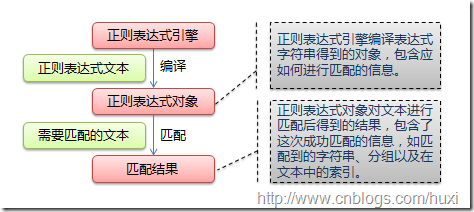
\includegraphics{images/pyreflow.png}
\caption{正则表达式}
\end{figure}

\hypertarget{ux6b63ux5219ux8868ux8fbeux5f0fux7684ux6784ux6210ux8981ux7d20}{%
\section{正则表达式的构成要素}\label{ux6b63ux5219ux8868ux8fbeux5f0fux7684ux6784ux6210ux8981ux7d20}}

正则表达式由四部分组成:定界符、原子、元字符、模式修饰符。

在python中,定界符可以不用写,使用raw字符串来表示正则表达式,更加方便。例如\texttt{r\textquotesingle{}\textbackslash{}d?i\textquotesingle{}}就表示是一个正则表达式,包含了元字符和模式修饰符。

\hypertarget{ux5b9aux754cux7b26}{%
\subsection{定界符}\label{ux5b9aux754cux7b26}}

定界符可以是任意非字母数字、非反斜线、非空白字符,常用``\texttt{/}''。

放在定界符中的最小的一个匹配单位,在一个正则表达式中,至少要有一个原子。正则表达式是一个从左到右匹配目标字符串的模式。

正则表达式的威力源于它可以在模式中拥有选择和重复的能力。一些字符被赋予特殊的涵义,使其不再单纯的代表自己,模式中的这种有特殊涵义的编码字符称为元字符。元字符用来修饰原子。

模式修饰符用来修正正则表达式进行,放在最右边。

\hypertarget{ux539fux5b50}{%
\subsection{原子}\label{ux539fux5b50}}

正则表达式中的原子可以是打印字符(键盘上的各种字母, 有的需要转义)、非打
印字符(如回车、制表符等)、转义符、子表达式(方括弧、圆括弧)。我们在理解正则表达式的时候,应该按照原子的顺序来解读。其他的子表达式(虽然是多个字符构成,但在逻辑上是一个原子),将在后续的内容进行详细讲解。

\hypertarget{ux5143ux5b57ux7b26}{%
\section{元字符}\label{ux5143ux5b57ux7b26}}

模式中有特殊涵义的编码字符称为元字符。元字符被赋予特殊的涵义,使其不再单纯的代表自己。如:

\begin{quote}
\texttt{\textbackslash{}d}表示数字,并不表示字母\texttt{d}。
\end{quote}

\hypertarget{ux5339ux914dux5355ux4e2aux5b57ux7b26ux7684ux5143ux5b57ux7b26}{%
\subsection{匹配单个字符的元字符}\label{ux5339ux914dux5355ux4e2aux5b57ux7b26ux7684ux5143ux5b57ux7b26}}

可以使用元字符匹配指定的单个字符,这是正则表达式的基础,正则表达式的其它功能都建立在对单个字符的匹配之上。

\begin{longtable}[]{@{}lll@{}}
\toprule
符号 & 元字符 & 匹配对象\tabularnewline
\midrule
\endhead
\texttt{.} & 点号 & 匹配单个任意字符(除换行)\tabularnewline
\texttt{{[}\ldots{}\ldots{}{]}} & 字符组 & 匹配单个列出的字符,可以使用连字符``\texttt{-}''表示范围\tabularnewline
\texttt{{[}\textbackslash{}\^{}\ldots{}\ldots{}{]}} & 排除型字符组 & 匹配单个未列出的字符\tabularnewline
\texttt{\textbackslash{}char} & 转义字符 & 如char是元字符,匹配char对应的普通字符\tabularnewline
\bottomrule
\end{longtable}

字符组(排除型字符组)是子表达式的一种,用方括弧来表示。方括弧\texttt{{[}{]}}内的多个字符会被认为是可选的一个字符。例如\texttt{{[}123456{]}}匹配1到6中的任意一个数字。\texttt{{[}123456{]}}还可以写成\texttt{{[}1-6{]}}。

\hypertarget{ux6b63ux5219ux8868ux8fbeux5f0fux4e2dux7684ux7279ux6b8aux5b57ux7b26}{%
\subsubsection{正则表达式中的特殊字符}\label{ux6b63ux5219ux8868ux8fbeux5f0fux4e2dux7684ux7279ux6b8aux5b57ux7b26}}

正则表达式特殊字符有:

\begin{Shaded}
\begin{Highlighting}[]
\NormalTok{. }\OperatorTok{\textbackslash{}} \OperatorTok{+} \OperatorTok{*}\NormalTok{ ? [ }\OperatorTok{^}\NormalTok{ ] $ ( ) \{ \} }\OperatorTok{=} \OperatorTok{!} \OperatorTok{<} \OperatorTok{>} \OperatorTok{|}\NormalTok{ : }\OperatorTok{-}
\end{Highlighting}
\end{Shaded}

当这些字符及定界符需要在模式中进行匹配时,需要在其前面加上反斜线进行转义。

\hypertarget{ux5e38ux7528ux8f6cux4e49ux7b26}{%
\subsection{常用转义符}\label{ux5e38ux7528ux8f6cux4e49ux7b26}}

常用转义符见下表:

\begin{longtable}[]{@{}ll@{}}
\toprule
符号 & 含义\tabularnewline
\midrule
\endhead
\texttt{\textbackslash{}t} & 制表符\tabularnewline
\texttt{\textbackslash{}n} & 换行符\tabularnewline
\texttt{\textbackslash{}r} & 回车符\tabularnewline
\texttt{\textbackslash{}s} & 任何``空白''字符(例如空格符、制表符、进纸符、回车换行符等)\tabularnewline
\texttt{\textbackslash{}S} & 除\texttt{\textbackslash{}s}之外的任何字符\tabularnewline
\texttt{\textbackslash{}w} & \texttt{{[}a-zA-Z0-9{]}}\tabularnewline
\texttt{\textbackslash{}W} & 除\texttt{\textbackslash{}w}之外的任何字符\tabularnewline
\texttt{\textbackslash{}d} & 数字\tabularnewline
\texttt{\textbackslash{}D} & 除\texttt{\textbackslash{}d}外的任何字符\tabularnewline
\bottomrule
\end{longtable}

如果要在正则表达式中使用反斜线,需要四个连用\texttt{\textbackslash{}\textbackslash{}\textbackslash{}\textbackslash{}}
,这里为什么是四个反斜线,原因在于:我们知道在正则概念上转义反斜线的写法为:\texttt{\textbackslash{}\textbackslash{}} 这个在正则表式下是能匹配出\texttt{\textbackslash{}},这是正则表达式引擎拿到的模式,但你也注意到了匹配出的\texttt{\textbackslash{}} 会转义后面的分隔符,所以我还需要一个反斜线来转义这个\texttt{\textbackslash{}} 。这样四个反斜线可理解为:前两个``生成''的\texttt{\textbackslash{}} 转义后两个``生成''的反斜杠。

\hypertarget{ux63d0ux4f9bux8ba1ux6570ux529fux80fdux7684ux5143ux5b57ux7b26}{%
\subsection{提供计数功能的元字符}\label{ux63d0ux4f9bux8ba1ux6570ux529fux80fdux7684ux5143ux5b57ux7b26}}

元字符还可以用来表示前置字符的数量,尤其是我们不知道字符内容的时候,这个功能就非常有用和高效。

\begin{longtable}[]{@{}lll@{}}
\toprule
符号 & 元字符 & 匹配对象\tabularnewline
\midrule
\endhead
\texttt{?} & 问号 & 匹配前置字符0-1次\tabularnewline
\texttt{*} & 星号 & 匹配前置字符0-N次\tabularnewline
\texttt{+} & 加号 & 匹配前置字符1-N次\tabularnewline
\texttt{\{n,m\}} & 区间量词 & 匹配前置字符n-m次\tabularnewline
\bottomrule
\end{longtable}

默认情况下,量词都是``贪婪''的,也就是说, 它们会在不导致模式匹配失败的前提下,尽可能多的匹配字符(直到最大允许的匹配次数)。然而,如果一个量词紧跟着一个 \texttt{?}(问号) 标记,它就会成为懒惰(非贪婪)模式, 它不再尽可能多的匹配,而是尽可能少的匹配。

\hypertarget{ux5339ux914dux4f4dux7f6eux7684ux5143ux5b57ux7b26}{%
\subsection{匹配位置的元字符}\label{ux5339ux914dux4f4dux7f6eux7684ux5143ux5b57ux7b26}}

元字符还可以用来表示位置,如一行的开始,单词的边界,或者是指定的某个位置。这种表示位置的元字符,又叫断言。一个断言就是一个对当前匹配位置之前或之后的字符的测试, 它不会实际消耗任何字符。

\begin{longtable}[]{@{}lll@{}}
\toprule
符号 & 元字符 & 匹配对象\tabularnewline
\midrule
\endhead
\texttt{\^{}} & 脱字符 & 匹配一行的开头位置\tabularnewline
\texttt{\$} & 美元符 & 匹配一行的结束位置\tabularnewline
\texttt{\textbackslash{}b} & 单词分界符 & 单词的分界位置\tabularnewline
\texttt{\textbackslash{}B} & 单词分界符 & 除单词分界位置的任何位置\tabularnewline
\texttt{(?\textless{}=...)} & 环视 & 匹配指定的位置\tabularnewline
\bottomrule
\end{longtable}

注意在子表达式内部,脱字符\texttt{\^{}}并不表示开头,而是表示``非''。

复杂的断言以子组的方式编码。 它有两种类型: 前瞻断言(匹配到的字符组的前面)和后瞻断言(匹配到的字符组的后面),每个类型中又分为肯定形式和否定形式。

\hypertarget{ux524dux77bbux65adux8a00}{%
\subsubsection{前瞻断言}\label{ux524dux77bbux65adux8a00}}

前瞻断言的肯定形式为\texttt{(?=\ldots{}\ldots{})}。

\begin{Shaded}
\begin{Highlighting}[]
\KeywordTok{$pattern}\NormalTok{ = }\StringTok{'/(?=中华人民共和国)/'}\OtherTok{;}
\CommentTok{// (?=中华人民共和国)匹配中华人民共和国的开始位置}
\KeywordTok{$string}\NormalTok{  = }\StringTok{'中华人民共和国,中华人民共和国,中华民国'}\OtherTok{;}
\KeywordTok{echo} \FunctionTok{preg_replace}\OtherTok{(}\KeywordTok{$pattern}\OtherTok{,} \StringTok{'我爱'}\OtherTok{,} \KeywordTok{$string}\OtherTok{),} \StringTok{"<br />"}\OtherTok{;}
\end{Highlighting}
\end{Shaded}

运行结果为:

\begin{Shaded}
\begin{Highlighting}[]
\NormalTok{我爱中华人民共和国,我爱中华人民共和国,中华民国}
\end{Highlighting}
\end{Shaded}

前瞻断言的否定形式为\texttt{(?!\ldots{}\ldots{})}:

\begin{Shaded}
\begin{Highlighting}[]
\KeywordTok{$pattern}\NormalTok{ = }\StringTok{'/(?!中华人民共和国)中华/'}\OtherTok{;}
\CommentTok{// // (?!中华人民共和国)匹配不是中华人民共和国的开始位置}
\KeywordTok{$string}\NormalTok{  = }\StringTok{'中华人民共和国,中华人民共和国,中华民国'}\OtherTok{;}
\KeywordTok{echo} \FunctionTok{preg_replace}\OtherTok{(}\KeywordTok{$pattern}\OtherTok{,} \StringTok{'我爱中华'}\OtherTok{,} \KeywordTok{$string}\OtherTok{),} \StringTok{"<br />"}\OtherTok{;}
\end{Highlighting}
\end{Shaded}

运行结果为:

\begin{Shaded}
\begin{Highlighting}[]
\NormalTok{中华人民共和国,中华人民共和国,我爱中华民国}
\end{Highlighting}
\end{Shaded}

\hypertarget{ux540eux77bbux65adux8a00}{%
\subsubsection{后瞻断言}\label{ux540eux77bbux65adux8a00}}

后瞻断言的肯定形式为\texttt{(?\textless{}=\ldots{}\ldots{})}:

\begin{Shaded}
\begin{Highlighting}[]
\KeywordTok{$pattern}\NormalTok{ = }\StringTok{'/(?<=中华人民共和国)/'}\OtherTok{;}
\CommentTok{// (?<=中华人民共和国)匹配中华人民共和国的结束位置}
\KeywordTok{$string}\NormalTok{  = }\StringTok{'中华人民共和国,中华人民共和国,中华民国'}\OtherTok{;}
\KeywordTok{echo} \FunctionTok{preg_replace}\OtherTok{(}\KeywordTok{$pattern}\OtherTok{,} \StringTok{'威武'}\OtherTok{,} \KeywordTok{$string}\OtherTok{),} \StringTok{"<br />"}\OtherTok{;}
\end{Highlighting}
\end{Shaded}

运行结果为:

\begin{Shaded}
\begin{Highlighting}[]
\NormalTok{中华人民共和国威武,中华人民共和国威武,中华民国}
\end{Highlighting}
\end{Shaded}

后瞻断言的否定形式为:\texttt{(?\textless{}!\ldots{}\ldots{})}

\begin{Shaded}
\begin{Highlighting}[]
\KeywordTok{$pattern}\NormalTok{ = }\StringTok{'/国(?<!中华人民共和国)/'}\OtherTok{;}
\CommentTok{// // (?<!中华人民共和国)匹配不是中华人民共和国的结束位置}
\KeywordTok{$string}\NormalTok{  = }\StringTok{'中华人民共和国,中华人民共和国,中华民国,美国'}\OtherTok{;}
\KeywordTok{echo} \FunctionTok{preg_replace}\OtherTok{(}\KeywordTok{$pattern}\OtherTok{,} \StringTok{'国人民'}\OtherTok{,} \KeywordTok{$string}\OtherTok{),} \StringTok{"<br />"}\OtherTok{;}
\end{Highlighting}
\end{Shaded}

运行结果为:

\begin{Shaded}
\begin{Highlighting}[]
\NormalTok{中华人民共和国,中华人民共和国,中华民国人民,美国人民}
\end{Highlighting}
\end{Shaded}

\hypertarget{ux65adux8a00ux7684ux7ec4ux5408}{%
\subsubsection{断言的组合}\label{ux65adux8a00ux7684ux7ec4ux5408}}

多个断言可以同时出现。断言子表达式的顺序无前后区分,只要同时满足断言条件的位置,都符合正则表达式模式要求。比如:

\begin{Shaded}
\begin{Highlighting}[]
\OtherTok{(?}\NormalTok{<=\textbackslash{}d\{}\DecValTok{3}\NormalTok{\}}\OtherTok{)(?}\NormalTok{<!}\DecValTok{999}\OtherTok{)}\NormalTok{foo}
\end{Highlighting}
\end{Shaded}

匹配前面有三个数字但不是 ``999'' 的字符串 ``foo''。

\hypertarget{ux5176ux4ed6ux5143ux5b57ux7b26}{%
\subsection{其他元字符}\label{ux5176ux4ed6ux5143ux5b57ux7b26}}

还有一些元字符用来分割表达式、设定引用方式等。

\begin{longtable}[]{@{}lll@{}}
\toprule
符号 & 元字符 & 匹配对象\tabularnewline
\midrule
\endhead
\textbar{} & 选择符 & 匹配任意分割的表达式\tabularnewline
\texttt{(\ldots{}\ldots{})} & 括号 & 限定多选结构的范围,标注量词的作用范围,为反向引用捕获文本\tabularnewline
\texttt{/1,/2,\ldots{}\ldots{}} & 反向引用 & 匹配之前的括号内的子表达式匹配的文本\tabularnewline
\bottomrule
\end{longtable}

竖线字符用于分离模式中的可选路径。 比如模式\texttt{com\textbar{}cn}匹配 ``com''或者``cn''。 竖线可以在模式中出现任意多个,并且允许有空的可选路径(匹配空字符串)。 匹配的处理从左到右尝试每一个可选路径,并且使用第一个成功匹配的。

括号中匹配的内容,可以保存到变量中,命名的规则为\texttt{(?\textless{}name\textgreater{})}:

\begin{Shaded}
\begin{Highlighting}[]
\KeywordTok{$pattern}\NormalTok{ = }\StringTok{'/<b>(?<title>.*?)<\textbackslash{}/b>/s'}\OtherTok{;}
\end{Highlighting}
\end{Shaded}

\hypertarget{ux6a21ux5f0fux4feeux9970ux7b26}{%
\section{模式修饰符}\label{ux6a21ux5f0fux4feeux9970ux7b26}}

模式修饰符是对整个正则表达式功能的调整。常用的模式修饰符如下:

\begin{enumerate}
\def\labelenumi{\arabic{enumi}.}
\tightlist
\item
  i 表示匹配大小写,在re模块中,可以使用\texttt{re.I}表示;
\item
  m 表示匹配多行,在re模块中,可以使用\texttt{re.M}表示;
\item
  s 可以点号元字符匹配所有字符, 包含换行,在re模块中,可以使用\texttt{re.S}表示。
\end{enumerate}

\hypertarget{ux5728pythonux4e2dux4f7fux7528ux6b63ux5219ux8868ux8fbeux5f0f}{%
\section{在Python中使用正则表达式}\label{ux5728pythonux4e2dux4f7fux7528ux6b63ux5219ux8868ux8fbeux5f0f}}

Python的re库全面实现了正则表达式的功能,下面将就常用功能进行示例。

\hypertarget{search}{%
\subsection{search()}\label{search}}

\texttt{search()}方法会扫描整个字符串,然后返回第一个成功匹配的结果,如果没有,则返回None。

\hypertarget{compile}{%
\subsection{compile()}\label{compile}}

\texttt{compile()}方法可以将正则字符串编译成正则表达式对象,以达到复用的目的,也还可以传入模式修饰符。

\hypertarget{findall}{%
\subsection{findall()}\label{findall}}

findall()方法会搜索整个字符串,然后返回所有匹配结果,如果没有,则返回None。

\begin{Shaded}
\begin{Highlighting}[]
\ImportTok{import}\NormalTok{ re}

\NormalTok{content }\OperatorTok{=} \StringTok{'dfdsfDDDDZ 23234'}
\NormalTok{pattern }\OperatorTok{=}\NormalTok{ re.}\BuiltInTok{compile}\NormalTok{(}\StringTok{'[a-z]'}\NormalTok{, re.I)}
\NormalTok{result }\OperatorTok{=}\NormalTok{ re.search(pattern, content)}
\BuiltInTok{print}\NormalTok{(result)}
\BuiltInTok{print}\NormalTok{(result.group())}
\BuiltInTok{print}\NormalTok{(result.span())}
\NormalTok{result }\OperatorTok{=}\NormalTok{ re.findall(pattern, content)}
\BuiltInTok{print}\NormalTok{(result)}
\end{Highlighting}
\end{Shaded}

上面的代码运行结果如下:

\begin{Shaded}
\begin{Highlighting}[]
\OperatorTok{<}\ExtensionTok{re.Match}\NormalTok{ object}\KeywordTok{;} \VariableTok{span=(}\NormalTok{0, 1}\VariableTok{)}\NormalTok{, }\VariableTok{match=}\StringTok{'d'}\OperatorTok{>}
\ExtensionTok{d}
\KeywordTok{(}\ExtensionTok{0}\NormalTok{, 1}\KeywordTok{)}
\NormalTok{[}\StringTok{'d'}\NormalTok{, }\StringTok{'f'}\NormalTok{, }\StringTok{'d'}\NormalTok{, }\StringTok{'s'}\NormalTok{, }\StringTok{'f'}\NormalTok{, }\StringTok{'D'}\NormalTok{, }\StringTok{'D'}\NormalTok{, }\StringTok{'D'}\NormalTok{, }\StringTok{'D'}\NormalTok{, }\StringTok{'Z'}\NormalTok{]}
\end{Highlighting}
\end{Shaded}

可以看出,\texttt{search()}方法和\texttt{findall()}方法存在的区别。

\hypertarget{argparse}{%
\chapter{命令行参数模块argparse}\label{argparse}}

Argparse模块主要用来开发类似于shell中原生命令那样用户友好的命令行工具。使用该模块可以定义必需参数、可选参数,还能自动生成帮助和使用说明。

先看一个简单例子:

\begin{Shaded}
\begin{Highlighting}[]
\CommentTok{#! /Users/ncsxbmu/anaconda3/bin/python}
\CommentTok{# coding=utf-8}

\ImportTok{import}\NormalTok{ sys}
\BuiltInTok{print}\NormalTok{ (}\StringTok{"文件名 = "}\NormalTok{, sys.argv[}\DecValTok{0}\NormalTok{])}
\ControlFlowTok{for}\NormalTok{ i }\KeywordTok{in} \BuiltInTok{range}\NormalTok{(}\DecValTok{1}\NormalTok{, }\BuiltInTok{len}\NormalTok{(sys.argv)):}
    \BuiltInTok{print}\NormalTok{ (}\StringTok{"参数}\SpecialCharTok{%s}\StringTok{ = }\SpecialCharTok\NormalTok{(i, sys.argv[i]))}
\end{Highlighting}
\end{Shaded}

假设上述代码存放在名为\texttt{test.py}的文件中,则上述代码输出结果如下:

\begin{Shaded}
\begin{Highlighting}[]
 \CommentTok{# 不带参数调用}
\NormalTok{👉  }\ExtensionTok{python}\NormalTok{ test.py}
\FunctionTok{file}\NormalTok{ =  test.py}

\CommentTok{# 带多个参数调用}
\NormalTok{👉  }\ExtensionTok{python}\NormalTok{ test.py 1 3}
\FunctionTok{file}\NormalTok{ =  test.py}
\NormalTok{参数}\ExtensionTok{1}\NormalTok{ = 1}
\NormalTok{参数}\ExtensionTok{2}\NormalTok{ = 3}
\end{Highlighting}
\end{Shaded}

从这个例子中我们可以看出,利用内置模块sys.argv能非常方便地获取参数内容。但这个模块在处理复杂参数时不够简洁和方便。因此,我们需要更加强大的argparse模块,该模块的用法是:

\begin{enumerate}
\def\labelenumi{\arabic{enumi}.}
\tightlist
\item
  创建解析器
\item
  添加参数
\item
  解析参数
\end{enumerate}

下面分别讲解:

\hypertarget{ux521bux5efaux89e3ux6790ux5668}{%
\section{创建解析器}\label{ux521bux5efaux89e3ux6790ux5668}}

使用\texttt{ArgumentParser}类创建参数解析器,参数都为关键字参数。语法为:

\begin{Shaded}
\begin{Highlighting}[]
\KeywordTok{class}\NormalTok{ argparse.ArgumentParser(prog}\OperatorTok{=}\VariableTok{None}\NormalTok{, usage}\OperatorTok{=}\VariableTok{None}\NormalTok{, description}\OperatorTok{=}\VariableTok{None}\NormalTok{, epilog}\OperatorTok{=}\VariableTok{None}\NormalTok{, parents}\OperatorTok{=}\NormalTok{[], formatter_class}\OperatorTok{=}\NormalTok{argparse.HelpFormatter, prefix_chars}\OperatorTok{=}\StringTok{'-'}\NormalTok{, fromfile_prefix_chars}\OperatorTok{=}\VariableTok{None}\NormalTok{, argument_default}\OperatorTok{=}\VariableTok{None}\NormalTok{, conflict_handler}\OperatorTok{=}\StringTok{'error'}\NormalTok{, add_help}\OperatorTok{=}\VariableTok{True}\NormalTok{, allow_abbrev}\OperatorTok{=}\VariableTok{True}\NormalTok{)}
\end{Highlighting}
\end{Shaded}

其中主要参数说明如下:

\begin{enumerate}
\def\labelenumi{\arabic{enumi}.}
\tightlist
\item
  prog - 程序名称,默认值为程序文件名。
\item
  usage - 程序用法描述,默认根据添加的参数生成。
\item
  description - 参数说明信息之前的文本默认为空。
\item
  epilog - 参数说明信息之后的文本,默认为空。
\item
  parents - 需要包含的父解析器。
\item
  add\_help - 添加 -h/--help 选项,默认为真。
\item
  allow\_abbrev - 是否允许参数缩写,默认为真。
\end{enumerate}

例如:

\begin{Shaded}
\begin{Highlighting}[]
\CommentTok{#! /Users/ncsxbmu/anaconda3/bin/python}
\CommentTok{# coding=utf-8}

\ImportTok{import}\NormalTok{ argparse}

\NormalTok{parser }\OperatorTok{=}\NormalTok{ argparse.ArgumentParser()}
\NormalTok{parser }\OperatorTok{=}\NormalTok{ argparse.ArgumentParser(description }\OperatorTok{=} \StringTok{'合并多个markdown文件并转化为docx文件'}\NormalTok{)}
\NormalTok{parser.print_help()}
\end{Highlighting}
\end{Shaded}

运行结果如下:

\begin{Shaded}
\begin{Highlighting}[]
\NormalTok{ 👉  }\ExtensionTok{python}\NormalTok{ test.py}

\ExtensionTok{usage}\NormalTok{: test.py [-h]}

\NormalTok{合并多个}\ExtensionTok{markdown}\NormalTok{文件并转化为docx文件}

\ExtensionTok{optional}\NormalTok{ arguments:}
  \ExtensionTok{-h}\NormalTok{, --help  show this help message and exit}
\end{Highlighting}
\end{Shaded}

\hypertarget{ux6dfbux52a0ux53c2ux6570ux9009ux9879}{%
\section{添加参数选项}\label{ux6dfbux52a0ux53c2ux6570ux9009ux9879}}

使用\texttt{add\_argument}类来添加参数,以及如何解析参数,语法如下:

\begin{Shaded}
\begin{Highlighting}[]
\NormalTok{ArgumentParser.add_argument(name }\KeywordTok{or}\NormalTok{ flags...[, action][, nargs][, const][, default][, }\BuiltInTok{type}\NormalTok{][, choices][, required][, }\BuiltInTok{help}\NormalTok{][, metavar][, dest])}
\end{Highlighting}
\end{Shaded}

\hypertarget{name-or-flags}{%
\subsection{name or flags}\label{name-or-flags}}

name 或者 flags 用来指定参数名称,或者参数列表,其中以\texttt{-}开始的参数为可选参数。例如:

\begin{Shaded}
\begin{Highlighting}[]
\ImportTok{import}\NormalTok{ argparse}

\NormalTok{parser }\OperatorTok{=}\NormalTok{ argparse.ArgumentParser()}
\NormalTok{parser }\OperatorTok{=}\NormalTok{ argparse.ArgumentParser(description }\OperatorTok{=} \StringTok{'合并多个markdown文件并转化为docx文件'}\NormalTok{)}
\NormalTok{parser.add_argument(}\StringTok{'echo'}\NormalTok{)}
\NormalTok{parser.add_argument(}\StringTok{'-s'}\NormalTok{,}\StringTok{'--source'}\NormalTok{)}

\NormalTok{args }\OperatorTok{=}\NormalTok{ parser.parse_args()}

\BuiltInTok{print}\NormalTok{ (args.echo)}
\BuiltInTok{print}\NormalTok{ (args.source)}
\end{Highlighting}
\end{Shaded}

上述代码增加了1个必需参数\texttt{echo},和1个可选参数\texttt{source},测试结果如下:

\begin{Shaded}
\begin{Highlighting}[]
\NormalTok{👉  }\ExtensionTok{test.py}\NormalTok{ hello -s sun}
\ExtensionTok{hello}
\ExtensionTok{sun}

\NormalTok{👉  }\ExtensionTok{test.py}\NormalTok{ hello --source sun}
\ExtensionTok{hello}
\ExtensionTok{sun}

\NormalTok{ 👉  }\ExtensionTok{test.py}\NormalTok{ --source sun}
\ExtensionTok{usage}\NormalTok{: test.py [-h] [-s SOURCE] echo}
\ExtensionTok{test.py}\NormalTok{: error: the following arguments are required: echo}

\NormalTok{ 👉  }\ExtensionTok{test.py}\NormalTok{ hello}
\ExtensionTok{hello}
\ExtensionTok{None}
\end{Highlighting}
\end{Shaded}

结果显示,如果缺少必填参数,则会报错,而可选参数即可用短参数形式,也可用长参数形式。

\hypertarget{help}{%
\subsection{help}\label{help}}

不论是必选参数还是可选参数,强烈建议使用help参数添加说明文字,该说明文字会自动生成在help结果中。

\begin{Shaded}
\begin{Highlighting}[]
\ImportTok{import}\NormalTok{ argparse}

\NormalTok{parser }\OperatorTok{=}\NormalTok{ argparse.ArgumentParser()}
\NormalTok{parser }\OperatorTok{=}\NormalTok{ argparse.ArgumentParser(description }\OperatorTok{=} \StringTok{'合并多个markdown文件并转化为docx文件'}\NormalTok{)}
\NormalTok{parser.add_argument(}\StringTok{'source'}\NormalTok{,}\BuiltInTok{help}\OperatorTok{=}\StringTok{'待转换的文件'}\NormalTok{)}
\NormalTok{parser.add_argument(}\StringTok{'-st'}\NormalTok{,}\StringTok{'--sourcetype'}\NormalTok{,}\BuiltInTok{help}\OperatorTok{=}\StringTok{'转换前的格式'}\NormalTok{)}

\NormalTok{args }\OperatorTok{=}\NormalTok{ parser.parse_args()}

\BuiltInTok{print}\NormalTok{ (args.source)}
\BuiltInTok{print}\NormalTok{ (args.sourcetype)}
\end{Highlighting}
\end{Shaded}

当使用-h或者--help输出帮助信息时,结果如下:

\begin{Shaded}
\begin{Highlighting}[]
\NormalTok{ 👉  }\ExtensionTok{test.py}\NormalTok{ -h}
\ExtensionTok{usage}\NormalTok{: test.py [-h] [-st SOURCETYPE] source}

\NormalTok{合并多个}\ExtensionTok{markdown}\NormalTok{文件并转化为docx文件}

\ExtensionTok{positional}\NormalTok{ arguments:}
  \BuiltInTok{source}\NormalTok{                待转换的文件}

\ExtensionTok{optional}\NormalTok{ arguments:}
  \ExtensionTok{-h}\NormalTok{, --help            show this help message and exit}
  \ExtensionTok{-st}\NormalTok{ SOURCETYPE, --sourcetype SOURCETYPE}
\NormalTok{                        转换前的格式}
\end{Highlighting}
\end{Shaded}

可见,argparse模块已经非常贴心地按照help参数值,生成了帮助信息。

\hypertarget{defaultux548ctype}{%
\subsection{default和type}\label{defaultux548ctype}}

default参数用来指定参数默认值,type用来指定参数类型(默认值是string),这两个参数经常一起使用,用来限定参数值。

\begin{Shaded}
\begin{Highlighting}[]
\ImportTok{import}\NormalTok{ argparse}

\NormalTok{parser }\OperatorTok{=}\NormalTok{ argparse.ArgumentParser()}
\NormalTok{parser }\OperatorTok{=}\NormalTok{ argparse.ArgumentParser(description }\OperatorTok{=} \StringTok{'合并多个markdown文件并转化为docx文件'}\NormalTok{)}
\NormalTok{parser.add_argument(}\StringTok{'--source'}\NormalTok{,}\StringTok{'-s'}\NormalTok{,}\BuiltInTok{help}\OperatorTok{=}\StringTok{'待转换的文件'}\NormalTok{,default}\OperatorTok{=}\StringTok{'source.md'}\NormalTok{)}
\NormalTok{parser.add_argument(}\StringTok{'-st'}\NormalTok{,}\StringTok{'--sourcetype'}\NormalTok{,}\BuiltInTok{help}\OperatorTok{=}\StringTok{'转换前的格式'}\NormalTok{)}
\NormalTok{parser.add_argument(}\StringTok{'-l'}\NormalTok{,}\StringTok{'--level'}\NormalTok{,}\BuiltInTok{help}\OperatorTok{=}\StringTok{'压缩级别'}\NormalTok{,}\BuiltInTok{type}\OperatorTok{=}\BuiltInTok{int}\NormalTok{,default}\OperatorTok{=}\DecValTok{1}\NormalTok{)}

\NormalTok{args }\OperatorTok{=}\NormalTok{ parser.parse_args()}

\BuiltInTok{print}\NormalTok{ (args.source)}
\BuiltInTok{print}\NormalTok{ (args.sourcetype)}
\BuiltInTok{print}\NormalTok{ (args.level)}
\end{Highlighting}
\end{Shaded}

在上述代码中,增加了三个可选参数,并设定了默认值和类型,结果输出如下:

\begin{Shaded}
\begin{Highlighting}[]
\NormalTok{ 👉  }\ExtensionTok{test.py}
\ExtensionTok{source.md}
\ExtensionTok{None}
\ExtensionTok{1}

\NormalTok{ 👉  }\ExtensionTok{test.py}\NormalTok{ -l 3}
\ExtensionTok{source.md}
\ExtensionTok{None}
\ExtensionTok{3}
\end{Highlighting}
\end{Shaded}

可以看到,指定的默认值都起了作用。

\hypertarget{ux53c2ux6570ux89e3ux6790}{%
\section{参数解析}\label{ux53c2ux6570ux89e3ux6790}}

只有使用\texttt{parse\_args()}方法对添加的参数进行解析后,才能在命令行中使用参数,用法很简单,已在前面的代码中多次出现。

\hypertarget{ux5c0fux7ed3}{%
\section{小结}\label{ux5c0fux7ed3}}

agrparse模块的功能还有很多,这里只是介绍了入门的用法,还有很多细节没有提到,详细信息请查看官方文档。

\hypertarget{ux53c2ux8003ux6587ux732e}{%
\section{参考文献}\label{ux53c2ux8003ux6587ux732e}}

\begin{enumerate}
\def\labelenumi{\arabic{enumi}.}
\tightlist
\item
  \href{https://docs.python.org/3/library/argparse.html}{argparse模块官方手册}
\item
  \href{https://www.jianshu.com/p/fef2d215b91d}{argparse用法总结}
\end{enumerate}

\hypertarget{part-ux6570ux636eux6293ux53d6}{%
\part{数据抓取}\label{part-ux6570ux636eux6293ux53d6}}

\hypertarget{spider}{%
\chapter{网络爬虫}\label{spider}}

网络爬虫就是能够按照一定规则,自动收集网络中的数据的程序。

\hypertarget{ux7f51ux7edcux722cux866bux539fux7406}{%
\section{网络爬虫原理}\label{ux7f51ux7edcux722cux866bux539fux7406}}

\begin{enumerate}
\def\labelenumi{\arabic{enumi}.}
\tightlist
\item
  请求网页,获取网页源代码
\item
  提取信息
\item
  存储数据
\item
  自动化程序
\end{enumerate}

网页本质上是一个存储在指定位置的文本文件(不一定是静态的,可能是由远程计算机根据一定条件计算出来的),因此,网络爬虫的任务,就是获取远程文本文件,然后,对文件进行分析,提取出我们想要的数据。

\hypertarget{httpux8bf7ux6c42ux539fux7406}{%
\section{HTTP请求原理}\label{httpux8bf7ux6c42ux539fux7406}}

HTTP遵循请求(Request)/应答(Response)模型。

Web浏览器向Web服务器发送请求,Web服务器处理请求并返回适当的应答。所有HTTP连接都被构造成一套请求和应答。

\begin{figure}
\centering
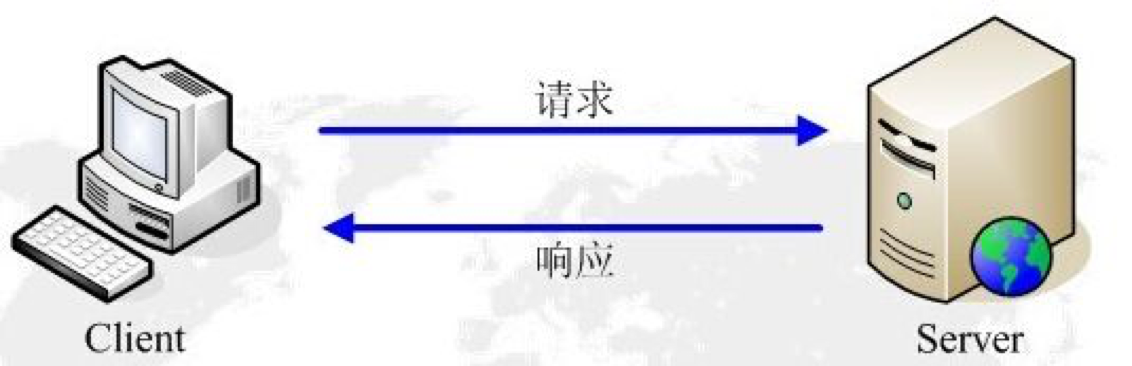
\includegraphics{images/http.png}
\caption{PNG}
\end{figure}

浏览器作为一个客户端,向服务器端发送了一次浏览该地址所对应的网页的请求

服务器同意了客户端的请求

客户端把服务器端的文件下载到本地

浏览器对文件进行解释、展现

\hypertarget{url}{%
\subsection{URL}\label{url}}

统一资源定位符(Uniform Resource Locator) 是互联网上标准资源的地址。互联网上的每个文件都有一个唯一的URL。
基本URL包含模式(或称协议)、服务器名称(或IP地址)、路径和文件名,

如:协议://授权/路径?查询

\begin{verbatim}
http://alumni.xjtu.edu.cn:9090/donation/namelist?pageNo=1&pageSize=10&billnum=&donateUserName=&orderWay=&donationid=0
\end{verbatim}

爬虫最主要的处理对象就是URL,它根据URL地址取得所需要的文件内容,然后对它进行进一步的处理。

\hypertarget{ux8bf7ux6c42ux65b9ux5f0f}{%
\subsection{请求方式}\label{ux8bf7ux6c42ux65b9ux5f0f}}

\hypertarget{get}{%
\subsubsection{GET}\label{get}}

GET方法是默认的HTTP请求方法,我们日常用GET方法来提交表单数据,然而用GET方法提交的表单数据只经过了简单的编码,同时它将作为URL的一部分向Web服务器发送。

\hypertarget{post}{%
\subsubsection{POST}\label{post}}

POST方法是GET方法的一个替代方法,它主要是向Web服务器提交表单数据,尤其是大批量的数据。POST方法克服了GET方法的一些缺点。通过POST方法提交表单数据时,数据不是作为URL请求的一部分而是作为标准数据传送给Web服务器,这就克服了GET方法中的信息无法保密和数据量太小的缺点。

\hypertarget{requestsux5305}{%
\subsection{requests包}\label{requestsux5305}}

Requests 是 Python 中的 HTTP 库,Requests库允许你发送符合标准的 HTTP/1.1 请求,无需手工劳动。你不需要手动为 URL 添加查询字串,也不需要对 POST 数据进行表单编码。Keep-alive 和 HTTP 连接池的功能是 100\% 自动化的。

官方网站:\url{http://cn.python-requests.org/zh_CN/latest/}

安装方式:

\begin{verbatim}
pip install requests
\end{verbatim}

\hypertarget{ux7f16ux7801}{%
\section{编码}\label{ux7f16ux7801}}

\hypertarget{ux7f16ux7801ux65b9ux5f0f}{%
\subsection{编码方式}\label{ux7f16ux7801ux65b9ux5f0f}}

\begin{enumerate}
\def\labelenumi{\arabic{enumi}.}
\tightlist
\item
  ASCII编码:是对英语字符和二进制之间的关系做的统一规定
\item
  GBK编码:是汉字编码标准之一,是在 GB2312-80 标准基础上的内码扩展规范,使用了双字节编码
\item
  GB2312编码:适用于汉字处理、汉字通信等系统之间的信息交换
\item
  GB18030编码:国家标准GB18030-2005《信息技术 中文编码字符集》是我国继GB2312-1980和GB13000.1-1993之后最重要的汉字编码标准,是我国计算机系统必须遵循的基础性标准之一。 GB18030有两个版本:GB18030-2000和GB18030-2005。GB18030-2000是GBK的取代版本,它的主要特点是在GBK基础上增加了CJK统一汉字扩充A的汉字。GB18030-2005的主要特点是在GB18030-2000基础上增加了CJK统一汉字扩充B的汉字。
\item
  UTF-8编码:是 Unicode Transformation Format - 8 bit 的缩写。它是可变长的编码方式,可以使用1\textasciitilde4个字节表示一个字符,可根据不同的符号而变化字节长度
\item
  Unicode编码:这是一种世界上所有字符的编码。当然了它没有规定的存储方式
\end{enumerate}

\hypertarget{ux7f16ux7801ux8f6cux6362}{%
\subsection{编码转换}\label{ux7f16ux7801ux8f6cux6362}}

通常是要以Unicode作为中间编码进行转换,即先将其他编码的字符串解码(decode)成 Unicode,再从 Unicode编码(encode)成另一种编码。

\hypertarget{ux5b58ux50a8}{%
\section{存储}\label{ux5b58ux50a8}}

存储的时候,可以将字符串编码之后,再存储到文件。

\hypertarget{ux5b58ux50a8ux5230ux6587ux4ef6}{%
\subsection{存储到文件}\label{ux5b58ux50a8ux5230ux6587ux4ef6}}

使用open函数,可以创建文件,并将内容写入到文件中。

\begin{Shaded}
\begin{Highlighting}[]
\NormalTok{f }\OperatorTok{=} \BuiltInTok{open}\NormalTok{(}\StringTok{'xjtu.html'}\NormalTok{, }\StringTok{'w'}\NormalTok{)}
\NormalTok{f.write(content.encode(}\StringTok{'utf-8'}\NormalTok{))}
\NormalTok{f.close()}
\end{Highlighting}
\end{Shaded}

\hypertarget{httplib}{%
\chapter{HTTP库}\label{httplib}}

Python提供了功能齐全的HTTP库,使用这些库,我们只需要关心请求的地址是什么,参数是什么,不用关心更底层的技术,大大降低了信息抓取的难度。最基础的HTTP库有urllib、request等等。

\hypertarget{urllib}{%
\section{urllib}\label{urllib}}

Urllib是Python3内置的http库,它包含四个模块:

\begin{enumerate}
\def\labelenumi{\arabic{enumi}.}
\tightlist
\item
  request
\item
  error
\item
  parse
\item
  robotparser
\end{enumerate}

\hypertarget{ux53d1ux9001ux8bf7ux6c42}{%
\subsection{发送请求}\label{ux53d1ux9001ux8bf7ux6c42}}

使用urllib的request模块,可以方便地实现请求的发送,并得到响应。

\begin{Shaded}
\begin{Highlighting}[]
\ImportTok{import}\NormalTok{ urllib.request}

\NormalTok{rqs }\OperatorTok{=}\NormalTok{ urllib.request.urlopen(}\StringTok{'http://www.baidu.com'}\NormalTok{)}
\NormalTok{html }\OperatorTok{=}\NormalTok{ rqs.read()}
\BuiltInTok{print}\NormalTok{(html)}
\end{Highlighting}
\end{Shaded}

\texttt{request()}方法返回\texttt{HTTPResponse}类型的对象,具有一些处理信息的属性和方法。其中最基本的是\texttt{urlopen()}方法,可以完成最基本的请求。它的使用方法如下:

\begin{Shaded}
\begin{Highlighting}[]
\NormalTok{urllib.request.urlopen(url, data}\OperatorTok{=}\VariableTok{None}\NormalTok{, [timeout, ]}\OperatorTok{*}\NormalTok{, cafile}\OperatorTok{=}\VariableTok{None}\NormalTok{, capath}\OperatorTok{=}\VariableTok{None}\NormalTok{, cadefault}\OperatorTok{=}\VariableTok{False}\NormalTok{, context}\OperatorTok{=}\VariableTok{None}\NormalTok{)}
\end{Highlighting}
\end{Shaded}

\hypertarget{dataux53c2ux6570}{%
\subsubsection{data参数}\label{dataux53c2ux6570}}

如果要添加\texttt{data}参数,则需要使用\texttt{byte()}方法构造一个字节流编码格式的内容。使用\texttt{data}参数后,请求方式就变成了\texttt{POST}方式。

\begin{Shaded}
\begin{Highlighting}[]
\ImportTok{import}\NormalTok{ urllib.request}
\ImportTok{import}\NormalTok{ urllib.parse}

\NormalTok{data }\OperatorTok{=} \BuiltInTok{bytes}\NormalTok{(urllib.parse.urlencode(\{}\StringTok{'word'}\NormalTok{:}\StringTok{'hello'}\NormalTok{\}),encoding}\OperatorTok{=}\StringTok{'utf8'}\NormalTok{)}
\NormalTok{rqs }\OperatorTok{=}\NormalTok{ urllib.request.urlopen(}\StringTok{'http://httpbin.org/post'}\NormalTok{,data }\OperatorTok{=}\NormalTok{ data)}

\BuiltInTok{print}\NormalTok{(rqs.read())}
\end{Highlighting}
\end{Shaded}

\hypertarget{timeoutux53c2ux6570}{%
\subsubsection{timeout参数}\label{timeoutux53c2ux6570}}

timeout参数用于设置超时时间,单位为秒,默认为全局默认时间。

\begin{Shaded}
\begin{Highlighting}[]
\ImportTok{import}\NormalTok{ urllib.request}
\ImportTok{import}\NormalTok{ urllib.parse}
\ImportTok{import}\NormalTok{ socket}
\ImportTok{import}\NormalTok{ urllib.error}

\NormalTok{data }\OperatorTok{=} \BuiltInTok{bytes}\NormalTok{(urllib.parse.urlencode(\{}\StringTok{'word'}\NormalTok{:}\StringTok{'hello'}\NormalTok{\}),encoding}\OperatorTok{=}\StringTok{'utf8'}\NormalTok{)}

\ControlFlowTok{try}\NormalTok{:}
\NormalTok{    rqs }\OperatorTok{=}\NormalTok{ urllib.request.urlopen(}\StringTok{'http://httpbin.org/post'}\NormalTok{,data }\OperatorTok{=}\NormalTok{ data,timeout}\OperatorTok{=}\FloatTok{0.1}\NormalTok{)}
\ControlFlowTok{except}\NormalTok{ urllib.error.URLError }\ImportTok{as}\NormalTok{ e:}
    \ControlFlowTok{if} \BuiltInTok{isinstance}\NormalTok{(e.reason,socket.timeout):}
        \BuiltInTok{print}\NormalTok{(}\StringTok{'time out'}\NormalTok{)}
\end{Highlighting}
\end{Shaded}

通过设置timeout参数来实现超时处理,是非常有用的策略。

\hypertarget{requestux65b9ux6cd5}{%
\subsubsection{Request方法}\label{requestux65b9ux6cd5}}

如果要在请求中加入头信息,就需要使用Request类。

\begin{Shaded}
\begin{Highlighting}[]
\ImportTok{import}\NormalTok{ urllib.request}
\ImportTok{import}\NormalTok{ urllib.parse}
\ImportTok{import}\NormalTok{ socket}
\ImportTok{import}\NormalTok{ urllib.error}

\NormalTok{url }\OperatorTok{=} \StringTok{'http://httpbin.org/post'}
\NormalTok{headers }\OperatorTok{=}\NormalTok{ \{}
    \StringTok{'User-Agent'}\NormalTok{:}\StringTok{'Mozilla/4.0 (compatible; MSIE 5.5; Windows NT)'}\NormalTok{,}
    \StringTok{'Host'}\NormalTok{:}\StringTok{'httpbin.org'}
\NormalTok{\}}
\BuiltInTok{dict} \OperatorTok{=}\NormalTok{ \{}
    \StringTok{'name'}\NormalTok{:}\StringTok{'Yang'}
\NormalTok{\}}

\NormalTok{data }\OperatorTok{=} \BuiltInTok{bytes}\NormalTok{(urllib.parse.urlencode(}\BuiltInTok{dict}\NormalTok{),encoding}\OperatorTok{=}\StringTok{'utf8'}\NormalTok{)}
\NormalTok{req }\OperatorTok{=}\NormalTok{ urllib.request.Request(url}\OperatorTok{=}\NormalTok{url,data }\OperatorTok{=}\NormalTok{ data,headers}\OperatorTok{=}\NormalTok{headers)}

\ControlFlowTok{try}\NormalTok{:}
\NormalTok{   response }\OperatorTok{=}\NormalTok{ urllib.request.urlopen(req,timeout}\OperatorTok{=}\DecValTok{3}\NormalTok{)}
\ControlFlowTok{except}\NormalTok{ urllib.error.URLError }\ImportTok{as}\NormalTok{ e:}
    \ControlFlowTok{if} \BuiltInTok{isinstance}\NormalTok{(e.reason,socket.timeout):}
        \BuiltInTok{print}\NormalTok{(}\StringTok{'time out'}\NormalTok{)}

\BuiltInTok{print}\NormalTok{(response.read())}
\end{Highlighting}
\end{Shaded}

依然用urlopen()方法来发送这个请求,只不过参数不是url,而是Request类型的对象。Request对象的参数如下:

\begin{Shaded}
\begin{Highlighting}[]
\KeywordTok{class}\NormalTok{ urllib.request.Request(url, data}\OperatorTok{=}\VariableTok{None}\NormalTok{, headers}\OperatorTok{=}\NormalTok{\{\}, origin_req_host}\OperatorTok{=}\VariableTok{None}\NormalTok{, unverifiable}\OperatorTok{=}\VariableTok{False}\NormalTok{, method}\OperatorTok{=}\VariableTok{None}\NormalTok{)}
\end{Highlighting}
\end{Shaded}

\begin{enumerate}
\def\labelenumi{\arabic{enumi}.}
\tightlist
\item
  url是必选参数
\item
  data必须是字节流类型。
\item
  headers是一个字典
\item
  origin\_req\_host是请求方的host名称或者ip地址
\item
  unverfiable表示请求是否无法验证(如读取图像的权限)
\item
  method的值为GET、POST、PUT等等。
\end{enumerate}

\hypertarget{ux5904ux7406ux5f02ux5e38}{%
\subsection{处理异常}\label{ux5904ux7406ux5f02ux5e38}}

urllib的error模块定义了由request模块阐释的异常。如果出现了问题,request模块便会抛出error模块定义的异常。

\hypertarget{urlerror}{%
\subsubsection{URLError}\label{urlerror}}

URLError类继承自OSError,由request模块产生的异常都可以通过这个类捕获。它具有一个属性reason,即返回错误的原因。例如,我们访问一个不存在的页面:

\begin{Shaded}
\begin{Highlighting}[]
\ImportTok{from}\NormalTok{ urllib }\ImportTok{import}\NormalTok{ request,error}

\ControlFlowTok{try}\NormalTok{:}
\NormalTok{    response }\OperatorTok{=}\NormalTok{ request.urlopen(}\StringTok{'http://yangzh.cn/php.html'}\NormalTok{)}
\ControlFlowTok{except}\NormalTok{ error.URLError }\ImportTok{as}\NormalTok{ e:}
    \BuiltInTok{print}\NormalTok{(e.reason)}
\end{Highlighting}
\end{Shaded}

运行结果为\texttt{Not\ Found}。程序没有直接报错,而是输出上述内容,这样我们就具备了处理意外的能力,使得程序更加健壮。

\hypertarget{httperror}{%
\subsubsection{HTTPError}\label{httperror}}

HTTPError是URLError的子类,所以可以先捕获HTTPError,然后再捕获URLError,如果正常,则用else来处理,这是一种更加稳妥的异常处理方式。例如:

\begin{Shaded}
\begin{Highlighting}[]
\ImportTok{from}\NormalTok{ urllib }\ImportTok{import}\NormalTok{ request,error}

\ControlFlowTok{try}\NormalTok{:}
\NormalTok{    response }\OperatorTok{=}\NormalTok{ request.urlopen(}\StringTok{'http://yangzh.cn/php.html'}\NormalTok{)}
\ControlFlowTok{except}\NormalTok{ error.HTTPError }\ImportTok{as}\NormalTok{ e:}
    \BuiltInTok{print}\NormalTok{(e.reason,e.code,e.headers,sep}\OperatorTok{=}\StringTok{'}\CharTok{\textbackslash{}n}\StringTok{'}\NormalTok{)}
\ControlFlowTok{except}\NormalTok{ error.URLError }\ImportTok{as}\NormalTok{ e:}
    \BuiltInTok{print}\NormalTok{(e.reason)}
\ControlFlowTok{else}\NormalTok{:}
    \BuiltInTok{print}\NormalTok{(}\StringTok{'请求成功'}\NormalTok{)}
\end{Highlighting}
\end{Shaded}

HTTPError有3个属性:

\begin{enumerate}
\def\labelenumi{\arabic{enumi}.}
\tightlist
\item
  code为HTTP状态码。
\item
  reason为错误原因,其值可能是字符串,也可能是对象。
\item
  headers为响应头信息。
\end{enumerate}

\hypertarget{ux89e3ux6790ux94feux63a5}{%
\subsection{解析链接}\label{ux89e3ux6790ux94feux63a5}}

urllib中的parse模块,可以实现URL的抽取、合并以及链接转换,在数据抓取中使用频率很高。

\hypertarget{urlparse}{%
\subsubsection{urlparse()}\label{urlparse}}

\texttt{urlparse()}可以实现URL的识别和分段,例如:

\begin{Shaded}
\begin{Highlighting}[]
\ImportTok{from}\NormalTok{ urllib.parse }\ImportTok{import}\NormalTok{ urlparse}

\NormalTok{url }\OperatorTok{=} \StringTok{'https://cn.bing.com/search.php?q=python#id-1'}
\NormalTok{result }\OperatorTok{=}\NormalTok{ urlparse(url)}
\BuiltInTok{print}\NormalTok{(}\BuiltInTok{type}\NormalTok{(result),result,sep}\OperatorTok{=}\StringTok{'}\CharTok{\textbackslash{}n}\StringTok{'}\NormalTok{)}
\end{Highlighting}
\end{Shaded}

运行结果如下:

\begin{Shaded}
\begin{Highlighting}[]
\OperatorTok{<}\KeywordTok{class} \StringTok{'urllib.parse.ParseResult'}\OperatorTok{>}
\NormalTok{ParseResult(scheme}\OperatorTok{=}\StringTok{'https'}\NormalTok{, netloc}\OperatorTok{=}\StringTok{'cn.bing.com'}\NormalTok{, path}\OperatorTok{=}\StringTok{'/search.php'}\NormalTok{, params}\OperatorTok{=}\StringTok{''}\NormalTok{, query}\OperatorTok{=}\StringTok{'q=python'}\NormalTok{, fragment}\OperatorTok{=}\StringTok{'id-1'}\NormalTok{)}
\end{Highlighting}
\end{Shaded}

从结果可以看出,该方法将URL分解为六个部分:

\begin{enumerate}
\def\labelenumi{\arabic{enumi}.}
\tightlist
\item
  scheme表示协议
\item
  netloc表示域名、主机
\item
  path表示主机中的路径
\item
  params表示参数
\item
  query表示查询条件,GET方式提交请求会产生此类信息
\item
  fragment表示地址片段,指向页面内部锚点
\end{enumerate}

\hypertarget{urlencode}{%
\subsubsection{urlencode()}\label{urlencode}}

urlencode()用于构造GET请求,如:

\begin{Shaded}
\begin{Highlighting}[]
\ImportTok{from}\NormalTok{ urllib.parse }\ImportTok{import}\NormalTok{ urlparse,urlencode}

\NormalTok{params }\OperatorTok{=}\NormalTok{\{}
    \StringTok{'name'}\NormalTok{:}\StringTok{'yangzh'}\NormalTok{,}
    \StringTok{'age'}\NormalTok{:}\StringTok{'21'}
\NormalTok{\}}

\NormalTok{base_url }\OperatorTok{=} \StringTok{'http://www.yangzh.cn?'}
\NormalTok{url }\OperatorTok{=}\NormalTok{ base_url }\OperatorTok{+}\NormalTok{ urlencode(params)}

\BuiltInTok{print}\NormalTok{(url)}
\end{Highlighting}
\end{Shaded}

结果输出为\texttt{http://www.yangzh.cn?name=yangzh\&age=21}。

\hypertarget{parse_qs}{%
\subsubsection{parse\_qs()}\label{parse_qs}}

该函数可以将GET请求参数转化为字典,例如:

\begin{Shaded}
\begin{Highlighting}[]
\ImportTok{from}\NormalTok{ urllib.parse }\ImportTok{import}\NormalTok{ urlparse,urlencode,parse_qs}

\NormalTok{params }\OperatorTok{=}\NormalTok{\{}
    \StringTok{'name'}\NormalTok{:}\StringTok{'yangzh'}\NormalTok{,}
    \StringTok{'age'}\NormalTok{:}\StringTok{'21'}
\NormalTok{\}}

\NormalTok{base_url }\OperatorTok{=} \StringTok{'http://www.yangzh.cn?'}
\NormalTok{url }\OperatorTok{=}\NormalTok{ base_url }\OperatorTok{+}\NormalTok{ urlencode(params)}

\NormalTok{result }\OperatorTok{=}\NormalTok{ urlparse(url)}

\BuiltInTok{print}\NormalTok{(url)}
\BuiltInTok{print}\NormalTok{(result.query,parse_qs(result.query),sep}\OperatorTok{=}\StringTok{'}\CharTok{\textbackslash{}n}\StringTok{'}\NormalTok{)}
\end{Highlighting}
\end{Shaded}

将打印出:

\begin{Shaded}
\begin{Highlighting}[]
\ExtensionTok{http}\NormalTok{://www.yangzh.cn?name=yangzh}\KeywordTok{&}\VariableTok{age=}\NormalTok{21}
\VariableTok{name=}\NormalTok{yangzh}\KeywordTok{&}\VariableTok{age=}\NormalTok{21}
\NormalTok{\{}\StringTok{'name'}\NormalTok{: [}\StringTok{'yangzh'}\NormalTok{], }\StringTok{'age'}\NormalTok{: [}\StringTok{'21'}\NormalTok{]\}}
\end{Highlighting}
\end{Shaded}

\hypertarget{urlux7f16ux7801}{%
\subsubsection{URL编码}\label{urlux7f16ux7801}}

\texttt{quote()}方法可以将特殊内容(如空格、中文等)转化为URL编码的格式,\texttt{unquote()}方法可以对URL编码进行解码。

\hypertarget{ux4f7fux7528requests}{%
\section{使用requests}\label{ux4f7fux7528requests}}

与urllib库相比,requests库要更为简洁和人性化,功能也更为丰富。

\hypertarget{ux5b89ux88c5requests}{%
\subsection{安装requests}\label{ux5b89ux88c5requests}}

使用pip工具,可以非常简单地实现requests库的安装:

\begin{Shaded}
\begin{Highlighting}[]
\ExtensionTok{pip}\NormalTok{ install requests}
\end{Highlighting}
\end{Shaded}

\hypertarget{ux53d1ux8d77ux8bf7ux6c42}{%
\subsection{发起请求}\label{ux53d1ux8d77ux8bf7ux6c42}}

利用params参数,可以非常方便地构造请求地址:

\begin{Shaded}
\begin{Highlighting}[]
\ImportTok{import}\NormalTok{ requests}
\NormalTok{data }\OperatorTok{=}\NormalTok{ \{}
    \StringTok{"name"}\NormalTok{: }\StringTok{"yangjh"}\NormalTok{,}
    \StringTok{"age"}\NormalTok{: }\DecValTok{20}
\NormalTok{\}}
\NormalTok{r }\OperatorTok{=}\NormalTok{ requests.get(}\StringTok{'http://httpbin.org/get'}\NormalTok{, params}\OperatorTok{=}\NormalTok{data)}
\BuiltInTok{print}\NormalTok{(r.text)}
\end{Highlighting}
\end{Shaded}

上述代码将会构造\texttt{http://httpbin.org/get?name=yangjh\&age=20}的地址,并以字符串的形式返回请求结果。对于返回结果是JSON格式,还可以使用json()方法转化为字典。

利用headers参数,可以构造出浏览器标识信息。例如:

\begin{Shaded}
\begin{Highlighting}[]
\NormalTok{headers }\OperatorTok{=}\NormalTok{ \{}
    \StringTok{'User-Agent'}\NormalTok{: }\StringTok{'Mozilla/5.0 (Macintosh; Intel Mac OS X 10.13; rv:63.0) Gecko/20100101 Firefox/63.0'}
\NormalTok{\}}
\NormalTok{r }\OperatorTok{=}\NormalTok{ requests.get(}\StringTok{'https://www.zhihu.com/explore'}\NormalTok{, headers}\OperatorTok{=}\NormalTok{headers)}
\end{Highlighting}
\end{Shaded}

除了GET方法之外,还可以使用POST、PUT、DELETE等方法。

\hypertarget{ux5904ux7406ux54cdux5e94}{%
\subsubsection{处理响应}\label{ux5904ux7406ux54cdux5e94}}

可以通过\texttt{text}、\texttt{content}、\texttt{status\_code}、\texttt{headers}、\texttt{cookies}、\texttt{url}、\texttt{history}等属性获得服务器返回请求的内容。其中\texttt{status\_code}的值和HTTP状态码一一对应,比如\texttt{404}可以用\texttt{requests.codes.not\_found}来对比。

\hypertarget{ux4f1aux8bddux7ef4ux6301}{%
\subsubsection{会话维持}\label{ux4f1aux8bddux7ef4ux6301}}

使用Session方法,可以维持同一个会话,不用每次都设置cookies的值,相当于在浏览器中新建选项卡打开网址,而不是重新打开一个浏览器。

\begin{Shaded}
\begin{Highlighting}[]
\NormalTok{s }\OperatorTok{=}\NormalTok{ requests.Session()}
\NormalTok{s.get(}\StringTok{'http://httpbin.org/cookies/set/age/20'}\NormalTok{)}
\NormalTok{r }\OperatorTok{=}\NormalTok{ s.get(}\StringTok{'http://httpbin.org/cookies'}\NormalTok{)}
\BuiltInTok{print}\NormalTok{(r.text)}
\end{Highlighting}
\end{Shaded}

使用Session,可以模拟登陆成功之后再进行下一步操作。

\hypertarget{ux8d85ux65f6ux8bbeux7f6e}{%
\subsubsection{超时设置}\label{ux8d85ux65f6ux8bbeux7f6e}}

为了防止长时间等待,提高效率,我们有必要通过timeout属性设置超时时间,例如:

\begin{Shaded}
\begin{Highlighting}[]
\NormalTok{r }\OperatorTok{=}\NormalTok{ requests.get(}\StringTok{'https://www.baidu.com'}\NormalTok{, timeout}\OperatorTok{=}\DecValTok{1}\NormalTok{)}
\BuiltInTok{print}\NormalTok{(r.status_code)}

\NormalTok{r }\OperatorTok{=}\NormalTok{ requests.get(}\StringTok{'https://www.taobao.com'}\NormalTok{, timeout}\OperatorTok{=}\NormalTok{(}\DecValTok{5}\NormalTok{, }\DecValTok{30}\NormalTok{))}
\BuiltInTok{print}\NormalTok{(r.status_code)}
\end{Highlighting}
\end{Shaded}

如果timeout只有1个值,则指的是从发出请求到服务器返回响应的总时间;如果timeout的值是有俩值的元组,则第一个元素为请求时间,第二个元素为响应时间。

\hypertarget{requestux5bf9ux8c61}{%
\subsubsection{Request对象}\label{requestux5bf9ux8c61}}

可以先构造好请求,再使用send方法发送请求,这样可以达到处理不同请求的目的。

\begin{Shaded}
\begin{Highlighting}[]
\NormalTok{url }\OperatorTok{=} \StringTok{'http://httpbin.org/post'}
\NormalTok{data }\OperatorTok{=}\NormalTok{ \{}
    \StringTok{'age'}\NormalTok{: }\DecValTok{20}
\NormalTok{\}}
\NormalTok{headers }\OperatorTok{=}\NormalTok{ \{}
    \StringTok{'User-Agent'}\NormalTok{: }\StringTok{'Mozilla/5.0 (Macintosh; Intel Mac OS X 10.13; rv:63.0) Gecko/20100101 Firefox/63.0'}
\NormalTok{\}}
\NormalTok{s }\OperatorTok{=}\NormalTok{ requests.Session()}
\NormalTok{req }\OperatorTok{=}\NormalTok{ requests.Request(}\StringTok{'POST'}\NormalTok{, url, data}\OperatorTok{=}\NormalTok{data, headers}\OperatorTok{=}\NormalTok{headers)}
\NormalTok{preped }\OperatorTok{=}\NormalTok{ s.prepare_request(req)}
\NormalTok{r }\OperatorTok{=}\NormalTok{ s.send(preped)}
\BuiltInTok{print}\NormalTok{(r.text)}
\end{Highlighting}
\end{Shaded}

使用Request这个对象,我们可以方便地构造出请求。

\hypertarget{ux7f51ux9875ux7f16ux7801ux68c0ux6d4bux53caux8f6cux6362}{%
\section{网页编码检测及转换}\label{ux7f51ux9875ux7f16ux7801ux68c0ux6d4bux53caux8f6cux6362}}

有时,页面虽然申明的编码方式是\texttt{utf-8},但输出的时候却产生乱码,因此需要先检测页面编码方式,再将其转化为utf编码。例如:

\begin{Shaded}
\begin{Highlighting}[]
\NormalTok{html }\OperatorTok{=}\NormalTok{ requests.get(url, headers}\OperatorTok{=}\NormalTok{headers, cookies}\OperatorTok{=}\NormalTok{jar)}
\BuiltInTok{print}\NormalTok{(html.text.encode(html.encoding).decode(}\StringTok{'utf8'}\NormalTok{))}
\end{Highlighting}
\end{Shaded}

使用requests库中的\texttt{encoding}属性,可以获得返回对象的编码方式,然后按照其编码方式编码,再按照utf8方式解码,即可得到UTF编码方式的内容。

\hypertarget{ux53c2ux8003ux8d44ux6599-2}{%
\section{参考资料}\label{ux53c2ux8003ux8d44ux6599-2}}

\begin{enumerate}
\def\labelenumi{\arabic{enumi}.}
\tightlist
\item
  \url{https://docs.python.org/3/library/urllib.html}
\item
  \url{http://cn.python-requests.org/zh_CN/latest/}
\end{enumerate}

\hypertarget{pyquery}{%
\chapter{Pyquery}\label{pyquery}}

Pyquery是一个使用jQuery方式进行高效解析的库。与使用正则表达式相比,借助于诸如pyquery之类的解析库,开发人员可以写出可读性更强的网页解析代码。

\hypertarget{ux5b89ux88c5}{%
\section{安装}\label{ux5b89ux88c5}}

\begin{Shaded}
\begin{Highlighting}[]
\ExtensionTok{pip3}\NormalTok{ install pyquery}
\end{Highlighting}
\end{Shaded}

\hypertarget{ux521dux59cbux5316}{%
\section{初始化}\label{ux521dux59cbux5316}}

所谓初始化,就是引入pyquery库,获取解析文本。例如:

\begin{Shaded}
\begin{Highlighting}[]
\ImportTok{from}\NormalTok{ pyquery }\ImportTok{import}\NormalTok{ PyQuery }\ImportTok{as}\NormalTok{ pq}
\ImportTok{import}\NormalTok{ requests}

\NormalTok{html }\OperatorTok{=}\NormalTok{ requests.get(}\StringTok{'http://www.yangzh.cn'}\NormalTok{).text}
\NormalTok{doc }\OperatorTok{=}\NormalTok{ pq(html)}
\BuiltInTok{print}\NormalTok{(doc(}\StringTok{'title'}\NormalTok{).text())}
\end{Highlighting}
\end{Shaded}

上面的代码使用requests库获得网页内容,再使用pyquery库进行解析,获取网页标题元素的内容。

\hypertarget{ux83b7ux53d6ux4fe1ux606f}{%
\section{获取信息}\label{ux83b7ux53d6ux4fe1ux606f}}

使用pyquery获取网页信息的方式和jQuery是一致的,先通过选择符进行对象的选择,再对选择的对象进行操作。

\hypertarget{ux901aux8fc7ux9009ux62e9ux7b26ux9009ux5b9aux5143ux7d20}{%
\subsection{通过选择符选定元素}\label{ux901aux8fc7ux9009ux62e9ux7b26ux9009ux5b9aux5143ux7d20}}

\begin{Shaded}
\begin{Highlighting}[]
\NormalTok{titles }\OperatorTok{=}\NormalTok{ doc(}\StringTok{'ul.kanban-List li h3'}\NormalTok{).items()}
\NormalTok{times }\OperatorTok{=}\NormalTok{ doc(}\StringTok{'ul.kanban-List li p span.redTxt'}\NormalTok{).items()}
\NormalTok{locations }\OperatorTok{=}\NormalTok{ doc(}\StringTok{'ul.kanban-List li b.localIcon'}\NormalTok{).parent().items()}
\end{Highlighting}
\end{Shaded}

\hypertarget{ux901aux8fc7ux8fedux4ee3ux83b7ux53d6ux6700ux7ec8ux7ed3ux679c}{%
\subsection{通过迭代获取最终结果}\label{ux901aux8fc7ux8fedux4ee3ux83b7ux53d6ux6700ux7ec8ux7ed3ux679c}}

使用\texttt{text()}方法,可以获取元素的内容,当然,还可以使用\texttt{attr()}获取指定属性的值。利用zip函数,可以对多个迭代器进行遍历:

\begin{Shaded}
\begin{Highlighting}[]
\KeywordTok{def}\NormalTok{ merge_info():}
    \ControlFlowTok{for}\NormalTok{ title, time, location }\KeywordTok{in} \BuiltInTok{zip}\NormalTok{(titles, times, locations):}
        \CommentTok{# print(title.text(), time.text(), location.text())}
        \ControlFlowTok{if} \StringTok{'江安'} \KeywordTok{in}\NormalTok{ location.text():}
            \ControlFlowTok{yield}\NormalTok{ \{}
                \StringTok{'title'}\NormalTok{: title.text(),}
                \StringTok{'time'}\NormalTok{: time.text(),}
                \StringTok{'location'}\NormalTok{: location.text()}
\NormalTok{            \}}
\end{Highlighting}
\end{Shaded}

\hypertarget{ux53c2ux8003ux8d44ux6599-3}{%
\section{参考资料}\label{ux53c2ux8003ux8d44ux6599-3}}

\begin{enumerate}
\def\labelenumi{\arabic{enumi}.}
\tightlist
\item
  \url{https://pyquery.readthedocs.io/en/latest/}
\item
  \url{https://jquery.com/}
\end{enumerate}

\hypertarget{databases}{%
\chapter{数据存储}\label{databases}}

获取到的信息,我们通常使用文件、数据库的形式存储起来,以便再次利用。

使用文件的方式保存数据,用法比较简单,而数据库的方式则分为使用关系型数据库和非关系型数据库,其各自的代表数据库产品是MySQL和MongoDB,皆为开源产品,从性能和安全性角度都具有很强的竞争力。因而,下面介绍这两个数据库在Python中的使用。

\hypertarget{mysqlux7684ux5b58ux50a8}{%
\section{MySQL的存储}\label{mysqlux7684ux5b58ux50a8}}

成功从页面获取信息后,我们可以将其保存到文件中,也可以存储到数据库中。显然,使用数据库拥有更多后续分析的便利,我们采用常见的关系型数据库MySQL作为信息的保存方式。

\hypertarget{ux5b89ux88c5pymysqlux548cmysql}{%
\subsection{安装PyMySQL和MySQL}\label{ux5b89ux88c5pymysqlux548cmysql}}

使用Homebrew和pip工具分别安装MySQL和PyMySQL。

\hypertarget{ux8fdeux63a5ux6570ux636eux5e93}{%
\subsection{连接数据库}\label{ux8fdeux63a5ux6570ux636eux5e93}}

对数据库的使用和其它语言是一致的,无非就是连接数据库,发送指令,接收结果。

\begin{Shaded}
\begin{Highlighting}[]
\ImportTok{import}\NormalTok{ pymysql}
\NormalTok{db }\OperatorTok{=}\NormalTok{ pymysql.}\ExtensionTok{connect}\NormalTok{(host}\OperatorTok{=}\StringTok{'localhost'}\NormalTok{, user}\OperatorTok{=}\StringTok{'user'}\NormalTok{,password}\OperatorTok{=}\StringTok{'password'}\NormalTok{, port}\OperatorTok{=}\DecValTok{3306}\NormalTok{)}
\end{Highlighting}
\end{Shaded}

使用pymysql的\texttt{connect()}方法,设置必要的信息,可以连接到MySQL数据库。

还可以直接连接到MySQL中已经存在的库:

\begin{Shaded}
\begin{Highlighting}[]
\NormalTok{connection }\OperatorTok{=}\NormalTok{ pymysql.}\ExtensionTok{connect}\NormalTok{(host}\OperatorTok{=}\StringTok{'localhost'}\NormalTok{,}
\NormalTok{                             user}\OperatorTok{=}\StringTok{'user'}\NormalTok{,}
\NormalTok{                             password}\OperatorTok{=}\StringTok{'passwd'}\NormalTok{,}
\NormalTok{                             db}\OperatorTok{=}\StringTok{'db'}\NormalTok{,}
\NormalTok{                             charset}\OperatorTok{=}\StringTok{'utf8mb4'}\NormalTok{)}
\end{Highlighting}
\end{Shaded}

\hypertarget{ux5bf9ux6570ux636eux5e93ux8fdbux884cux64cdux4f5c}{%
\subsection{对数据库进行操作}\label{ux5bf9ux6570ux636eux5e93ux8fdbux884cux64cdux4f5c}}

连接到数据库后,可以使用游标cursor()方法对数据库进行各种操作。

\hypertarget{ux521bux5efaux6570ux636eux5e93}{%
\subsubsection{创建数据库}\label{ux521bux5efaux6570ux636eux5e93}}

使用SQL语句,就可以创建数据库,创建数据库的语句如下:

\begin{Shaded}
\begin{Highlighting}[]
\ImportTok{import}\NormalTok{ pymysql}

\NormalTok{db }\OperatorTok{=}\NormalTok{ pymysql.}\ExtensionTok{connect}\NormalTok{(host}\OperatorTok{=}\StringTok{'localhost'}\NormalTok{, user}\OperatorTok{=}\StringTok{'root'}\NormalTok{,}
\NormalTok{                     password}\OperatorTok{=}\StringTok{'mysql'}\NormalTok{, port}\OperatorTok{=}\DecValTok{3306}\NormalTok{)}

\NormalTok{cursor }\OperatorTok{=}\NormalTok{ db.cursor()}
\NormalTok{sql }\OperatorTok{=} \StringTok{"CREATE DATABASE spiders DEFAULT CHARACTER SET utf8"}
\NormalTok{cursor.execute(sql)}
\NormalTok{db.commit()}
\NormalTok{db.close()}
\end{Highlighting}
\end{Shaded}

使用游标方法\texttt{cursor()}创建游标对象,用\texttt{execute()}方法执行SQL语句,再使用\texttt{commit()}提交,最后使用\texttt{close()}方法关闭数据库连接。

\hypertarget{ux521bux5efaux6570ux636eux8868}{%
\subsubsection{创建数据表}\label{ux521bux5efaux6570ux636eux8868}}

使用SQL语句可以创建数据表,当然前提是连接到数据库。

\begin{Shaded}
\begin{Highlighting}[]
\CommentTok{# coding=utf-8}
\ImportTok{import}\NormalTok{ pymysql}

\NormalTok{db }\OperatorTok{=}\NormalTok{ pymysql.}\ExtensionTok{connect}\NormalTok{(host}\OperatorTok{=}\StringTok{'localhost'}\NormalTok{, user}\OperatorTok{=}\StringTok{'root'}\NormalTok{,}
\NormalTok{                     password}\OperatorTok{=}\StringTok{'mysql'}\NormalTok{, db}\OperatorTok{=}\StringTok{'spiders'}\NormalTok{)}

\NormalTok{cursor }\OperatorTok{=}\NormalTok{ db.cursor()}
\NormalTok{sql }\OperatorTok{=} \StringTok{"CREATE TABLE IF NOT EXISTS students (id VARCHAR(255) NOT NULL, name VARCHAR(255) NOT NULL, age INT NOT NULL, PRIMARY KEY (id))"}
\NormalTok{cursor.execute(sql)}
\NormalTok{db.commit()}

\NormalTok{db.close()}
\end{Highlighting}
\end{Shaded}

SQL语句的语法,可以参照MySQL参考手册,也可借助于类似phpMyadmin之类的工具进行生成和检测。

\hypertarget{ux63d2ux5165ux66f4ux65b0ux5220ux9664ux6570ux636e}{%
\subsubsection{插入、更新、删除数据}\label{ux63d2ux5165ux66f4ux65b0ux5220ux9664ux6570ux636e}}

使用INSERT语句,可以插入数据到数据表:

\begin{Shaded}
\begin{Highlighting}[]
\CommentTok{# coding=utf-8}
\ImportTok{import}\NormalTok{ pymysql}

\NormalTok{db }\OperatorTok{=}\NormalTok{ pymysql.}\ExtensionTok{connect}\NormalTok{(host}\OperatorTok{=}\StringTok{'localhost'}\NormalTok{, user}\OperatorTok{=}\StringTok{'root'}\NormalTok{,}
\NormalTok{                     password}\OperatorTok{=}\StringTok{'mysql'}\NormalTok{, db}\OperatorTok{=}\StringTok{'spiders'}\NormalTok{)}

\NormalTok{cursor }\OperatorTok{=}\NormalTok{ db.cursor()}

\BuiltInTok{id} \OperatorTok{=} \StringTok{'2018'}
\NormalTok{user }\OperatorTok{=} \StringTok{'yangjh'}
\NormalTok{age }\OperatorTok{=} \DecValTok{18}

\NormalTok{sql }\OperatorTok{=} \StringTok{'INSERT INTO students(id,name,age) values(}\SpecialCharTok{%s}\StringTok{,}\SpecialCharTok{%s}\StringTok{,}\SpecialCharTok{%s}\StringTok{)'}
\ControlFlowTok{try}\NormalTok{:}
\NormalTok{    cursor.execute(sql, (}\BuiltInTok{id}\NormalTok{, user, age))}
\NormalTok{    db.commit()}
\ControlFlowTok{except}\NormalTok{:}
\NormalTok{    db.rollback()}
\NormalTok{db.close()}
\end{Highlighting}
\end{Shaded}

插入、更新和删除操作都是对数据库进行更改的操作,这些操作的写法是:

\begin{Shaded}
\begin{Highlighting}[]
\ControlFlowTok{try}\NormalTok{:}
\NormalTok{    cursor.execute(sql)}
\NormalTok{    db.commit()}
\ControlFlowTok{except}\NormalTok{:}
\NormalTok{    db.rollback()}
\end{Highlighting}
\end{Shaded}

使用rollback()方法可以回滚执行失败的操作,保持事务的原子性(atomicity),使用异常处理,可以方便地实现业务回滚。

\hypertarget{ux67e5ux8be2ux6570ux636e}{%
\subsubsection{查询数据}\label{ux67e5ux8be2ux6570ux636e}}

使用\texttt{while}循环加\texttt{fetchone()}方法循环获取数据:

\begin{Shaded}
\begin{Highlighting}[]
\NormalTok{sql }\OperatorTok{=} \StringTok{'SELECT * FROM students WHERE age <=20'}
\ControlFlowTok{try}\NormalTok{:}
\NormalTok{    cursor.execute(sql)}
\NormalTok{    row }\OperatorTok{=}\NormalTok{ cursor.fetchone()}
    \ControlFlowTok{while}\NormalTok{ row:}
        \BuiltInTok{print}\NormalTok{(row, row[}\DecValTok{0}\NormalTok{])}
\NormalTok{        row }\OperatorTok{=}\NormalTok{ cursor.fetchone()}
\ControlFlowTok{except}\NormalTok{:}
    \BuiltInTok{print}\NormalTok{(}\StringTok{'出错啦!'}\NormalTok{)}
\NormalTok{db.close()}
\end{Highlighting}
\end{Shaded}

\hypertarget{mongodb}{%
\section{MongoDB}\label{mongodb}}

MongoDB 是一款开源的非关系数据库管理软件,性能优异,在诸多大型项目中表现良好,是非关系型数据库的首选。

\hypertarget{ux5728macosux4e2dux7684ux5b89ux88c5}{%
\subsection{在macOS中的安装}\label{ux5728macosux4e2dux7684ux5b89ux88c5}}

MongoDB 只支持macOS 10.11及以后的产品。

\hypertarget{ux4f7fux7528ux5305ux7ba1ux7406ux5de5ux5177ux5b89ux88c5}{%
\subsubsection{使用包管理工具安装}\label{ux4f7fux7528ux5305ux7ba1ux7406ux5de5ux5177ux5b89ux88c5}}

我们使用在macOS 中的包管理工具Homebrew进行安装。

\begin{Shaded}
\begin{Highlighting}[]
\ExtensionTok{brew}\NormalTok{ install mongodb}
\end{Highlighting}
\end{Shaded}

上述指令将安装MongoDB的最新发行版,并会自动安装MongoDB所需要的依赖环境。

\hypertarget{ux8fd0ux884cux524dux7684ux51c6ux5907}{%
\subsubsection{运行前的准备}\label{ux8fd0ux884cux524dux7684ux51c6ux5907}}

在启动MongoDB之前,需要创建MongoDB读写数据的目录,默认情况下,MongoDB会以\texttt{/data/db}为默认目录。下面的命令将创建默认的\texttt{/data/db}目录:

\begin{Shaded}
\begin{Highlighting}[]
\FunctionTok{mkdir}\NormalTok{ -p /data/db}
\end{Highlighting}
\end{Shaded}

创建目录后,为给目录指定读写权限。然后使用如下命令将MongoDB加入到系统服务中,以便每次启动时都可自动启动MongoDB服务。

\begin{Shaded}
\begin{Highlighting}[]
\ExtensionTok{brew}\NormalTok{ services start mongodb}
\end{Highlighting}
\end{Shaded}

\hypertarget{ux5b89ux88c5pymongoux5e93}{%
\subsubsection{安装PyMongo库}\label{ux5b89ux88c5pymongoux5e93}}

启动虚拟python环境,然后通过pip安装PyMongo库:

\begin{Shaded}
\begin{Highlighting}[]
\NormalTok{ 👉  }\BuiltInTok{source}\NormalTok{ bin/activate}
\KeywordTok{(}\ExtensionTok{spider}\KeywordTok{)} 
\NormalTok{ 👉  }\ExtensionTok{pip3}\NormalTok{ install pymongo}
\ExtensionTok{Collecting}\NormalTok{ pymongo}
  \ExtensionTok{Downloading}\NormalTok{ https://files.pythonhosted.org/packages/d7/ac/d2e324c1f9bcf653fa106785371a16b4709506a35b04948655de8b961a85/pymongo-3.7.2-cp37-cp37m-macosx_10_9_x86_64.whl (307kB)}
    \ExtensionTok{100%} \KeywordTok{|}\NormalTok{████████████████████████████████}\KeywordTok{|} \ExtensionTok{317kB}\NormalTok{ 1.6MB/s }
\ExtensionTok{Installing}\NormalTok{ collected packages: pymongo}
\ExtensionTok{Successfully}\NormalTok{ installed pymongo-3.7.2}
\end{Highlighting}
\end{Shaded}

\hypertarget{ux5b89ux88c5robo-3t}{%
\subsubsection{安装Robo 3T}\label{ux5b89ux88c5robo-3t}}

MongoDB并没有默认的图形化管理工具,只提供Mongo shell的命令行方式。为了方便,我们还可以使用诸如Robo 3T这样的图形化管理工具进行查询、修改等管理工作。使用Homebrew安装:

\begin{Shaded}
\begin{Highlighting}[]
\ExtensionTok{brew}\NormalTok{ install robo-3t}
\end{Highlighting}
\end{Shaded}

安装后,在应用程序中找到robo-3t,进行必要的配置(指定主机名和端口),即可对MongoDB进行管理。

\hypertarget{ux8fdeux63a5mongodb}{%
\subsection{连接MongoDB}\label{ux8fdeux63a5mongodb}}

使用PyMongo库,可以在Python中对MongoDB进行操作,连接到数据库,使用MongoClient方法即可:

\begin{Shaded}
\begin{Highlighting}[]
\ImportTok{import}\NormalTok{ pymongo}

\NormalTok{client }\OperatorTok{=}\NormalTok{ pymongo.MongoClient(}\StringTok{'mongodb://localhost:27017'}\NormalTok{)}
\end{Highlighting}
\end{Shaded}

\hypertarget{ux6307ux5b9aux6570ux636eux5e93}{%
\subsection{指定数据库}\label{ux6307ux5b9aux6570ux636eux5e93}}

MongoDB中建立和使用数据库非常简单,直接指定数据库名称即可,如果该数据库不存在,MongoDB就会创建该数据库:

\begin{Shaded}
\begin{Highlighting}[]
\NormalTok{db }\OperatorTok{=}\NormalTok{ client[}\StringTok{'weibo'}\NormalTok{]}
\end{Highlighting}
\end{Shaded}

\hypertarget{ux6307ux5b9aux96c6ux5408}{%
\subsection{指定集合}\label{ux6307ux5b9aux96c6ux5408}}

MongoDB中的集合(collection),相当于MySQL等关系型数据库中的数据表(table),具体的信息,必须指定一个集合,才能进行存入、修改等操作。使用Collection对象,即可指定集合:

\begin{Shaded}
\begin{Highlighting}[]
\ImportTok{import}\NormalTok{ pymongo}
\NormalTok{client }\OperatorTok{=}\NormalTok{ pymongo.MongoClient(}\StringTok{'mongodb://localhost:27017'}\NormalTok{)}
\NormalTok{db }\OperatorTok{=}\NormalTok{ client[}\StringTok{'weibo'}\NormalTok{]}
\NormalTok{collection }\OperatorTok{=}\NormalTok{ db[}\StringTok{'yangjh'}\NormalTok{]}
\end{Highlighting}
\end{Shaded}

\hypertarget{ux63d2ux5165ux6570ux636e}{%
\subsection{插入数据}\label{ux63d2ux5165ux6570ux636e}}

推荐使用\texttt{insert\_one()}和\texttt{insert\_many()}方法来分别插入单条记录和多条记录。

\begin{Shaded}
\begin{Highlighting}[]
\NormalTok{card }\OperatorTok{=}\NormalTok{ \{}
    \StringTok{"id"}\NormalTok{: }\StringTok{"20183210"}\NormalTok{,}
    \StringTok{"name"}\NormalTok{: }\StringTok{'yangjh'}\NormalTok{,}
    \StringTok{"age"}\NormalTok{: }\DecValTok{20}\NormalTok{,}
    \StringTok{'gender'}\NormalTok{: }\StringTok{'male'}
\NormalTok{\}}

\NormalTok{result }\OperatorTok{=}\NormalTok{ collection.insert_one(card)}
\BuiltInTok{print}\NormalTok{(result)}
\BuiltInTok{print}\NormalTok{(result.inserted_id)}
\end{Highlighting}
\end{Shaded}

运行结果为:

\begin{Shaded}
\begin{Highlighting}[]
\OperatorTok{<}\ExtensionTok{pymongo.results.InsertOneResult}\NormalTok{ object at 0x10436da48}\OperatorTok{>}
\ExtensionTok{5bf8b3f897c32c4128ae8f6f}
\end{Highlighting}
\end{Shaded}

\texttt{insert\_one()}方法返回一个对象,调用其\texttt{inserted\_id}属性,可以获得\texttt{\_id}字段的值。

还可以使用\texttt{insert\_many()}方法,一次插入多条记录:

\begin{Shaded}
\begin{Highlighting}[]
\NormalTok{card1 }\OperatorTok{=}\NormalTok{ \{}
    \StringTok{"id"}\NormalTok{: }\StringTok{"20183211"}\NormalTok{,}
    \StringTok{"name"}\NormalTok{: }\StringTok{'yangzh'}\NormalTok{,}
    \StringTok{"age"}\NormalTok{: }\DecValTok{20}\NormalTok{,}
    \StringTok{'gender'}\NormalTok{: }\StringTok{'male'}
\NormalTok{\}}

\NormalTok{card2 }\OperatorTok{=}\NormalTok{ \{}
    \StringTok{"id"}\NormalTok{: }\StringTok{"20183212"}\NormalTok{,}
    \StringTok{"name"}\NormalTok{: }\StringTok{'yangzhh'}\NormalTok{,}
    \StringTok{"age"}\NormalTok{: }\DecValTok{40}\NormalTok{,}
    \StringTok{'gender'}\NormalTok{: }\StringTok{'female'}
\NormalTok{\}}
\NormalTok{result }\OperatorTok{=}\NormalTok{ collection.insert_many([card1, card2])}
\BuiltInTok{print}\NormalTok{(result)}
\BuiltInTok{print}\NormalTok{(result.inserted_ids)}
\end{Highlighting}
\end{Shaded}

\hypertarget{ux67e5ux8be2ux6570ux636e-1}{%
\subsection{查询数据}\label{ux67e5ux8be2ux6570ux636e-1}}

查询数据,使用\texttt{find\_one()}或\texttt{find()}方法进行查询,顾名思义,\texttt{find\_one()}方法查询结果是单条,而\texttt{find()}方法返回全部结果。

\begin{Shaded}
\begin{Highlighting}[]
\NormalTok{results }\OperatorTok{=}\NormalTok{ collection.find(\{}\StringTok{'age'}\NormalTok{: }\DecValTok{20}\NormalTok{\})}
\BuiltInTok{print}\NormalTok{(results)}
\ControlFlowTok{for}\NormalTok{ result }\KeywordTok{in}\NormalTok{ results:}
    \BuiltInTok{print}\NormalTok{(result)}
\end{Highlighting}
\end{Shaded}

运行结果为:

\begin{Shaded}
\begin{Highlighting}[]
\OperatorTok{<}\ExtensionTok{pymongo.cursor.Cursor}\NormalTok{ object at 0x103afe550}\OperatorTok{>}
\NormalTok{\{}\StringTok{'_id'}\NormalTok{: }\ExtensionTok{ObjectId}\NormalTok{(}\StringTok{'5bf8b3f897c32c4128ae8f6f'}\NormalTok{), }\StringTok{'id'}\NormalTok{: }\StringTok{'20183210'}\NormalTok{, }\StringTok{'name'}\NormalTok{: }\StringTok{'yangjh'}\NormalTok{, }\StringTok{'age'}\NormalTok{: }\ExtensionTok{20}\NormalTok{, }\StringTok{'gender'}\NormalTok{: }\StringTok{'male'}\NormalTok{\}}
\NormalTok{\{}\StringTok{'_id'}\NormalTok{: }\ExtensionTok{ObjectId}\NormalTok{(}\StringTok{'5bf8b81c97c32c433d302e60'}\NormalTok{), }\StringTok{'id'}\NormalTok{: }\StringTok{'20183210'}\NormalTok{, }\StringTok{'name'}\NormalTok{: }\StringTok{'yangjh'}\NormalTok{, }\StringTok{'age'}\NormalTok{: }\ExtensionTok{20}\NormalTok{, }\StringTok{'gender'}\NormalTok{: }\StringTok{'male'}\NormalTok{\}}
\NormalTok{\{}\StringTok{'_id'}\NormalTok{: }\ExtensionTok{ObjectId}\NormalTok{(}\StringTok{'5bf8b81c97c32c433d302e61'}\NormalTok{), }\StringTok{'id'}\NormalTok{: }\StringTok{'20183211'}\NormalTok{, }\StringTok{'name'}\NormalTok{: }\StringTok{'yangzh'}\NormalTok{, }\StringTok{'age'}\NormalTok{: }\ExtensionTok{20}\NormalTok{, }\StringTok{'gender'}\NormalTok{: }\StringTok{'male'}\NormalTok{\}}
\end{Highlighting}
\end{Shaded}

可以看出,查询结果为Cursor类型,是一个生成器,需要遍历才能获取其中所有的结果。

在使用find()或find\_one()方法时,需要以对象的形式传入查询条件。常见的查询条件总结如下:

\begin{longtable}[]{@{}lll@{}}
\toprule
\begin{minipage}[b]{0.13\columnwidth}\raggedright
符号\strut
\end{minipage} & \begin{minipage}[b]{0.26\columnwidth}\raggedright
含义\strut
\end{minipage} & \begin{minipage}[b]{0.53\columnwidth}\raggedright
示例\strut
\end{minipage}\tabularnewline
\midrule
\endhead
\begin{minipage}[t]{0.13\columnwidth}\raggedright
\texttt{eq}\strut
\end{minipage} & \begin{minipage}[t]{0.26\columnwidth}\raggedright
等于\strut
\end{minipage} & \begin{minipage}[t]{0.53\columnwidth}\raggedright
\texttt{\{\textquotesingle{}age\textquotesingle{}:20\}}\strut
\end{minipage}\tabularnewline
\begin{minipage}[t]{0.13\columnwidth}\raggedright
\texttt{lt}\strut
\end{minipage} & \begin{minipage}[t]{0.26\columnwidth}\raggedright
小于\strut
\end{minipage} & \begin{minipage}[t]{0.53\columnwidth}\raggedright
\texttt{\{\textquotesingle{}age\textquotesingle{}:\{\textquotesingle{}\$lt\textquotesingle{}:20\}\}}\strut
\end{minipage}\tabularnewline
\begin{minipage}[t]{0.13\columnwidth}\raggedright
\texttt{gt}\strut
\end{minipage} & \begin{minipage}[t]{0.26\columnwidth}\raggedright
大于\strut
\end{minipage} & \begin{minipage}[t]{0.53\columnwidth}\raggedright
\texttt{\{\textquotesingle{}age\textquotesingle{}:\{\textquotesingle{}\$gt\textquotesingle{}:20\}\}}\strut
\end{minipage}\tabularnewline
\begin{minipage}[t]{0.13\columnwidth}\raggedright
\texttt{lte}\strut
\end{minipage} & \begin{minipage}[t]{0.26\columnwidth}\raggedright
小于等于\strut
\end{minipage} & \begin{minipage}[t]{0.53\columnwidth}\raggedright
\texttt{\{\textquotesingle{}age\textquotesingle{}:\{\textquotesingle{}\$lte\textquotesingle{}:20\}\}}\strut
\end{minipage}\tabularnewline
\begin{minipage}[t]{0.13\columnwidth}\raggedright
\texttt{gte}\strut
\end{minipage} & \begin{minipage}[t]{0.26\columnwidth}\raggedright
大于等于\strut
\end{minipage} & \begin{minipage}[t]{0.53\columnwidth}\raggedright
\{`age':\{`\(gte':20}} | | `ne` | 不等于 | {'age':{'\)ne':20\}\}\strut
\end{minipage}\tabularnewline
\begin{minipage}[t]{0.13\columnwidth}\raggedright
\texttt{in}\strut
\end{minipage} & \begin{minipage}[t]{0.26\columnwidth}\raggedright
在范围内\strut
\end{minipage} & \begin{minipage}[t]{0.53\columnwidth}\raggedright
\{`age':\{`\(in':[20,30]}} | | `nin` | 不在范围内 | {'age':{'\)nin':{[}20,30{]}\}\}\strut
\end{minipage}\tabularnewline
\begin{minipage}[t]{0.13\columnwidth}\raggedright
\texttt{regex}\strut
\end{minipage} & \begin{minipage}[t]{0.26\columnwidth}\raggedright
匹配正则表达式\strut
\end{minipage} & \begin{minipage}[t]{0.53\columnwidth}\raggedright
\{`name':\{`\(regex':'^yangzh'}} | | `exists` | 属性是否存在 | {'age':{'\)exists':True\}\}\strut
\end{minipage}\tabularnewline
\begin{minipage}[t]{0.13\columnwidth}\raggedright
\texttt{type}\strut
\end{minipage} & \begin{minipage}[t]{0.26\columnwidth}\raggedright
类型判断\strut
\end{minipage} & \begin{minipage}[t]{0.53\columnwidth}\raggedright
\{`age':\{`\(type':'int'}} | | `text` | 文本查询 | {'\)text':\{`\(search':'yang'}} | | `where` | 高级条件查询 | {'\)where':`python表达式'\}\strut
\end{minipage}\tabularnewline
\bottomrule
\end{longtable}

\hypertarget{ux8ba1ux6570-1}{%
\subsection{计数}\label{ux8ba1ux6570-1}}

可以使用\texttt{count()}方法统计查询结果的数量。

\hypertarget{ux6392ux5e8f}{%
\subsection{排序}\label{ux6392ux5e8f}}

使用\texttt{sort()}方法进行排序,排序时需要传入字段名及升降序标记,如:

\begin{Shaded}
\begin{Highlighting}[]
\NormalTok{results }\OperatorTok{=}\NormalTok{ collection.find().sort(}\StringTok{'name'}\NormalTok{)}
\end{Highlighting}
\end{Shaded}

将以name字段为依据,按照字母升序进行排序。若要倒序,则传入\texttt{pymongo.DESCENDING}。

\hypertarget{ux504fux79fbux548cux9650ux5b9a}{%
\subsection{偏移和限定}\label{ux504fux79fbux548cux9650ux5b9a}}

使用\texttt{skip()}方法,可以从指定的位置获取查询结果。使用\texttt{limit()}方法,可以限定返回的数量结果。

\hypertarget{ux66f4ux65b0}{%
\subsection{更新}\label{ux66f4ux65b0}}

使用\texttt{update\_one()}方法和\texttt{update\_many()}方法,可以更新符合条件的数据。

\hypertarget{ux5220ux9664}{%
\subsection{删除}\label{ux5220ux9664}}

使用\texttt{delete\_one()}方法和\texttt{delete\_many()}方法,可以删除符合条件的数据。

\hypertarget{ux5176ux4ed6ux64cdux4f5c}{%
\subsection{其他操作}\label{ux5176ux4ed6ux64cdux4f5c}}

还可以使用类似\texttt{fine\_one\_and\_delete()}的方法,对数据进行操作。

\hypertarget{ux53c2ux8003ux8d44ux6599-4}{%
\section{参考资料}\label{ux53c2ux8003ux8d44ux6599-4}}

\begin{enumerate}
\def\labelenumi{\arabic{enumi}.}
\tightlist
\item
  \href{https://dev.mysql.com/doc/}{MySQL手册}
\item
  \href{https://pymysql.readthedocs.io/en/latest/index.html}{pymysql文档}
\item
  \url{https://docs.mongodb.com/}
\item
  \url{https://api.mongodb.com/python/current/}
\item
  \href{https://docs.mongodb.com/manual/reference/operator/query/}{MongoDB查询操作符手册}
\end{enumerate}

\hypertarget{selenium}{%
\chapter{使用Selenium抓取动态渲染页面}\label{selenium}}

有些网站的内容是由浏览器经过JavaScript渲染后生成,直接抓取其内容时,只能得到js代码,在这种情况下,我们可以使用模拟浏览器运行的库,如Selenium先渲染页面,这样就可以抓取渲染后的页面内容了。

\hypertarget{ux5b89ux88c5-1}{%
\section{安装}\label{ux5b89ux88c5-1}}

首先需要安装chrome浏览器和chromedriver,例如在Mac中:

\begin{Shaded}
\begin{Highlighting}[]
\ExtensionTok{brew}\NormalTok{ cask install google-chrome}
\ExtensionTok{brew}\NormalTok{ cask install chromedriver}
\end{Highlighting}
\end{Shaded}

上面的操作,如果出现超时,就需要设置代理,建议使用ShadowsocksX-NG。启动ShadowsocksX-NG之后,点击``Copy HTTP proxy shell export line''命令,将可在终端中粘贴如下内容:

\begin{Shaded}
\begin{Highlighting}[]
\BuiltInTok{export} \VariableTok{http_proxy=}\NormalTok{http://127.0.0.1:1087;}\BuiltInTok{export} \VariableTok{https_proxy=}\NormalTok{http://127.0.0.1:1087;}
\end{Highlighting}
\end{Shaded}

也可将上述内容加入到\texttt{\textasciitilde{}/.bash\_profile}文件,一劳永逸地解决终端代理问题。

接着,安装Selenium,在合适的python虚拟环境中,执行:

\begin{Shaded}
\begin{Highlighting}[]
\ExtensionTok{pip3}\NormalTok{ install selenium}
\end{Highlighting}
\end{Shaded}

\hypertarget{seleniumux7684ux4f7fux7528}{%
\section{Selenium的使用}\label{seleniumux7684ux4f7fux7528}}

\hypertarget{ux521dux59cbux5316ux6d4fux89c8ux5668ux5bf9ux8c61}{%
\subsection{初始化浏览器对象}\label{ux521dux59cbux5316ux6d4fux89c8ux5668ux5bf9ux8c61}}

除Chorome浏览器外,Selenium还支持主要浏览器厂商的产品,如Firefox、Edge、Safari。

初始化代码如下:

\begin{Shaded}
\begin{Highlighting}[]
\ImportTok{from}\NormalTok{ selenium }\ImportTok{import}\NormalTok{ webdriver}
\NormalTok{browser }\OperatorTok{=}\NormalTok{ webdriver.Chrome()}
\end{Highlighting}
\end{Shaded}

这样我们就得到了Chrome浏览器对象。还可以在初始化时传入参数,比如无界面模式:

\begin{Shaded}
\begin{Highlighting}[]
\ImportTok{from}\NormalTok{ selenium }\ImportTok{import}\NormalTok{ webdriver}
\NormalTok{chrome_options }\OperatorTok{=}\NormalTok{ webdriver.ChromeOptions()}
\NormalTok{chrome_options.add_argument(}\StringTok{'--headless'}\NormalTok{)}

\NormalTok{browser }\OperatorTok{=}\NormalTok{ webdriver.Chrome(chrome_options}\OperatorTok{=}\NormalTok{chrome_options)}
\end{Highlighting}
\end{Shaded}

\hypertarget{ux8bbfux95eeux9875ux9762}{%
\subsection{访问页面}\label{ux8bbfux95eeux9875ux9762}}

使用\texttt{get()}方法,传入必要参数,就可访问页面,如:

\begin{Shaded}
\begin{Highlighting}[]
\ImportTok{from}\NormalTok{ selenium }\ImportTok{import}\NormalTok{ webdriver}
\NormalTok{browser }\OperatorTok{=}\NormalTok{ webdriver.Chrome()}
\NormalTok{browser.get(}\StringTok{'https://www.taobao.com'}\NormalTok{)}
\BuiltInTok{print}\NormalTok{(broswer.page_source)}
\NormalTok{brower.close}
\end{Highlighting}
\end{Shaded}

\hypertarget{ux67e5ux627eux8282ux70b9}{%
\subsection{查找节点}\label{ux67e5ux627eux8282ux70b9}}

为了在浏览器中完成操作,需要获取页面中的特定节点,如填充搜索框、模拟点击等等。

\hypertarget{ux5355ux4e2aux8282ux70b9}{%
\subsubsection{单个节点}\label{ux5355ux4e2aux8282ux70b9}}

Selenium提供了获取多个单个节点方法\texttt{find\_element\_XX()},其中查找方式可以为:

\begin{longtable}[]{@{}ll@{}}
\toprule
查找方式 & 说明\tabularnewline
\midrule
\endhead
find\_element\_by\_id & 按照节点id获取\tabularnewline
find\_element\_by\_name & 按照节点name获取\tabularnewline
find\_element\_by\_xpath & 按照Xpath规则获取\tabularnewline
find\_element\_by\_link\_text & 按照链接文本内容获取\tabularnewline
find\_element\_by\_partial\_link\_text & 按照链接文本的部分内容获取\tabularnewline
find\_element\_by\_tag\_name & 按照标签名称获取\tabularnewline
find\_element\_by\_class\_name & 按照类名获取\tabularnewline
find\_element\_by\_css\_selector & 按照CSS选择器获取\tabularnewline
\bottomrule
\end{longtable}

\hypertarget{ux591aux4e2aux8282ux70b9}{%
\subsubsection{多个节点}\label{ux591aux4e2aux8282ux70b9}}

如果要得到多个节点,需要使用\texttt{find\_elements()}这样的方法,用法和获取单个节点的方式类似。

\hypertarget{ux8282ux70b9ux64cdux4f5c}{%
\subsection{节点操作}\label{ux8282ux70b9ux64cdux4f5c}}

获取节点后,可以进行模拟输入、点击等操作,常见操作有:

\begin{longtable}[]{@{}ll@{}}
\toprule
方法 & 说明\tabularnewline
\midrule
\endhead
send\_keys() & 输入文字\tabularnewline
clear() & 清空输入框\tabularnewline
click() & 点击\tabularnewline
\bottomrule
\end{longtable}

\hypertarget{ux6267ux884cjavascript}{%
\subsection{执行JavaScript}\label{ux6267ux884cjavascript}}

可以利用\texttt{execute\_script()}方法运行JavaScript指令,从而实现更多更精细的操作,如滚动浏览器、选择特殊节点等等。

\hypertarget{ux83b7ux53d6ux8282ux70b9ux4fe1ux606f}{%
\subsection{获取节点信息}\label{ux83b7ux53d6ux8282ux70b9ux4fe1ux606f}}

经过对节点的选择和操作后,最终目的是获取节点的信息,如文本内容、地址信息等等。

\hypertarget{ux83b7ux53d6ux5c5eux6027}{%
\subsubsection{获取属性}\label{ux83b7ux53d6ux5c5eux6027}}

用\texttt{get\_attribute()}方法,可以获取选中节点的属性。

\hypertarget{ux83b7ux53d6ux6587ux672c}{%
\subsubsection{获取文本}\label{ux83b7ux53d6ux6587ux672c}}

直接使用\texttt{text}属性,可以调用节点内部的文本信息。

\hypertarget{ux5ef6ux65f6ux7b49ux5f85}{%
\subsection{延时等待}\label{ux5ef6ux65f6ux7b49ux5f85}}

在Selenium中,\texttt{get()}方法会在网页框架加载结束后执行,如果某些页面有额外的Ajax请求,我们在网页源代码中也不一定能成功获取信息,故我们需要延时等待一段时间。Selenium提供的延时等待方式有两种:一种是隐式等待,一种是显式等待。

\hypertarget{ux9690ux5f0fux7b49ux5f85}{%
\subsubsection{隐式等待}\label{ux9690ux5f0fux7b49ux5f85}}

当查找节点而节点没有立即出现的时候,隐式等待将等待一段时间(默认是0)再查找DOM。如:

\begin{Shaded}
\begin{Highlighting}[]
\ImportTok{from}\NormalTok{ selenium }\ImportTok{import}\NormalTok{ webdriver}
\NormalTok{chrome_options }\OperatorTok{=}\NormalTok{ webdriver.ChromeOptions()}
\NormalTok{chrome_options.add_argument(}\StringTok{'--headless'}\NormalTok{)}

\NormalTok{browser }\OperatorTok{=}\NormalTok{ webdriver.Chrome(chrome_options}\OperatorTok{=}\NormalTok{chrome_options)}
\NormalTok{browser.implicitly_wait(}\DecValTok{10}\NormalTok{)}

\NormalTok{browser.get(}\StringTok{'https://www.taobao.com'}\NormalTok{)}
\NormalTok{input_first }\OperatorTok{=}\NormalTok{ browser.find_elements_by_css_selector(}\StringTok{'.J_Cat'}\NormalTok{)}

\ControlFlowTok{for}\NormalTok{ i }\KeywordTok{in}\NormalTok{ input_first:}
    \BuiltInTok{print}\NormalTok{(i.tag_name, i.text)}

\NormalTok{browser.close}
\end{Highlighting}
\end{Shaded}

\hypertarget{ux663eux5f0fux7b49ux5f85}{%
\subsubsection{显式等待}\label{ux663eux5f0fux7b49ux5f85}}

常用的延时等待更多的是显式等待,因为页面的加载时间,主要受到网络条件的影响。显式等待指定要查找的节点,然后指定一个最长等待时间。如果在规定时间内该节点没有加载,则会抛出超时异常。

\begin{Shaded}
\begin{Highlighting}[]
\ImportTok{from}\NormalTok{ selenium }\ImportTok{import}\NormalTok{ webdriver}
\ImportTok{from}\NormalTok{ selenium.webdriver.common.by }\ImportTok{import}\NormalTok{ By}
\ImportTok{from}\NormalTok{ selenium.webdriver.support.ui }\ImportTok{import}\NormalTok{ WebDriverWait}
\ImportTok{from}\NormalTok{ selenium.webdriver.support }\ImportTok{import}\NormalTok{ expected_conditions }\ImportTok{as}\NormalTok{ EC}

\NormalTok{chrome_options }\OperatorTok{=}\NormalTok{ webdriver.ChromeOptions()}
\NormalTok{chrome_options.add_argument(}\StringTok{'--headless'}\NormalTok{)}
\NormalTok{browser }\OperatorTok{=}\NormalTok{ webdriver.Chrome(chrome_options}\OperatorTok{=}\NormalTok{chrome_options)}

\NormalTok{browser.get(}\StringTok{'https://www.taobao.com'}\NormalTok{)}
\NormalTok{wait }\OperatorTok{=}\NormalTok{ WebDriverWait(browser, }\DecValTok{10}\NormalTok{)}

\BuiltInTok{input} \OperatorTok{=}\NormalTok{ wait.until(EC.presence_of_element_located(}
\NormalTok{    (By.CSS_SELECTOR, }\StringTok{'a[class="logo-bd clearfix"]'}\NormalTok{)))}
\BuiltInTok{print}\NormalTok{(}\BuiltInTok{input}\NormalTok{.text)}

\NormalTok{browser.close}
\end{Highlighting}
\end{Shaded}

上述代码使用WebDriverWait对象,指定等待时间,然后调用until方法,传入要等待的条件。这样达到的效果时,如果10秒钟内指定的节点加载,就返回节点,否则抛出超时异常。

完整的等待的条件及含义,可查询\href{https://www.seleniumhq.org/docs/03_webdriver.jsp}{Selenium官方网站}。

\hypertarget{ux6269ux5c55ux9605ux8bfb}{%
\section{扩展阅读}\label{ux6269ux5c55ux9605ux8bfb}}

\begin{enumerate}
\def\labelenumi{\arabic{enumi}.}
\tightlist
\item
  \href{https://www.seleniumhq.org/docs/03_webdriver.jsp}{Selenium官方资料}
\end{enumerate}

\hypertarget{part-ux7f51ux7edcux5e94ux7528ux5f00ux53d1}{%
\part{网络应用开发}\label{part-ux7f51ux7edcux5e94ux7528ux5f00ux53d1}}

\hypertarget{django}{%
\chapter{Django 框架的安装}\label{django}}

Django 框架是一个全功能的 Web 开发框架,虽然微型框架能够让你快速上手,但在后期的扩展上,需要将多个插件拼装起来,对初学者的代码组织能力和学习能力,提出了实质性的考验。Django 框架是直接面向企业级开发的工具,无论是从功能的完备性和生态发展来看,Django 框架都是十分成熟的框架,拥有完善的周边生态,虽然需要初学者投入更多的时间成本学习,但一旦掌握,则可大大提高开发效率。

\hypertarget{ux5b89ux88c5-2}{%
\section{安装}\label{ux5b89ux88c5-2}}

\hypertarget{ux5b89ux88c5-django}{%
\subsection{安装 Django}\label{ux5b89ux88c5-django}}

安装 Django 框架之前,需要已经安装好 Python 及开发工具。需要提醒的是 Django 的版本不同,对 Python 的版本依赖也不同。在合适的地方执行如下操作:

\begin{Shaded}
\begin{Highlighting}[]
\ExtensionTok{python3}\NormalTok{ -m venv pyweb }\CommentTok{# 在当前目录下创建 pyweb 目录,再在其中创建 Python3 的虚拟环境。}
\BuiltInTok{cd}\NormalTok{ pyweb}
\BuiltInTok{source}\NormalTok{ bin/activate}
\ExtensionTok{pip}\NormalTok{ install django    }\CommentTok{# 安装 Django 最新版本}
\end{Highlighting}
\end{Shaded}

上面的命令将会在当前目录中新建 \texttt{pyweb}目录,并在其中安装 Python3 和 Django。

\hypertarget{ux9a8cux8bc1ux5b89ux88c5}{%
\subsection{验证安装}\label{ux9a8cux8bc1ux5b89ux88c5}}

使用如下命令测试是否安装成功:

\begin{Shaded}
\begin{Highlighting}[]
\ExtensionTok{python}\NormalTok{ -m django --version}
\end{Highlighting}
\end{Shaded}

如果能正确输出 Django 的版本号,则表示安装无误。

\hypertarget{ux521bux5efaux9879ux76eeux5e76ux9884ux89c8ux6548ux679c}{%
\subsection{创建项目并预览效果}\label{ux521bux5efaux9879ux76eeux5e76ux9884ux89c8ux6548ux679c}}

\begin{Shaded}
\begin{Highlighting}[]
\ExtensionTok{django-admin}\NormalTok{ startproject mysite}
\BuiltInTok{cd}\NormalTok{ mysite}
\ExtensionTok{python}\NormalTok{ manage.py runserver}
\end{Highlighting}
\end{Shaded}

使用\texttt{django-admin\ startproject}自动创建目录,并生成必要代码。此时的目录结构如下:

\begin{Shaded}
\begin{Highlighting}[]
\NormalTok{├── }\ExtensionTok{db.sqlite3}
\NormalTok{├── }\ExtensionTok{manage.py}
\NormalTok{├── }\ExtensionTok{mysite}
\NormalTok{│   ├── }\ExtensionTok{__init__.py}
\NormalTok{│   ├── }\ExtensionTok{settings.py}
\NormalTok{│   ├── }\ExtensionTok{urls.py}
\NormalTok{│   └── }\ExtensionTok{wsgi.py}
\end{Highlighting}
\end{Shaded}

可以看到,自动创建的文件并不多。之后进入项目目录,使用\texttt{python\ manage.py\ runserver}指令启动内置的用于开发的服务器,现在可以通过浏览器访问\url{http://127.0.0.1:8000/},将会看到\texttt{Django}的默认欢迎界面。

\hypertarget{ux5b66ux4e60ux8d44ux6e90-1}{%
\section{学习资源}\label{ux5b66ux4e60ux8d44ux6e90-1}}

\begin{enumerate}
\def\labelenumi{\arabic{enumi}.}
\tightlist
\item
  胡阳. Django 企业开发实战--高效 Python Web 框架指南{[}M{]}. 第 1 版. 北京:人民邮电出版社,2019.
\item
  \href{https://docs.djangoproject.com/zh-hans/2.2/intro/install/}{Django 快速安装指南}
\end{enumerate}

\hypertarget{quicktutorial}{%
\chapter{快速上手案例}\label{quicktutorial}}

学习,也应该和敏捷开发一样,优先掌握最核心的概念,在最短的时间里,就能实践所学内容,做出可用的项目。然后再不断深入学习,逐步提高。这样学习者就能体会到学习的乐趣,也就能坚持学习。

最小可用是关键。故参考官方网站提供的教程,在其基础上精简内容,达到尽快入门的目的。

\hypertarget{ux5728-django-ux9879ux76eeux4e2dux521bux5efa-app}{%
\section{在 Django 项目中创建 APP}\label{ux5728-django-ux9879ux76eeux4e2dux521bux5efa-app}}

在 Django 框架中,一个\textbf{应用} (app) 实现某个专门的功能(如投票、博客),而\textbf{项目}(project)可以由多个 app 和配置文件的集合构成,多个 app 组成完整站点的功能。而且,App 还可以在多个 project 中共享。

\hypertarget{ux521dux59cbux5316-app}{%
\subsection{初始化 APP}\label{ux521dux59cbux5316-app}}

App 可以在任何 \texttt{Python\ path} 支持的路径中存放,可通过如下命令查看当前 Python 支持的路径:

\begin{Shaded}
\begin{Highlighting}[]
\OperatorTok{>>>} \ImportTok{import}\NormalTok{ sys}
\OperatorTok{>>>}\NormalTok{ sys.path}
\NormalTok{[}\StringTok{''}\NormalTok{, }\StringTok{'/pyweb/lib/python3.7/site-packages'}\NormalTok{]}
\end{Highlighting}
\end{Shaded}

为了方便,我们在 \texttt{manage.py} 所在的目录中创建 app,这样我们就可以在之后将 app 作为顶级模块导入。进入到项目目录,执行如下操作:

\begin{Shaded}
\begin{Highlighting}[]
\ExtensionTok{python}\NormalTok{ manage.py startapp polls}
\end{Highlighting}
\end{Shaded}

执行之后,目录结构如下:

\begin{Shaded}
\begin{Highlighting}[]
\NormalTok{├── }\ExtensionTok{db.sqlite3}
\NormalTok{├── }\ExtensionTok{manage.py}
\NormalTok{├── }\ExtensionTok{mysite}
\NormalTok{│   ├── }\ExtensionTok{__init__.py}
\NormalTok{│   ├── }\ExtensionTok{settings.py}
\NormalTok{│   ├── }\ExtensionTok{urls.py}
\NormalTok{│   └── }\ExtensionTok{wsgi.py}
\NormalTok{└── }\ExtensionTok{polls}
\NormalTok{    ├── }\ExtensionTok{__init__.py}
\NormalTok{    ├── }\ExtensionTok{admin.py}
\NormalTok{    ├── }\ExtensionTok{apps.py}
\NormalTok{    ├── }\ExtensionTok{migrations}
\NormalTok{    │   └── }\ExtensionTok{__init__.py}
\NormalTok{    ├── }\ExtensionTok{models.py}
\NormalTok{    ├── }\ExtensionTok{tests.py}
\NormalTok{    └── }\ExtensionTok{views.py}
\end{Highlighting}
\end{Shaded}

我们可以看到,名为 \texttt{polls} 的 app 目录下,也有视图、模型、后台管理等默认文件,方便 app 在其他项目中的重用。

\hypertarget{ux5c06ux5e94ux7528ux6dfbux52a0ux5230ux9879ux76eeux4e2d}{%
\subsection{将应用添加到项目中}\label{ux5c06ux5e94ux7528ux6dfbux52a0ux5230ux9879ux76eeux4e2d}}

Django 应用是``可插拔''的。你可以在多个项目中使用同一个应用。除此之外,你还可以发布自己的应用,因为它们并不会被绑定到当前安装的 Django 上。

为了在我们的项目中包含应用,我们需要在配置类 \texttt{INSTALLED\_APPS} 中添加设置。因为 \texttt{PollsConfig} 类写在文件 \texttt{polls/apps.py} 中,所以它的点式路径是 \texttt{\textquotesingle{}polls.apps.PollsConfig\textquotesingle{}}。在文件 \texttt{mysite/settings.py} 中 \texttt{INSTALLED\_APPS} 子项添加点式路径后,它看起来像这样:

\begin{Shaded}
\begin{Highlighting}[]
\NormalTok{INSTALLED_APPS }\OperatorTok{=}\NormalTok{ [}
    \StringTok{'polls.apps.PollsConfig'}\NormalTok{,}
    \StringTok{'django.contrib.admin'}\NormalTok{,}
    \StringTok{'django.contrib.auth'}\NormalTok{,}
    \StringTok{'django.contrib.contenttypes'}\NormalTok{,}
    \StringTok{'django.contrib.sessions'}\NormalTok{,}
    \StringTok{'django.contrib.messages'}\NormalTok{,}
    \StringTok{'django.contrib.staticfiles'}\NormalTok{,}
\NormalTok{]}
\end{Highlighting}
\end{Shaded}

现在你的 Django 项目会包含 \texttt{polls} 应用。

\hypertarget{ux521bux5efaux89c6ux56fe}{%
\subsection{创建视图}\label{ux521bux5efaux89c6ux56fe}}

在当前 app 的\texttt{views.py}中可以设置视图内容,如:

\begin{Shaded}
\begin{Highlighting}[]
\ImportTok{from}\NormalTok{ django.http }\ImportTok{import}\NormalTok{ HttpResponse}
\KeywordTok{def}\NormalTok{ index(request):}
    \ControlFlowTok{return}\NormalTok{ HttpResponse(}\StringTok{"这是我的第一个 Django 视图"}\NormalTok{)}
\end{Highlighting}
\end{Shaded}

有了视图要输出的内容之后,还需要将一个 URL 映射到这个视图。

\hypertarget{ux89c4ux5212ux8defux7531}{%
\subsection{规划路由}\label{ux89c4ux5212ux8defux7531}}

简洁优雅的 URL 规划对于一个高质量 Web 应用来说至关重要,为了设计你的 URL,你需要创建一个称为 \texttt{URL\ configuration}(简称 \texttt{URLConf})的 Python 模块(通常为\texttt{urls.py}),在该模块中设置 URL 模式和处理访问的函数,即用户通过什么地址访问,这个地址使用哪个模块响应。

\hypertarget{ux8bbeux7f6eux5e94ux7528ux7684ux8defux7531ux89c4ux5219}{%
\subsubsection{设置应用的路由规则}\label{ux8bbeux7f6eux5e94ux7528ux7684ux8defux7531ux89c4ux5219}}

为了创造路由信息,我们在 \texttt{polls} 目录中,创建一个名为 \texttt{urls.py} 的文件,并在该文件中输入如下代码:

\begin{Shaded}
\begin{Highlighting}[]
\ImportTok{from}\NormalTok{ django.urls }\ImportTok{import}\NormalTok{ path}
\ImportTok{from}\NormalTok{ . }\ImportTok{import}\NormalTok{ views}

\NormalTok{urlpatterns }\OperatorTok{=}\NormalTok{ [}
\NormalTok{    path(}\StringTok{''}\NormalTok{, views.index, name}\OperatorTok{=}\StringTok{'index'}\NormalTok{),}
\NormalTok{]}
\end{Highlighting}
\end{Shaded}

在这段代码中,引入了框架中的 path() 方法,该方法用以设定路由的具体规则。具体到上述代码中,设定的规则为:进入到当前的访问信息,使用 views.index 模块去处理

\hypertarget{path-ux51fdux6570ux8be6ux89e3}{%
\subsubsection{path() 函数详解}\label{path-ux51fdux6570ux8be6ux89e3}}

函数 \texttt{path()} 具有四个参数,两个必须参数:\texttt{route} 和 \texttt{view},两个可选参数:\texttt{kwargs} 和 \texttt{name}。

\hypertarget{route}{%
\paragraph{route}\label{route}}

\texttt{route} 是一个匹配 URL 的准则(类似正则表达式)。当 Django 响应一个请求时,它会从 urlpatterns 的第一项开始,按顺序依次匹配列表中的项,直到找到匹配的项。

这些准则不会匹配 GET 和 POST 参数或域名。例如,URLconf 在处理请求 \url{https://www.example.com/myapp/} 时,它会尝试匹配 \texttt{myapp/} 。处理请求 \url{https://www.example.com/myapp/?page=3} 时,也只会尝试匹配 \texttt{myapp/}。

\hypertarget{view}{%
\paragraph{view}\label{view}}

当 Django 找到了一个匹配的准则,就会调用这个特定的视图函数,并传入一个 HttpRequest 对象作为第一个参数,被``捕获''的参数以关键字参数的形式传入。

\hypertarget{kwargs}{%
\paragraph{kwargs}\label{kwargs}}

任意个关键字参数可以作为一个字典传递给目标视图函数。

\hypertarget{name}{%
\paragraph{name}\label{name}}

为你的 URL 取名能使你在 Django 的任意地方唯一地引用它,尤其是在模板中。这个特性允许你只改一个文件就能全局地修改某个 URL 模式。

\hypertarget{ux8bbeux7f6eux9879ux76eeux7684ux8defux7531ux89c4ux5219}{%
\subsubsection{设置项目的路由规则}\label{ux8bbeux7f6eux9879ux76eeux7684ux8defux7531ux89c4ux5219}}

下一步是要在根 \texttt{URLconf} 文件中指定我们创建的 \texttt{polls.urls} 模块。在 \texttt{mysite/urls.py} 文件的 \texttt{urlpatterns} 列表里插入一个 \texttt{include()}, 如下:

\begin{Shaded}
\begin{Highlighting}[]
\ImportTok{from}\NormalTok{ django.contrib }\ImportTok{import}\NormalTok{ admin}
\ImportTok{from}\NormalTok{ django.urls }\ImportTok{import}\NormalTok{ include, path}

\NormalTok{urlpatterns }\OperatorTok{=}\NormalTok{ [}
\NormalTok{    path(}\StringTok{'polls/'}\NormalTok{, include(}\StringTok{'polls.urls'}\NormalTok{)),}
\NormalTok{    path(}\StringTok{'admin/'}\NormalTok{, admin.site.urls),}
\NormalTok{]}
\end{Highlighting}
\end{Shaded}

当包括其它 URL 模式时你应该总是使用 \texttt{include()} ,\texttt{admin.site.urls} 是唯一例外。

函数 \texttt{include()} 允许引用其它 \texttt{URLconfs}。每当 Django 遇到:\texttt{func:\textasciitilde{}django.urls.include} 时,它会截断与此项匹配的 URL 的部分,并将剩余的字符串发送到 URLconf 以供进一步处理。

使用 \texttt{include()} 的理念是使其可以即插即用。因为投票应用有它自己的 URLconf( polls/urls.py ),他们能够被放在 ``/polls/'' , ``/fun\_polls/'' ,``/content/polls/'',或者其他任何路径下,这个应用都能够正常工作,这是提高代码重用率的措施之一。

\hypertarget{ux9884ux89c8ux6548ux679c}{%
\subsection{预览效果}\label{ux9884ux89c8ux6548ux679c}}

经过上面的步骤后,已经创建了一个应用的首页视图和路由规则,现在是检验它们的时候了:

\begin{Shaded}
\begin{Highlighting}[]
\ExtensionTok{python}\NormalTok{ manage.py runserver}
\end{Highlighting}
\end{Shaded}

用你的浏览器访问 \url{http://localhost:8000/polls/},你应该能够看见在\texttt{index}视图中定义的内容了。

\hypertarget{ux6a21ux578bux7684ux521bux5efaux53caux4f7fux7528}{%
\section{模型的创建及使用}\label{ux6a21ux578bux7684ux521bux5efaux53caux4f7fux7528}}

Django 框架使用类似与 MVC 模式的方式进行信息的处理,在模型(model)中存储数据和处理数据,和数据库进行交互,因此需要配置数据库、时区等等必要信息。这些信息可通过项目的配置模块 \texttt{settings.py} 文件进行设置。

\hypertarget{ux914dux7f6eux9879ux76eeux4fe1ux606f}{%
\subsection{配置项目信息}\label{ux914dux7f6eux9879ux76eeux4fe1ux606f}}

\hypertarget{ux8bbeux7f6eux65f6ux533a}{%
\subsubsection{设置时区}\label{ux8bbeux7f6eux65f6ux533a}}

打开项目中的 \texttt{settings.py} 文件,修改其中的时区设置信息:

\begin{Shaded}
\begin{Highlighting}[]
\NormalTok{TIME_ZONE }\OperatorTok{=} \StringTok{'Asia/Shanghai'}
\end{Highlighting}
\end{Shaded}

现在启动Django内置服务器,可以看到,项目的时间不再是UTC时间,而是本地时间了。

\hypertarget{ux8bbeux7f6eux6570ux636eux5e93ux4fe1ux606f}{%
\subsubsection{设置数据库信息}\label{ux8bbeux7f6eux6570ux636eux5e93ux4fe1ux606f}}

Django 的默认数据库为 SQLite,无需额外安装软件和库,直接可以使用。当然,我们也可以使用其它的数据库存储信息。在学习阶段,我们先使用默认 SQLite 作为数据库,将学习重点先放到模型的创建和使用上来。所以,我们保持数据库的默认设置不变。

\begin{Shaded}
\begin{Highlighting}[]
\NormalTok{DATABASES }\OperatorTok{=}\NormalTok{ \{}
    \StringTok{'default'}\NormalTok{: \{}
        \StringTok{'ENGINE'}\NormalTok{: }\StringTok{'django.db.backends.sqlite3'}\NormalTok{,}
        \StringTok{'NAME'}\NormalTok{: os.path.join(BASE_DIR, }\StringTok{'db.sqlite3'}\NormalTok{),}
\NormalTok{    \}}
\NormalTok{\}}
\end{Highlighting}
\end{Shaded}

\hypertarget{ux521bux5efaux6a21ux578b}{%
\subsection{创建模型}\label{ux521bux5efaux6a21ux578b}}

模型是真实数据的简单明确的描述。它包含了储存的数据所必要的字段和行为。我们想开发的投票app需要问题(Question)和选项(Choice)两个模型,问题模型包括问题描述、发布时间,选项模型需要选项描述和当前票数。每个选项属于一个问题。模型数据关系图\footnote{模型实体关系图使用\href{https://editor.ponyorm.com}{PonyORM在线编辑工具}制作。}如下:

\begin{figure}
\centering
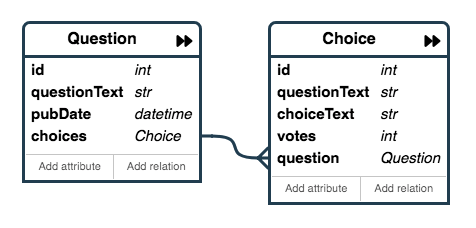
\includegraphics{images/django-entry.png}
\caption{模型数据关系图}
\end{figure}

在应用的\texttt{model.py}中写入如下代码:

\begin{Shaded}
\begin{Highlighting}[]
\ImportTok{from}\NormalTok{ django.db }\ImportTok{import}\NormalTok{ models}

\KeywordTok{class}\NormalTok{ Question(models.Model):}
\NormalTok{    question_text }\OperatorTok{=}\NormalTok{ models.CharField(max_length}\OperatorTok{=}\DecValTok{200}\NormalTok{)}
\NormalTok{    pub_date }\OperatorTok{=}\NormalTok{ models.DateTimeField(}\StringTok{'date published'}\NormalTok{)}

\KeywordTok{class}\NormalTok{ Choice(models.Model):}
\NormalTok{    question }\OperatorTok{=}\NormalTok{ models.ForeignKey(Question, on_delete}\OperatorTok{=}\NormalTok{models.CASCADE)}
\NormalTok{    choice_text }\OperatorTok{=}\NormalTok{ models.CharField(max_length}\OperatorTok{=}\DecValTok{200}\NormalTok{)}
\NormalTok{    votes }\OperatorTok{=}\NormalTok{ models.IntegerField(default}\OperatorTok{=}\DecValTok{0}\NormalTok{)}
\end{Highlighting}
\end{Shaded}

上述代码的作用,就是设置数据库中表的字段信息(字段名称、字段类型、字段属性等等)。

\hypertarget{ux6fc0ux6d3bux6a21ux578b}{%
\subsection{激活模型}\label{ux6fc0ux6d3bux6a21ux578b}}

有了字段信息,可以使用Django提供的指令,生成数据模型。

\begin{Shaded}
\begin{Highlighting}[]
\ExtensionTok{python}\NormalTok{ manage.py makemigrations polls}
\end{Highlighting}
\end{Shaded}

你将会看到类似于下面这样的输出:

\begin{Shaded}
\begin{Highlighting}[]
\ExtensionTok{Migrations}\NormalTok{ for }\StringTok{'polls'}\NormalTok{:}
  \ExtensionTok{polls/migrations}\NormalTok{/0001_initial.py:}
    \ExtensionTok{-}\NormalTok{ Create model Choice}
    \ExtensionTok{-}\NormalTok{ Create model Question}
\end{Highlighting}
\end{Shaded}

通过运行 \texttt{makemigrations} 命令,Django 会检测你对模型文件的修改(在这种情况下,你已经取得了新的),并且把修改的部分储存为一次\textbf{迁移}。所谓迁移,就是数据库结构变化的储存形式。

但是我们发现内置服务器输出一些警告信息:

\begin{Shaded}
\begin{Highlighting}[]
\ExtensionTok{You}\NormalTok{ have 17 unapplied migration(s)}\BuiltInTok{.} \ExtensionTok{Your}\NormalTok{ project may not work properly until you apply the migrations for app(s)}\BuiltInTok{:}\NormalTok{ admin, auth, contenttypes, sessions.}
\ExtensionTok{Run} \StringTok{'python manage.py migrate'}\NormalTok{ to apply them.}
\end{Highlighting}
\end{Shaded}

以上信息的意思是项目有一些迁移,但这些迁移没有执行,可能对运行产生影响。要执行迁移,就需要使用\texttt{migrate}指令:

\begin{Shaded}
\begin{Highlighting}[]
\ExtensionTok{python}\NormalTok{ manage.py migrate}
\end{Highlighting}
\end{Shaded}

在终端可以看到输出如下信息:

\begin{Shaded}
\begin{Highlighting}[]
\ExtensionTok{python}\NormalTok{ manage.py migrate}
\ExtensionTok{Operations}\NormalTok{ to perform:}
  \ExtensionTok{Apply}\NormalTok{ all migrations: admin, auth, contenttypes, sessions}
\ExtensionTok{Running}\NormalTok{ migrations:}
  \ExtensionTok{Applying}\NormalTok{ contenttypes.0001_initial... OK}
  \ExtensionTok{Applying}\NormalTok{ auth.0001_initial... OK}
  \ExtensionTok{Applying}\NormalTok{ admin.0001_initial... OK}
  \ExtensionTok{Applying}\NormalTok{ admin.0002_logentry_remove_auto_add... OK}
  \ExtensionTok{Applying}\NormalTok{ admin.0003_logentry_add_action_flag_choices... OK}
  \ExtensionTok{Applying}\NormalTok{ contenttypes.0002_remove_content_type_name... OK}
  \ExtensionTok{Applying}\NormalTok{ auth.0002_alter_permission_name_max_length... OK}
  \ExtensionTok{Applying}\NormalTok{ auth.0003_alter_user_email_max_length... OK}
  \ExtensionTok{Applying}\NormalTok{ auth.0004_alter_user_username_opts... OK}
  \ExtensionTok{Applying}\NormalTok{ auth.0005_alter_user_last_login_null... OK}
  \ExtensionTok{Applying}\NormalTok{ auth.0006_require_contenttypes_0002... OK}
  \ExtensionTok{Applying}\NormalTok{ auth.0007_alter_validators_add_error_messages... OK}
  \ExtensionTok{Applying}\NormalTok{ auth.0008_alter_user_username_max_length... OK}
  \ExtensionTok{Applying}\NormalTok{ auth.0009_alter_user_last_name_max_length... OK}
  \ExtensionTok{Applying}\NormalTok{ auth.0010_alter_group_name_max_length... OK}
  \ExtensionTok{Applying}\NormalTok{ auth.0011_update_proxy_permissions... OK}
  \ExtensionTok{Applying}\NormalTok{ sessions.0001_initial... OK}
\end{Highlighting}
\end{Shaded}

现在再启动内置服务器,之前的相关警告信息消失了。

\hypertarget{ux6570ux636eux5e93ux7684ux751fux6210ux4e0eux8fc1ux79fb}{%
\subsection{数据库的生成与迁移}\label{ux6570ux636eux5e93ux7684ux751fux6210ux4e0eux8fc1ux79fb}}

迁移是非常强大的功能,它能让你在开发过程中持续的改变数据库结构而不需要重新删除和创建表,迁移使得开发人员专注于使数据库平滑升级而不会丢失数据。改变模型需要这三步:

\begin{enumerate}
\def\labelenumi{\arabic{enumi}.}
\tightlist
\item
  编辑 \texttt{models.py} 文件,改变模型。
\item
  运行 \texttt{python\ manage.py\ makemigrations} 为模型的改变生成迁移文件。
\item
  运行 \texttt{python\ manage.py\ migrate} 来应用数据库迁移。
\end{enumerate}

数据库迁移被分解成生成和应用两个命令是为了让你能够在代码控制系统上提交迁移数据并使其能在多个应用里使用;这不仅仅会让开发更加简单,也给别的开发者和生产环境中的使用带来方便。

\hypertarget{ux540eux53f0ux7ba1ux7406}{%
\section{后台管理}\label{ux540eux53f0ux7ba1ux7406}}

Django 全自动地根据模型创建后台界面。管理界面不是为了网站的访问者,而是为管理者准备的。

\hypertarget{ux521bux5efaux7ba1ux7406ux5458ux8d26ux53f7}{%
\subsection{创建管理员账号}\label{ux521bux5efaux7ba1ux7406ux5458ux8d26ux53f7}}

Django 提供了功能全面的后台管理程序,首先我们增加超级管理员:

\begin{Shaded}
\begin{Highlighting}[]
\ExtensionTok{python}\NormalTok{ manage.py createsuperuser}
\end{Highlighting}
\end{Shaded}

输入用户名、邮箱、密码等信息后,Django会自动生成管理员账户信息。

\hypertarget{ux6dfbux52a0ux5f15ux7528ux5230ux540eux53f0ux7ba1ux7406}{%
\subsection{添加引用到后台管理}\label{ux6dfbux52a0ux5f15ux7528ux5230ux540eux53f0ux7ba1ux7406}}

打开 \texttt{polls/admin.py} 文件,在其中添加需要在后台管理的应用:

\begin{Shaded}
\begin{Highlighting}[]
\ImportTok{from}\NormalTok{ django.contrib }\ImportTok{import}\NormalTok{ admin}

\ImportTok{from}\NormalTok{ .models }\ImportTok{import}\NormalTok{ Question}

\NormalTok{admin.site.register(Question)}
\end{Highlighting}
\end{Shaded}

\hypertarget{ux8fdbux5165ux540eux53f0ux7ba1ux7406ux754cux9762}{%
\subsection{进入后台管理界面}\label{ux8fdbux5165ux540eux53f0ux7ba1ux7406ux754cux9762}}

\begin{Shaded}
\begin{Highlighting}[]
\ExtensionTok{python}\NormalTok{ manage.py runserve}
\end{Highlighting}
\end{Shaded}

在浏览器中\texttt{http://127.0.0.1:8000/admin/} 。你应该会看见管理员登录界面,输入之前设置的管理员信息后,就可以在后台管理界面中对数据进行操作。

\hypertarget{ux521bux5efaux89c6ux56fe-1}{%
\section{创建视图}\label{ux521bux5efaux89c6ux56fe-1}}

Django 中的视图的概念是「一类具有相同功能和模板的网页的集合」。在 Django 中,网页和其他内容都是从视图派生而来。每一个视图表现为一个简单的 Python 函数(或者说方法,如果是在基于类的视图里的话)。Django 将会根据用户请求的 URL 来选择使用哪个视图(更准确的说,是根据 URL 中域名之后的部分)。

为了将 URL 和视图关联起来,Django 使用了 `URLconfs' 来配置。URLconf 将 URL 模式映射到视图。

\hypertarget{ux6dfbux52a0ux591aux4e2aux89c6ux56fe}{%
\subsection{添加多个视图}\label{ux6dfbux52a0ux591aux4e2aux89c6ux56fe}}

现在再创建几个显示投票信息的页面,在 polls/views.py 中添加如下代码:

\begin{Shaded}
\begin{Highlighting}[]
\ImportTok{from}\NormalTok{ django.shortcuts }\ImportTok{import}\NormalTok{ render}
\ImportTok{from}\NormalTok{ django.http }\ImportTok{import}\NormalTok{ HttpResponse}

\KeywordTok{def}\NormalTok{ index(request):}
    \ControlFlowTok{return}\NormalTok{ HttpResponse(}\StringTok{"这是我的第一个视图。"}\NormalTok{)}

\KeywordTok{def}\NormalTok{ detail(request, question_id):}
    \ControlFlowTok{return}\NormalTok{ HttpResponse(}\StringTok{"你正在查看第 }\SpecialCharTok\NormalTok{ question_id)}

\KeywordTok{def}\NormalTok{ results(request, question_id):}
\NormalTok{    response }\OperatorTok{=} \StringTok{"你正在查看第 }\SpecialCharTok\NormalTok{ question_id)}

\KeywordTok{def}\NormalTok{ vote(request, question_id):}
    \ControlFlowTok{return}\NormalTok{ HttpResponse(}\StringTok{"你正在填写第 }\SpecialCharTok\NormalTok{ question_id)}
\end{Highlighting}
\end{Shaded}

每个视图必须要做的只有两件事:返回一个包含被请求页面内容的 HttpResponse 对象,或者抛出一个异常,比如 Http404 。至于你还想干些什么,随便你。

\hypertarget{ux6dfbux52a0ux8defux7531ux4fe1ux606f}{%
\subsubsection{添加路由信息}\label{ux6dfbux52a0ux8defux7531ux4fe1ux606f}}

为了显示上述视图,需要添加路由信息,方可访问。在 polls.urls 模块中,添加如下代码:

\begin{Shaded}
\begin{Highlighting}[]
\ImportTok{from}\NormalTok{ django.urls }\ImportTok{import}\NormalTok{ path}

\ImportTok{from}\NormalTok{ . }\ImportTok{import}\NormalTok{ views}

\NormalTok{urlpatterns }\OperatorTok{=}\NormalTok{ [}
\NormalTok{    path(}\StringTok{''}\NormalTok{, views.index, name}\OperatorTok{=}\StringTok{'index'}\NormalTok{),}
\NormalTok{    path(}\StringTok{'<int:question_id>/'}\NormalTok{, views.detail, name}\OperatorTok{=}\StringTok{'detail'}\NormalTok{),}
\NormalTok{    path(}\StringTok{'<int:question_id>/results/'}\NormalTok{, views.results, name}\OperatorTok{=}\StringTok{'results'}\NormalTok{),}
\NormalTok{    path(}\StringTok{'<int:question_id>/vote/'}\NormalTok{, views.vote, name}\OperatorTok{=}\StringTok{'vote'}\NormalTok{),}
\NormalTok{]}
\end{Highlighting}
\end{Shaded}

当某人请求你网站的某一页面时------比如说, ``/polls/34/'' ,Django 将会载入 mysite.urls 模块,因为这在配置项 ROOT\_URLCONF 中设置了。然后 Django 寻找名为 urlpatterns 变量并且按序匹配正则表达式。在找到匹配项 `polls/',它切掉了匹配的文本(``polls/''),将剩余文本------``34/'',发送至 `polls.urls' URLconf 做进一步处理。在这里剩余文本匹配了 `/',使得我们 Django 以如下形式调用 detail():

\begin{Shaded}
\begin{Highlighting}[]
\NormalTok{detail(request}\OperatorTok{=<}\NormalTok{HttpRequest }\BuiltInTok{object}\OperatorTok{>}\NormalTok{, question_id}\OperatorTok{=}\DecValTok{34}\NormalTok{)}
\end{Highlighting}
\end{Shaded}

\hypertarget{ux6a21ux7248ux547dux540dux7a7aux95f4}{%
\subsection{模版命名空间}\label{ux6a21ux7248ux547dux540dux7a7aux95f4}}

为什么要用模板?如果把页面的设计写死在视图函数的代码里,当想改变页面的样式是,就需要编辑 Python 代码。可使用 Django 的模板系统,只要创建一个视图,就可以将页面的设计从代码中分离出来。这样在逻辑上更加清晰,有利于项目的维护。

首先,在 polls 目录里创建一个 templates 目录。Django 将会在这个目录里查找模板文件。在你刚刚创建的 templates 目录里,再创建一个目录 polls,然后在其中新建一个文件 index.html 。换句话说,你的模板文件的路径应该是 polls/templates/polls/index.html 。因为 Django 会寻找到对应的 app\_directories ,所以你只需要使用 polls/index.html 就可以引用到这一模板了。

虽然我们现在可以将模板文件直接放在 polls/templates 文件夹中(而不是再建立一个 polls 子文件夹),但是这样做不太好。Django 将会选择第一个匹配的模板文件,如果你有一个模板文件正好和\textbf{另一个应用中的某个模板文件重名},Django 没有办法区分它们。我们需要帮助 Django 选择正确的模板,最简单的方法就是把他们放入各自的\textbf{命名空间}中,也就是把这些模板放入一个\textbf{和自身应用重名的子文件夹}里。

例如,\texttt{polls}的首页模板内容为:

\begin{Shaded}
\begin{Highlighting}[]
\NormalTok{\{}\OperatorTok\NormalTok{\}}
\OperatorTok{<}\NormalTok{ul}\OperatorTok{>}
\NormalTok{    \{}\OperatorTok\NormalTok{\}}
    \OperatorTok{<}\NormalTok{li}\OperatorTok{><}\NormalTok{a href}\OperatorTok{=}\StringTok{"\{}\SpecialCharTok{% u}\StringTok{rl 'polls:detail' question.id %\}"}\OperatorTok{>}\NormalTok{\{\{ question.question_text \}\}}\OperatorTok{</}\NormalTok{a}\OperatorTok{></}\NormalTok{li}\OperatorTok{>}
\NormalTok{    \{}\OperatorTok\NormalTok{\}}
\OperatorTok{</}\NormalTok{ul}\OperatorTok{>}
\NormalTok{\{}\OperatorTok\NormalTok{\}}
\OperatorTok{<}\NormalTok{p}\OperatorTok{>}\NormalTok{No polls are available.}\OperatorTok{</}\NormalTok{p}\OperatorTok{>}
\NormalTok{\{}\OperatorTok\NormalTok{\}}
\end{Highlighting}
\end{Shaded}

\hypertarget{ux5728ux89c6ux56feux4e2dux4f7fux7528ux6a21ux677f}{%
\subsection{在视图中使用模板}\label{ux5728ux89c6ux56feux4e2dux4f7fux7528ux6a21ux677f}}

在视图\texttt{polls/view.py}中,载入模板、填充上下文,再返回由它生成的\texttt{HTTPResponse}对象,这就是在视图中使用模板的常用流程,Django 为此提供了一个快捷函数:\texttt{render()}

\begin{Shaded}
\begin{Highlighting}[]
\ImportTok{from}\NormalTok{ django.http }\ImportTok{import}\NormalTok{ HttpResponse}
\ImportTok{from}\NormalTok{ .models }\ImportTok{import}\NormalTok{ Question}

\KeywordTok{def}\NormalTok{ index(request):}
\NormalTok{    latest_question_list }\OperatorTok{=}\NormalTok{ Question.objects.order_by(}\StringTok{'-pub_date'}\NormalTok{)[:}\DecValTok{5}\NormalTok{]}
\NormalTok{    context }\OperatorTok{=}\NormalTok{ \{}
        \StringTok{'latest_question_list'}\NormalTok{: latest_question_list,}
\NormalTok{    \}}
    \ControlFlowTok{return}\NormalTok{ render(request,}\StringTok{'polls/index.html'}\NormalTok{,context)}
\end{Highlighting}
\end{Shaded}

\hypertarget{urlux547dux540dux7a7aux95f4}{%
\subsection{URL命名空间}\label{urlux547dux540dux7a7aux95f4}}

在一个真实的 Django 项目中,可能会有五个,十个,二十个,甚至更多应用。Django 如何分辨重名的 URL 呢?举个例子,polls 应用有 detail 视图,可能另一个博客应用也有同名的视图。Django 如何知道 \texttt{\{\%\ url\ \%\}} 标签到底对应哪一个应用的 URL 呢?

答案是:在根 URLconf 中添加命名空间。在 \texttt{polls/urls.py} 文件中稍作修改,加上 \texttt{app\_name} 设置命名空间:

\begin{Shaded}
\begin{Highlighting}[]
\NormalTok{app_name }\OperatorTok{=} \StringTok{'polls'}
\end{Highlighting}
\end{Shaded}

对应的,在模板文件中,将原来的URL编码:

\begin{Shaded}
\begin{Highlighting}[]
\OperatorTok{<}\NormalTok{li}\OperatorTok{><}\NormalTok{a href}\OperatorTok{=}\StringTok{"/polls/}\SpecialCharTok{\{\{}\StringTok{ question.id }\SpecialCharTok{\}\}}\StringTok{/"}\OperatorTok{>}\NormalTok{\{\{ question.question_text \}\}}\OperatorTok{</}\NormalTok{a}\OperatorTok{></}\NormalTok{li}\OperatorTok{>}
\end{Highlighting}
\end{Shaded}

修改为:

\begin{Shaded}
\begin{Highlighting}[]
\OperatorTok{<}\NormalTok{li}\OperatorTok{><}\NormalTok{a href}\OperatorTok{=}\StringTok{"\{}\SpecialCharTok{% u}\StringTok{rl 'polls:detail' question.id %\}"}\OperatorTok{>}\NormalTok{\{\{ question.question_text \}\}}\OperatorTok{</}\NormalTok{a}\OperatorTok{></}\NormalTok{li}\OperatorTok{>}
\end{Highlighting}
\end{Shaded}

这样做的好处是,当你想改变投票详情视图的 URL,比如想改成 \texttt{polls/specifics/12/} ,你不用在模板里修改任何东西(包括其它模板),只要在 \texttt{polls/urls.py} 里稍微修改即可,实现了模板和路由的部分解耦。

\hypertarget{ux6a21ux578b}{%
\section{模型}\label{ux6a21ux578b}}

在 Django 中,\textbf{模型}在形式上是定义数据表的文件,并没有提供数据查询之类的功能,这一点,是 Django 框架非常不同与其他框架的地方,Django 将数据查询检索的功能安排在\textbf{视图}中。模型包含您数据的重要字段和行为。一般来说,每一个模型都映射一个数据库表。每个模型都是一个 Python 的类,这些类继承 \texttt{django.db.models.Model},模型类的每个属性都相当于一个数据库的字段。Django 会根据字段信息,生成数据库以及访问数据库的 API。

\hypertarget{ux8bbeux7f6eux6570ux636eux5e93ux4fe1ux606f-1}{%
\subsection{设置数据库信息}\label{ux8bbeux7f6eux6570ux636eux5e93ux4fe1ux606f-1}}

Django 默认使用 SQLite 数据库,该数据库性能有限。通常我们使用 MySQL/MariaDB 或者 MongoDB 之类的数据库。下面以 MySQL 为例,设置 Django 数据库信息。

\begin{enumerate}
\def\labelenumi{\arabic{enumi}.}
\item
  安装 MySQL,并设置好数据库信息,注意数据库编码方式设置为\texttt{utf8mb4}。
\item
  使用 pip 安装 pymysql 库
\item
  在 Django 中的项目文件\texttt{settings.py}中添加如下配置信息:

\begin{Shaded}
\begin{Highlighting}[]
\ImportTok{import}\NormalTok{ pymysql}
\NormalTok{pymysql.install_as_MySQLdb()}
\NormalTok{DATABASES }\OperatorTok{=}\NormalTok{ \{}
     \StringTok{'default'}\NormalTok{: \{}
         \StringTok{'ENGINE'}\NormalTok{: }\StringTok{'django.db.backends.mysql'}\NormalTok{,}
         \StringTok{'NAME'}\NormalTok{: }\StringTok{'xxx'}\NormalTok{,  }\CommentTok{# 数据库名,可以自己创建用户}
         \StringTok{'USER'}\NormalTok{: }\StringTok{'xxx'}\NormalTok{,  }\CommentTok{# 用户名,可以自己创建用户}
         \StringTok{'PASSWORD'}\NormalTok{: }\StringTok{'xxx'}\NormalTok{,  }\CommentTok{# 密码}
         \StringTok{'HOST'}\NormalTok{: }\StringTok{'192.168.1.108'}\NormalTok{,  }\CommentTok{# mysql服务所在的主机ip}
         \StringTok{'PORT'}\NormalTok{: }\StringTok{'3306'}\NormalTok{,}
\NormalTok{     \}}
\NormalTok{ \}}
\end{Highlighting}
\end{Shaded}
\end{enumerate}

\hypertarget{ux521bux5efaux6a21ux578b-1}{%
\subsection{创建模型}\label{ux521bux5efaux6a21ux578b-1}}

模型需要继承自\texttt{django.db.models.Model}。例如:

\begin{Shaded}
\begin{Highlighting}[]
\ImportTok{from}\NormalTok{ django.db }\ImportTok{import}\NormalTok{ models}

\KeywordTok{class}\NormalTok{ Person(models.Model):}
\NormalTok{    first_name }\OperatorTok{=}\NormalTok{ models.CharField(max_length}\OperatorTok{=}\DecValTok{30}\NormalTok{)}
\NormalTok{    last_name }\OperatorTok{=}\NormalTok{ models.CharField(max_length}\OperatorTok{=}\DecValTok{30}\NormalTok{)}
\end{Highlighting}
\end{Shaded}

\hypertarget{ux5b57ux6bb5ux7c7bux578b}{%
\subsubsection{字段类型}\label{ux5b57ux6bb5ux7c7bux578b}}

Django 框架能根据模型中的字段信息自动生成如下几类信息:

\begin{enumerate}
\def\labelenumi{\arabic{enumi}.}
\tightlist
\item
  数据表中的字段
\item
  表单中对应的 HTML 元素
\item
  后台管理中的 HTML 页面及表单
\end{enumerate}

在创建模型和字段的时候,和其他变量、类、对象命名一样,不能使用 Python 的关键字、保留字以及 SQL 语句中的关键字,也不能使用和 Django 框架中有冲突的名字(不能在变量名中使用两个下划线,如\texttt{foo\_\_bar},变量命中使用两个下划线在 Django 中有查询等功能)。

常用的 Django 模型字段类型有:

\begin{longtable}[]{@{}ll@{}}
\toprule
类型 & 作用\tabularnewline
\midrule
\endhead
BooleanField & 布尔值字段\tabularnewline
CharField & 字符串字段\tabularnewline
DateField & 日期字段\tabularnewline
DateTimeField & 日期时间字段\tabularnewline
EmailField & 电子邮箱字段\tabularnewline
FileField & 文件上传字段\tabularnewline
\bottomrule
\end{longtable}

\hypertarget{ux4f7fux7528ux6a21ux578b}{%
\subsection{使用模型}\label{ux4f7fux7528ux6a21ux578b}}

\begin{enumerate}
\def\labelenumi{\arabic{enumi}.}
\item
  定义好模型后,需要修改设置文件中的 \texttt{INSTALLED\_APPS} ,在这个设置中添加包含你 \texttt{models.py} 文件的模块的名字。
\item
  在命令行中运行\texttt{python\ manage.py\ makemigrations},创建数据库迁移文件。
\item
  执行数据库迁移:

\begin{Shaded}
\begin{Highlighting}[]
\ExtensionTok{python}\NormalTok{ manage.py migrate}
\end{Highlighting}
\end{Shaded}
\item
  如有必要,将模型在后台页面中显示出来。
\end{enumerate}

\hypertarget{ux53c2ux8003ux6587ux732e-1}{%
\section{参考文献}\label{ux53c2ux8003ux6587ux732e-1}}

\begin{enumerate}
\def\labelenumi{\arabic{enumi}.}
\tightlist
\item
  \href{https://docs.djangoproject.com/zh-hans/2.2/intro/tutorial01/}{编写你的第一个 Djongo 应用}
\item
  \href{https://docs.djangoproject.com/zh-hans/2.2/intro/tutorial02/}{数据库配置及模型创建}
\item
  \url{https://docs.djangoproject.com/zh-hans/2.2/intro/tutorial03/}
\end{enumerate}

\bibliography{book.bib,packages.bib}

\backmatter
\printindex

\end{document}
